% GUIDA VELOCE:
% --------------------------------------------------------------------
% X INIZIA UN UNOVO CAPITOLO:
% \chapter{??? NOME CAPITOLO}}
% \section{ ?? }
% \subsection{ ?? }
%
% --------------------------------------------------------------------
% PAROLA CONTENUTA NEL GLOSSARIO:
% scrivere la parola seguita da $^g$
% esempio: User$^g$
%
% --------------------------------------------------------------------
% PER ANDARE A CAPO SENZA RIENTRO INSERIRE:
% \\
%
% --------------------------------------------------------------------

% GRASSETO:
% \textbf{parola}
%
% --------------------------------------------------------------------
% CORSIVO:
% \emph{parola}
% --------------------------------------------------------------------
% PER SCRIVERE IN ROSSO:
% \red{parola}
%
% --------------------------------------------------------------------
% PER SCRIVERE TRA VIRGOLETTE
% ''parola''
%
% --------------------------------------------------------------------
% PER EVITARE IL RIENTRO AUTOMATICO DI UN CAPOVERSO:
% \noindent testo....
%
% --------------------------------------------------------------------

% PER SCRIVERE CARATTERI PARTICOLARI COME: { } _ ecc.. SCRIVERLI PRECEDUTI DA \
% ES: \{ \_
%
% --------------------------------------------------------------------
% X INSERIRE UN LINK:
% \url{http://www.math.unipd.it/~tullio/IS-1/2011/Progetto/C3.pdf}
%
% --------------------------------------------------------------------
% PER COMMENTARE INTERE PARTI:
% \comment{ comment }
%
% --------------------------------------------------------------------
% PER SCRIVERE NOTE DURANTE IL TESTO:
% parola \footnote{ note riguardanti la parola }
%
% --------------------------------------------------------------------
% PER SCRIVERE CODICE SORGENTE:
%
% \lstset{language=c++,
% stringstyle=\color{blue}\textrm,
% commentstyle=\rmfamily, numbers= none}

% \begin{lstlisting}
% CODICE
% \end{lstlisting}
%
% --------------------------------------------------------------------
% !!!!!!!! PER COSE + COMPLESSE VEDI: !!!!!!!!!!!!!!!!!!!!!!!
% !!!!!!!! PMAC/latex/GUIDA LATEX!!!.tex !!!!!!!!!!!!!!!!!!!!!!!

% per tutto il resto chiedi a lory prima di fare/scrivere cazzate !!!!!!!!!!



\documentclass[10pt,a4paper]{book}

\usepackage[italian]{babel}
\usepackage[T1]{fontenc}
\usepackage[utf8x]{inputenc} % uso utf8x xk x linux, mentre latin1 è per windows
\usepackage{lmodern} %insieme di font molto completo consigliato da LatexFacile pg13 in basso
\usepackage{microtype} %migliora riempimento delle righe. vedi LatexImpaziente pg41
%attiva il rientro di ogni prima riga di ogni sezione: capitolo,paragrafo ecc. vd LatexImpaziente pg41
\usepackage{indentfirst}
\usepackage{graphicx} % per inseire immagini
\usepackage[usenames,dvipsnames]{color}
\usepackage{lastpage} %serve per poter scrivere page 1 of N
% setta i bordi della pagina: dx e sx 3.2cm di rientro + nel lato di rilagatura rientra di altri 0mm
\usepackage[a4paper,top=3cm,bottom=3cm,left=3.2cm,right=3.2cm, bindingoffset=0mm]{geometry}
\usepackage{listings} % per inserire codice sorgente
\usepackage{float} % per gestire oggetti flottanti ( es immagini tabelle posizionebili con "H" che forza il posizionamento nel punto specifico )
\usepackage{marvosym} % per \EUR
\usepackage[Bjornstrup]{fncychap} % serve per customizzare i capitoli con il book

% serve per creare tabelle lunghe + di una pagina con \begin{longtable} (vd Tabelle.pdf pg11-12)
\usepackage{longtable}

\usepackage{fancyhdr} % per impostare lo stile della pagina più personalizzato, + fancyhdr ( per regolare testatina e piè di pagina ) vedi itfancyhrd


\pagestyle{fancy}
% settaggi di pagestyle(fancy)
\lhead{
\includegraphics[scale=0.20]{images/SevenFold_small}}
%\chead{}
\rhead{\textbf{{%
\NomeDocumento \\ Data: \DataRilascio \\ e-mail: \mail{sevenfold@palomino.it}}}}
\lfoot{\NomeDocumento}
\cfoot{}
\rfoot{ \textbf \thepage\ di \pageref{LastPage}}
\renewcommand{\footrulewidth}{0.4pt}

%ridefinisco il plain per cosare l'indice (a questo punto si potrebbe lasciare tutto il documento in plain
\fancypagestyle{plain}{
\lhead{
\includegraphics[scale=0.20]{images/SevenFold_small}}
%\chead{}
\rhead{\textbf{{%
\NomeDocumento \\ Data: \DataRilascio \\ e-mail: \mail{sevenfold@palomino.it}}}}
\lfoot{\NomeDocumento}
\cfoot{}
\rfoot{ \textbf \thepage\ di \pageref{LastPage}}
\renewcommand{\footrulewidth}{0.4pt}
}

% da ultimo:
\usepackage{hyperref} %x l'interpretazione di indirizzi o link ipertestuali (vd LatexImpaziente pg47 )
\hypersetup{backref, colorlinks=true, linkcolor=black, urlcolor=black}

\usepackage{url} % x l'interpretazioni di internet o link ipertestuali (vd LatexImpaziente pg47 )
%\UrlFont{color =blue}
%\urlstyle{helvetic}

% Define a new 'leo' style for the package that will use a smaller font.
\makeatletter
\def\url@leostyle{%
  \@ifundefined{selectfont}{\def\UrlFont{\sf}}{\def\UrlFont{\small\ttfamily}}}
\makeatother
%% Now actually use the newly defined style.
\urlstyle{leo}


\newcommand{\mail}[1]{\textcolor{Black}{ \texttt{#1}}} %per interpretare mail (vd LatexImpaziente pg47 )
\newcommand{\cambiaFont}[2]{{\fontencoding{T1}\fontfamily{#1}\selectfont#2}}
\newcommand{\red}[1]{ \textcolor{red}{#1} } % per scrivere testo in rosso
\newcommand{\comment}[1]{} % per inserire commenti

\newcommand{\attribute}[2]{ \item[\textcolor{PineGreen}{ \texttt{#1}}] \textcolor{PineGreen}{\texttt{#2\\}}\ \ \ }
\newcommand{\method}[2]{ \item[\textcolor{MidnightBlue}{ \texttt{#1}}] \textcolor{MidnightBlue}{ \texttt{#2\\}}\ \ \ }

\newcommand{ \class}[1]{ \item[-] \texttt{#1} }
\newcommand{\virgolette}[1]{``{#1}''}



% INSERIRE QUI IL NOME DEL DOCUMENTO SEGUITO DA UNO SPAZIO
% ( così il nome si imposta in automatico nelle varie ricorrenze standard)
\newcommand{\NomeDocumento}{Woty - Analisi di progetto}

% INSERIRE QUI LA DATA DEL RILASCIO DELLA VERSIONE ATTUALE
\newcommand{\DataRilascio}{2012/09/19}

% INSERIRE LA VERSIONE ATTUALE
%\newcommand{\VersioneAttuale}{v2.0.0}

% INSERIRE QUI L'ACRONIMO DEL DOCUMENTO. ESEMPIO: Analisi Dei Requisiti = AR
% Quando inserite l'acronimo qui, dovete rinominare i file presenti nella cartella
% del tipo '??-cap1-NomeCapitolo.tex' sostituendo i '??' con l'acronimo scelto!!
\newcommand{\AcronimoDocumento}{DP}

\begin{document}


% --------------------------------------------------------------------

% TITOLO ( 1° pagina)

\vspace*{2.5cm}
\begin{center}

%\cambiaFont{Cyklop}{Sevenfold}
%\cambiaFont{fve}{\Huge{Sevenfold}}

\includegraphics[scale=0.35]{images/SevenFold_big}

\vspace{2cm}

\cambiaFont{fve}{\Huge{\NomeDocumento}}\\
\vspace*{1cm}


\end{center}


% --------------------------------------------------------------------

% INFORMAZIONI DEL DOCUMENTO ( 1° pagina)

\vspace*{2cm}
\begin{center}

\begin{tabular}{ r | l }
\multicolumn{2}{c}{\textbf{\huge{Informazioni sul documento}} }\\
\hline
\rule[-1.5mm]{0mm}{0.7cm}
\textbf{Titolo documento} & \NomeDocumento\\
\rule[-1.5mm]{0mm}{0.5cm}
\textbf{Data creazione}& 2012/02/15\\
\rule[-1.5mm]{0mm}{0.5cm}
\textbf{Distribuito da}& Gruppo SevenFold\\
\rule[-1.5mm]{0mm}{0.5cm}
\textbf{Destinato a}&Prof. Ghiraldo Filippo\\
&Gruppo Sevenfold\\

\end{tabular}

\end{center}

% --------------------------------------------------------------------

% SOMMARIO ( 2° pagina)

\newpage

\vspace*{0.5cm} % il vertical space va preceduto da una riga vuota!!!
\begin{center}

\textbf{{\huge{Sommario}}}

Questo documento contiene i risultati dell' analisi del possibile business model e la documentazione sulla gestione della piattaforma Woty, effettuati durante il corso di Sviluppo e Gestione di Progetti.

\vspace*{0.2cm} % il vertical space va preceduto da una riga vuota!!!

\end{center}


% --------------------------------------------------------------------



% --------------------------------------------------------------------
% INDICI:

\newpage

% INDICE CAPITOLI
\tableofcontents % genera l'indice di tutto il documento

\let\cleardoublepage\clearpage % toglie la pagina bianca dopo l'indice

% INDICE TABELLE
\listoftables

% INDICE FIGURE
\listoffigures


% --------------------------------------------------------------------


\newpage
%####################################################
%   cap Luca Guerrra
%####################################################
\chapter{Descrizione del Prodotto}

Di seguito  viene presentato il sistema Woty, descrivendo le funzionalità pratiche del sistema, dagli attori coinvolti ai vari ambiti di utilizzo, al fine di rendere chiaro a un soggetto esterno l'effettiva utilità del prodotto.



\section{Cos'è Woty}

Il sistema software Woty si pone come obiettivo la realizzazione di una piattaforma innovativa per l'apprendimento comportamentale nell'ambito della sicurezza del lavoro, che utilizzi le tecniche della gamification per incentivare il coinvolgimento e la partecipazione degli utenti e per scardinare l'instaurarsi di abitudini errate.\\
Woty è orientato alla \virgolette{quest}, che consiste in un compito/sfida che l'utente dovrà compiere.\\
Questo permetterà al sistema di assegnare un punteggio, che concorrerà alla creazione di classifiche personali o di gruppo.\\
Woty vuole poter essere utilizzato sia in ambito aziendale su postazioni fisse (indipendentemente dall'OS utilizzato), sia in ambito mobile, attraverso l'utilizzo di smartphone.

\section{Collocazione del prodotto}

Il sistema software Woty può essere adottato da qualsiasi realtà lavorativa dove l'uso del computer rientra nella normale routine dei dipendenti.\\
I clienti che decidono di usare Woty offrono ai loro impiegati la possibilità di sostituire un eventuale corso frontale sulla sicurezza con l'utilizzo del nostro sistema.\\
In ambito aziendale la formazione del personale riguardo conoscenze critiche, come può essere ad esempio la gestione delle norme sulla sicurezza sul lavoro, è normalmente erogata secondo procedure statiche scollegate dall'ambiente lavorativo come l'insegnamento in aula, che poco motivano e stimolano all'apprendimento i partecipanti.\\
Un apprendimento diverso, di forma continua e interattiva, può essere erogato ai lavoratori come parte integrante delle attività lavorative standard, per fare in modo che il coinvolgimento dell'utente sia elevato, grazie a compiti e sfide a cui verrà sottoposto.\\
Un aumento dell'interesse e della partecipazione del lavoratore può essere creato attraverso elementi di gamification, con i quali verrà innestata una forma di competizione tra le diverse squadre di lavoro, oltre che nel singolo.

\section{Funzionalità del prodotto}

Di seguito sono descritte in generale le funzionalità che il sistema fornisce ai suoi utenti.

\subsection{Ambiente aziendale}
Nell'ambiente aziendale, Woty permette agli User di portare a termine le quest direttamente all'interno di un browser. Un sistema di notifica nel terminale dello User lo informa della presenza di nuove quest disponibili. Il sistema di notifica gestirà anche l'autenticazione al sistema.\\ 
È prevista in ogni azienda la presenza di un Super-user per l'amministrazione delle utenze.


\subsection{Ambiente mobile}
Gli User in mobilità denominati Mobile-user, tramite l'applicazione dedicata, si autenticano, svolgono le quest loro assegnate e visualizzano statistiche e punteggi esattamente come farebbero con la normale interfaccia desktop.

\section{Ambiente di esecuzione}
Il software è sviluppato sul modello client-server. I client si dividono in desktop e mobile. La parte server è ospitata unicamente presso le macchine del fornitore.\\
L'inserimento di un nuovo cliente comporta un intervento sull'interfaccia web da parte del Woty Administrator, che fissa inoltre il numero di account istanziabili dal nuovo cliente.\\
Viene designato un Super-user presso il cliente che tramite un'interfaccia web avrà le responsabilità di:
\begin{itemize}
\item{ Assegnare i singoli account utente al personale. }
\item{ Associare ad ogni account un workgroup che ne identifica il dipartimento (e.g. impiegato, operaio, etc.) scelta da un pool di workgroup assegnato all'azienda dal Woty Administrator. }
\end{itemize}

A questo punto la normale amministrazione del sistema è in mano al Super-user, che non dovrebbe avere bisogno del fornitore a meno di guasti.

\subsection{Server}
Il software va installato, inizializzato e testato presso gli appositi server interni.\\
L'uso è ridotto alla gestione amministrativa tramite interfaccia web, che deve poter essere portata a termine anche da personale qualificato ma non necessariamente tecnico.

\newpage

\subsection{Client Desktop}
Dopo l'assegnazione di un account da parte del Super-user, il primo contatto dello User con il sistema è la visita alla homepage del software che aiuta, tramite un wizard, l'installazione del demone per la gestione dell'autenticazione e delle notifiche.\\
Come riportiamo nei dati a seguire, vista la larga diffusione e uso della rete internet nel nostro paese, si presuppone che un utente medio sia in grado di svolgere senza difficoltà tutte le operazioni richieste, quindi non dovrebbe essere necessario l'aiuto di personale specifico per i passi precedentemente descritti.\\
Da questo punto per l'utente può cominciare la partecipazione attiva.\\


\begin{figure}[H]
\centering
\caption{Statistiche utilizzo internet in Italia}
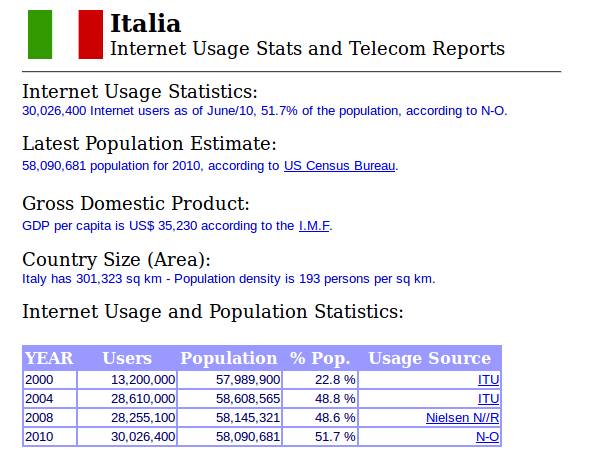
\includegraphics[scale=0.5]{images/cap1/statItaly} 
\end{figure}

\newpage
Inoltre, l'interfaccia web sarà sviluppata tale da rimanere inalterata se visualizzata con diversi browser, anche con differenti versioni.\\
Riportiamo di seguito le statistiche percentuali sull'utilizzo dei browser aggiornate a giugno 2012.

\begin{figure}[H]
\centering
\caption{Statistiche utilizzo browser}
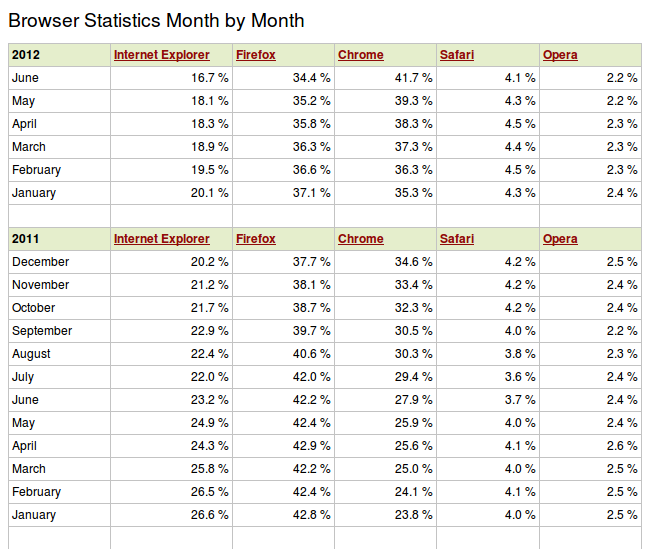
\includegraphics[scale=0.5]{images/cap1/internetStat} 
\end{figure}


\subsection{Client Mobile}
Per ogni dispositivo è disponibile un client distribuito a seconda della piattaforma in uso.\\
Dopo la canonica inizializzazione e assegnazione di un account da parte del Super-user, lo User può direttamente autenticarsi e cominciare a operare tramite l'interfaccia dell'applicazione.\\ 
Un Mobile-user ha inoltre la facoltà di agire esattamente come un Desktop-user tramite l'interfaccia web.\\
Dopo un'attenta valutazione e in base ai criteri di seguito esposti, abbiamo deciso di sviluppare inizialmente l'applicazione solo su dispositivi Android.\\
Nulla vieta, in futuro, di poter sviluppare l'applicazione anche per diversi sistemi.

\begin{figure}[H]
\centering
\caption{Statistiche d'uso dispositivi Android}
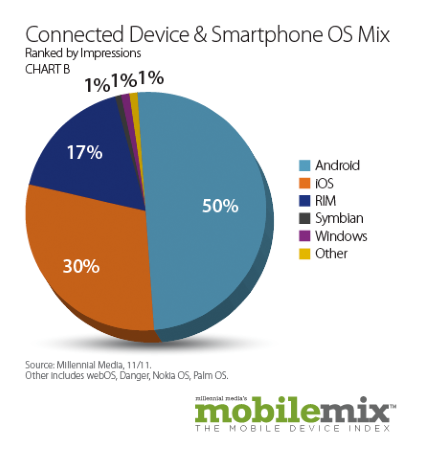
\includegraphics[scale=0.50]{images/cap1/statAndroid} 
\end{figure}

Per quanto riguarda la scelta della versione da utilizzare abbiamo seguite le seguenti statistiche; gli aspetti tecnici tuttavia verranno trattati più dettagliatamente nei prossimi capitoli.\\

\begin{figure}[H]
\centering
\caption{Statistiche ufficiali Api}
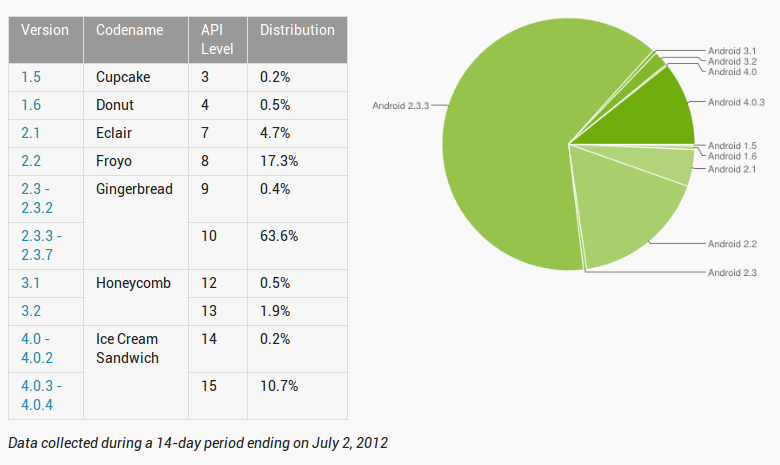
\includegraphics[scale=0.55]{images/cap1/api} 
\end{figure}

\newpage

\subsection{Caratteristiche degli utenti}
Gli attori chiamati in causa si suddivideranno nelle seguenti categorie:

\begin{enumerate}

\item \textbf{Woty Administrator}\\
L'attività assegnata al Woty Administrator è quella di illustrare il funzionamento del software.\\
E' incaricato dell'inserimento delle quest. Conoscenze pratiche richieste: gestione di sistemi e reti informatiche.

\item \textbf{Desktop-user}, a loro volta divisi in:

\begin{enumerate}

\item \textbf{Desktop-user} senza dispositivo mobile\\
Questo tipo di attore dovrà svolgere le varie quest assegnategli da postazione fissa;

\item \textbf{Desktop-user} con dispositivo mobile\\
Questo tipo di attore dovrà svolgere le varie quest assegnategli, inoltre potrà averne a disposizione altre specifiche in cui si richiede l'uso di un dispositivo mobile (e.g. rilevamento di QR-Code).

\end{enumerate}

\item \textbf{Mobile-user}\\
Questa tipologia di utenti potrà svolgere le proprie quest direttamente dal dispositivo mobile, quindi senza essere fisicamente nell'azienda.\\
Per entrambi gli attori Desktop-user e Mobile-user non sono richieste particolari conoscenze informatiche.

\item \textbf{Super-user}\\
Il Super-user sarà colui che all'interno dell'azienda dovrà occuparsi di visionare i risultati delle varie quest ed eventualmente illustrarne il funzionamento agli User. Si occupa inoltre dell'assegnazione di workgroup agli User del sistema.

\end{enumerate}

\newpage

\section{Descrizione quest}

Le tipologie di quest che un User può sostenere sono varie, caratterizzate da un input che Woty darà all'utente e da una risposta che l'utente darà al sistema, in base alle richieste.\\
SevenFold si riserva di ampliare e/o modificare le tipologie di quest offerte durante lo sviluppo di Woty.

\subsection{Caratterizzazione in base all'input Woty -> User}
\begin{itemize}
\item Testo: l'User visualizzerà un semplice testo.
\item Foto: l'User visualizzerà a video un'immagine.
\item Video: l'User visualizzerà un filmato.
\end{itemize}

\subsection{Caratterizzazione in base alla risposta dell'User}
\begin{itemize}
\item Risposta secca (si/no, vero/falso)
\item Risposta chiusa tra un certo numero alternative
\item Risposta multipla tra un certo numero di opzioni
\item In caso di quest basata su testi, possibilità di riordinare testi disordinati
\item In caso di quest basata su foto, possibilità di riordinare foto spezzettata e disordinata (puzzle)
\item Scansione di un QR-Code (Mobile-user)
\end{itemize}

\subsection{Caratterizzazione in base al tempo di risoluzione}
\begin{itemize}
\item Standard: quest senza un limite di tempo di risoluzione.
\item Temporizzata: quest con un limite di tempo di risoluzione.
\end{itemize}





% --------------------------------------------------------------------



%####################################################
%   cap Pretto
%####################################################
\chapter{Dettagli tecnici}


In questo capitolo viene descritta la parte tecnica del softaware e implementazioni progettistiche architetturali. 

\section{Woty - Scelte architetturali}
In questa sezione verranno discusse le principali scelte architetturali che hanno portato alla realizzazione di Woty. 

\subsection{Approccio Client - Server}

\begin{center}
\begin{figure}[ht]
\centering
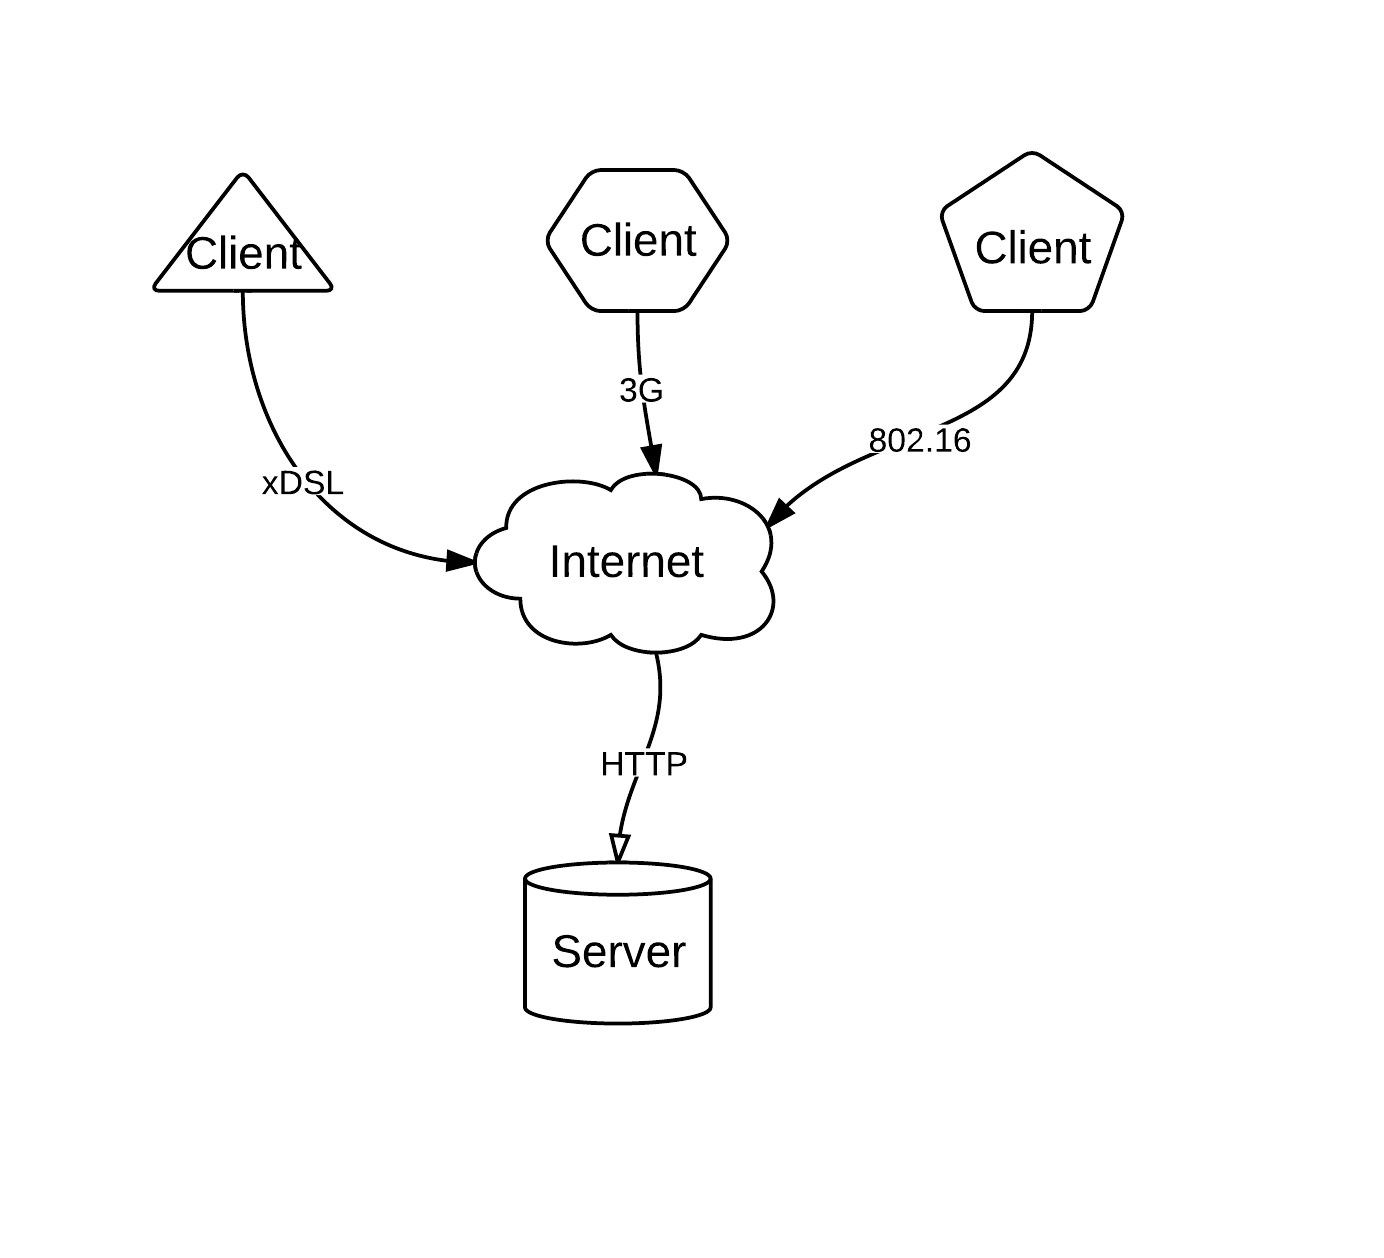
\includegraphics[scale=0.55]{images/cap2/Client-server.png}
\caption{Rappresentazione astratta architettura Client-Server}
\end{figure}
\end{center}

Il nucleo di Woty, dove viene gestita tutta la logica e vengono mantenuti i dati, risiede su un server centrale. Il server ospita il DBMS contenente i dati persistiti e l'applicazione web che tramite tali dati permette l'interazione con il sistema.\\
Woty è progettata per essere indipendente dal tipo di client che si interfaccerà con il server. Questo è garantito da un approccio orientato alla risorsa e da delle reference API standard. In questo modo la futura estensibilità di Woty verso nuovi tipi di client è non solo possibile, ma soprattutto semplice e realizzabile tramite un minimo costo implementativo.\\


\subsection{Woty: orientato alla risorsa}
Ogni ''elemento'' interno di woty (e.g. una quest, un utente, un achievement, etc) è offerto all'esterno come \emph{risorsa}. Questo permette la realizzazione di un approccio standard al webservice e garantisce massima estendibilità. \\
Ogni risorsa è disponibile all'esterno secondo precise regole di business (autorizzazioni, gestione della visibilità, etc.) in modo da aver sì un approccio standard, ma allo stesso tempo di avere un elevato grado di sicurezza, di incapsulamento delle informazioni e una personalizzazione ad-hoc per ogni risorsa senza limiti prestabiliti.


\subsection{Approccio RESTful}

Representational State Transfer, di seguito REST, è uno stile architetturale che permette la modellazione dei \emph{business models} tramite \emph{resources} (risorse). Le risorse sono rese accessibili tramite protocollo HTTP sotto forma di web services, e disponibili in varie \emph{representations}. Ogni risorsa espone metodi CRUD (\emph{create}, \emph{read}, \emph{update}, \emph{delete}) che vengono mappati su get, put, post, delete del protocollo HTTP. Il software che adotta questo tipo di struttura è definito come ''orientato alla risorsa''.\\

La tipologia di rappresentazione della risorsa richiesta è identificata sull'estensione del file identificato all'interno dell'uri. Ad esempio, una delle rappresentazioni disponibili è quella che incapsula le informazioni in sorgenti interpretabili da un web browser.\\ 

Un'altra caratteristica di questo approccio è la mancanza di necessità di tenere traccia dello stato. Ogni metodo è sempre disponibile o nascosto, senza dipendenze dallo stato del processo in esecuzione.\\ 
Tramite questa architettura si ottengono:

\begin{itemize}
			
\item Possibilità di comporre semplici richieste relazionali direttamente da uri.

\item API pubblica e autenticata, senza necessità di duplicazione di codice

\item Interfaccia di comunicazione tra i gli strati presentation e logic

\item Stretto legame con le risorse effettivamente presenti su database

\item State-less design (anche le sessioni sono modellate su risorse)

\item Sicurezza concentrata su singolo componente (HTTPS)
			
\item Disaccoppiamento tra i due strati comunicanti
\end{itemize}

Questo tipo di approccio aumenta l'estensibilità e la scalabilità del software. Rende inoltre il codice uniformato per risorse, facilmente comprensibile quindi meno dipendente dalle competenze del programmatore. \\
L'effettiva implementazione del webservice mappa tramite uri non solamente i metodi CRUD ma anche le operazioni (azioni index, show, edit) utili alla effettiva esecuzione dei metodi.\\
I seguenti metodi sono esplicitati maggiormente nel paragrafo \ref{resource}.
		
\begin{longtable}{|p{3cm}|p{5,0cm}|p{3cm}|}
\caption{HTTP/URI/CRUD}\\
\hline
\endfirsthead
\multicolumn{3}{r}{\textit{(Continua alla pagina successiva)}}
\endfoot
\multicolumn{3}{l}{\textit{(Continua dalla pagina precedente)}}
\endhead
\hline
\endlastfoot
\textbf{HTTP Verb} & \textbf{URI}& \textbf{Action}\\
\hline
POST & /resource & CREATE (C)\\
\hline
GET & /resource/id & SHOW (R)\\
\hline
PUT & /resource/id & UPDATE (U)\\
\hline
DELETE & /resource/id & DELETE (D)\\
\hline
GET & /resource & INDEX\\
\hline
GET & /resource/new & NEW\\
\hline
GET & /resource/id/edit & EDIT\\
\hline
\end{longtable}

\section{Woty - Standard di sviluppo}

\subsection{Webservice}
\subsubsection{Applicazione Web}
La scelta del team Sevenfold, per la realizzazione dell'applicazione web, è ricaduta su Ruby on Rails (RoR).\\
Ruby on Rails, di seguito RoR, è un framework opensource relativamente giovane sviluppato sul linguaggio interpretato Ruby. La caratteristica principale che lo differenzia rispetto alla concorrenza consta nella community di contributors che direttamente o indirettamente rendono disponibili librerie facilmente installabili tramite RubyGems. Il framework rende estremamente astratta la modellazione della realtà sollevando il programmatore dalla progettazione di buona parte della struttura architetturale di un software basato sul web. 
\\Per il suo utilizzo cosciente quindi è necessaria la conoscenza del dietro le quinte, che a sua volta ha bisogno di competenze acquisite in precedenza riguardo paradigmi, design pattern e best practice di programmazione.
\subsubsection{DBMS}
IL DBMS utilizzato è MySql. Le caratteristiche del framework RoR, tuttavia, permettono di portare l'applicazione su svariati altri DBMS con il minimo sforzo, essendo RoR \emph{DBMS-agnostic} e le modifiche alla struttura del DB basate su migrazioni (oggetti logici, senza nessun tipo di sintassi SQL che potrebbe essere non supportata in tutti i DBMS).

\subsection{Client Desktop}
Il client desktop (un piccolo tool che permette la notifica di quest assegnate all'utente e l'accesso rapido alla web application di Woty) è stato realizzato in C++ mediante il framework Qt.\\
Questa scelta è dovuta al fatto che si è voluto garantire la massima compatibilità con i diversi sistemi operativi (il client funziona correttamente su Windows, Linux e OsX). Lo stesso risultato si sarebbe potuto ottenere con Java, ma l'overhead prestazionale della JVM è stato valutato negativo, soprattutto considerando che il client si carica all'avvio dell'OS e resta residente nella toolbar fino alla chiusura. 

\subsection{Client Android}
Nel nostro ambito Java viene utilizzato per la creazione di un'applicazione interfacciabile su dispositivi mobile con sistema operativo Android. La versione utilizzata è Android SDK 2.2, al fine di permettere alla quasi totalità dei dispositivi di ricevere notifiche push. Questo tipo di notifiche è reso possibile attraverso C2DM (Android Cloud to Device Messaging Framework). Le librerie grafiche utilizzate sono quelle fornite da Android, mentre per l'interfacciamento al Cloud è stato fatto riuso di codice messo a disposizione direttamente dal team di Google. 


\section{Architettura soluzione}

In figura \ref{StrutturaGeneraleSistema} viene riportata l'architettura generale della soluzione. Le componenti sono denominate: lato server, sistema di notifica, client web e client mobile. 

\begin{figure}[H]
\centering
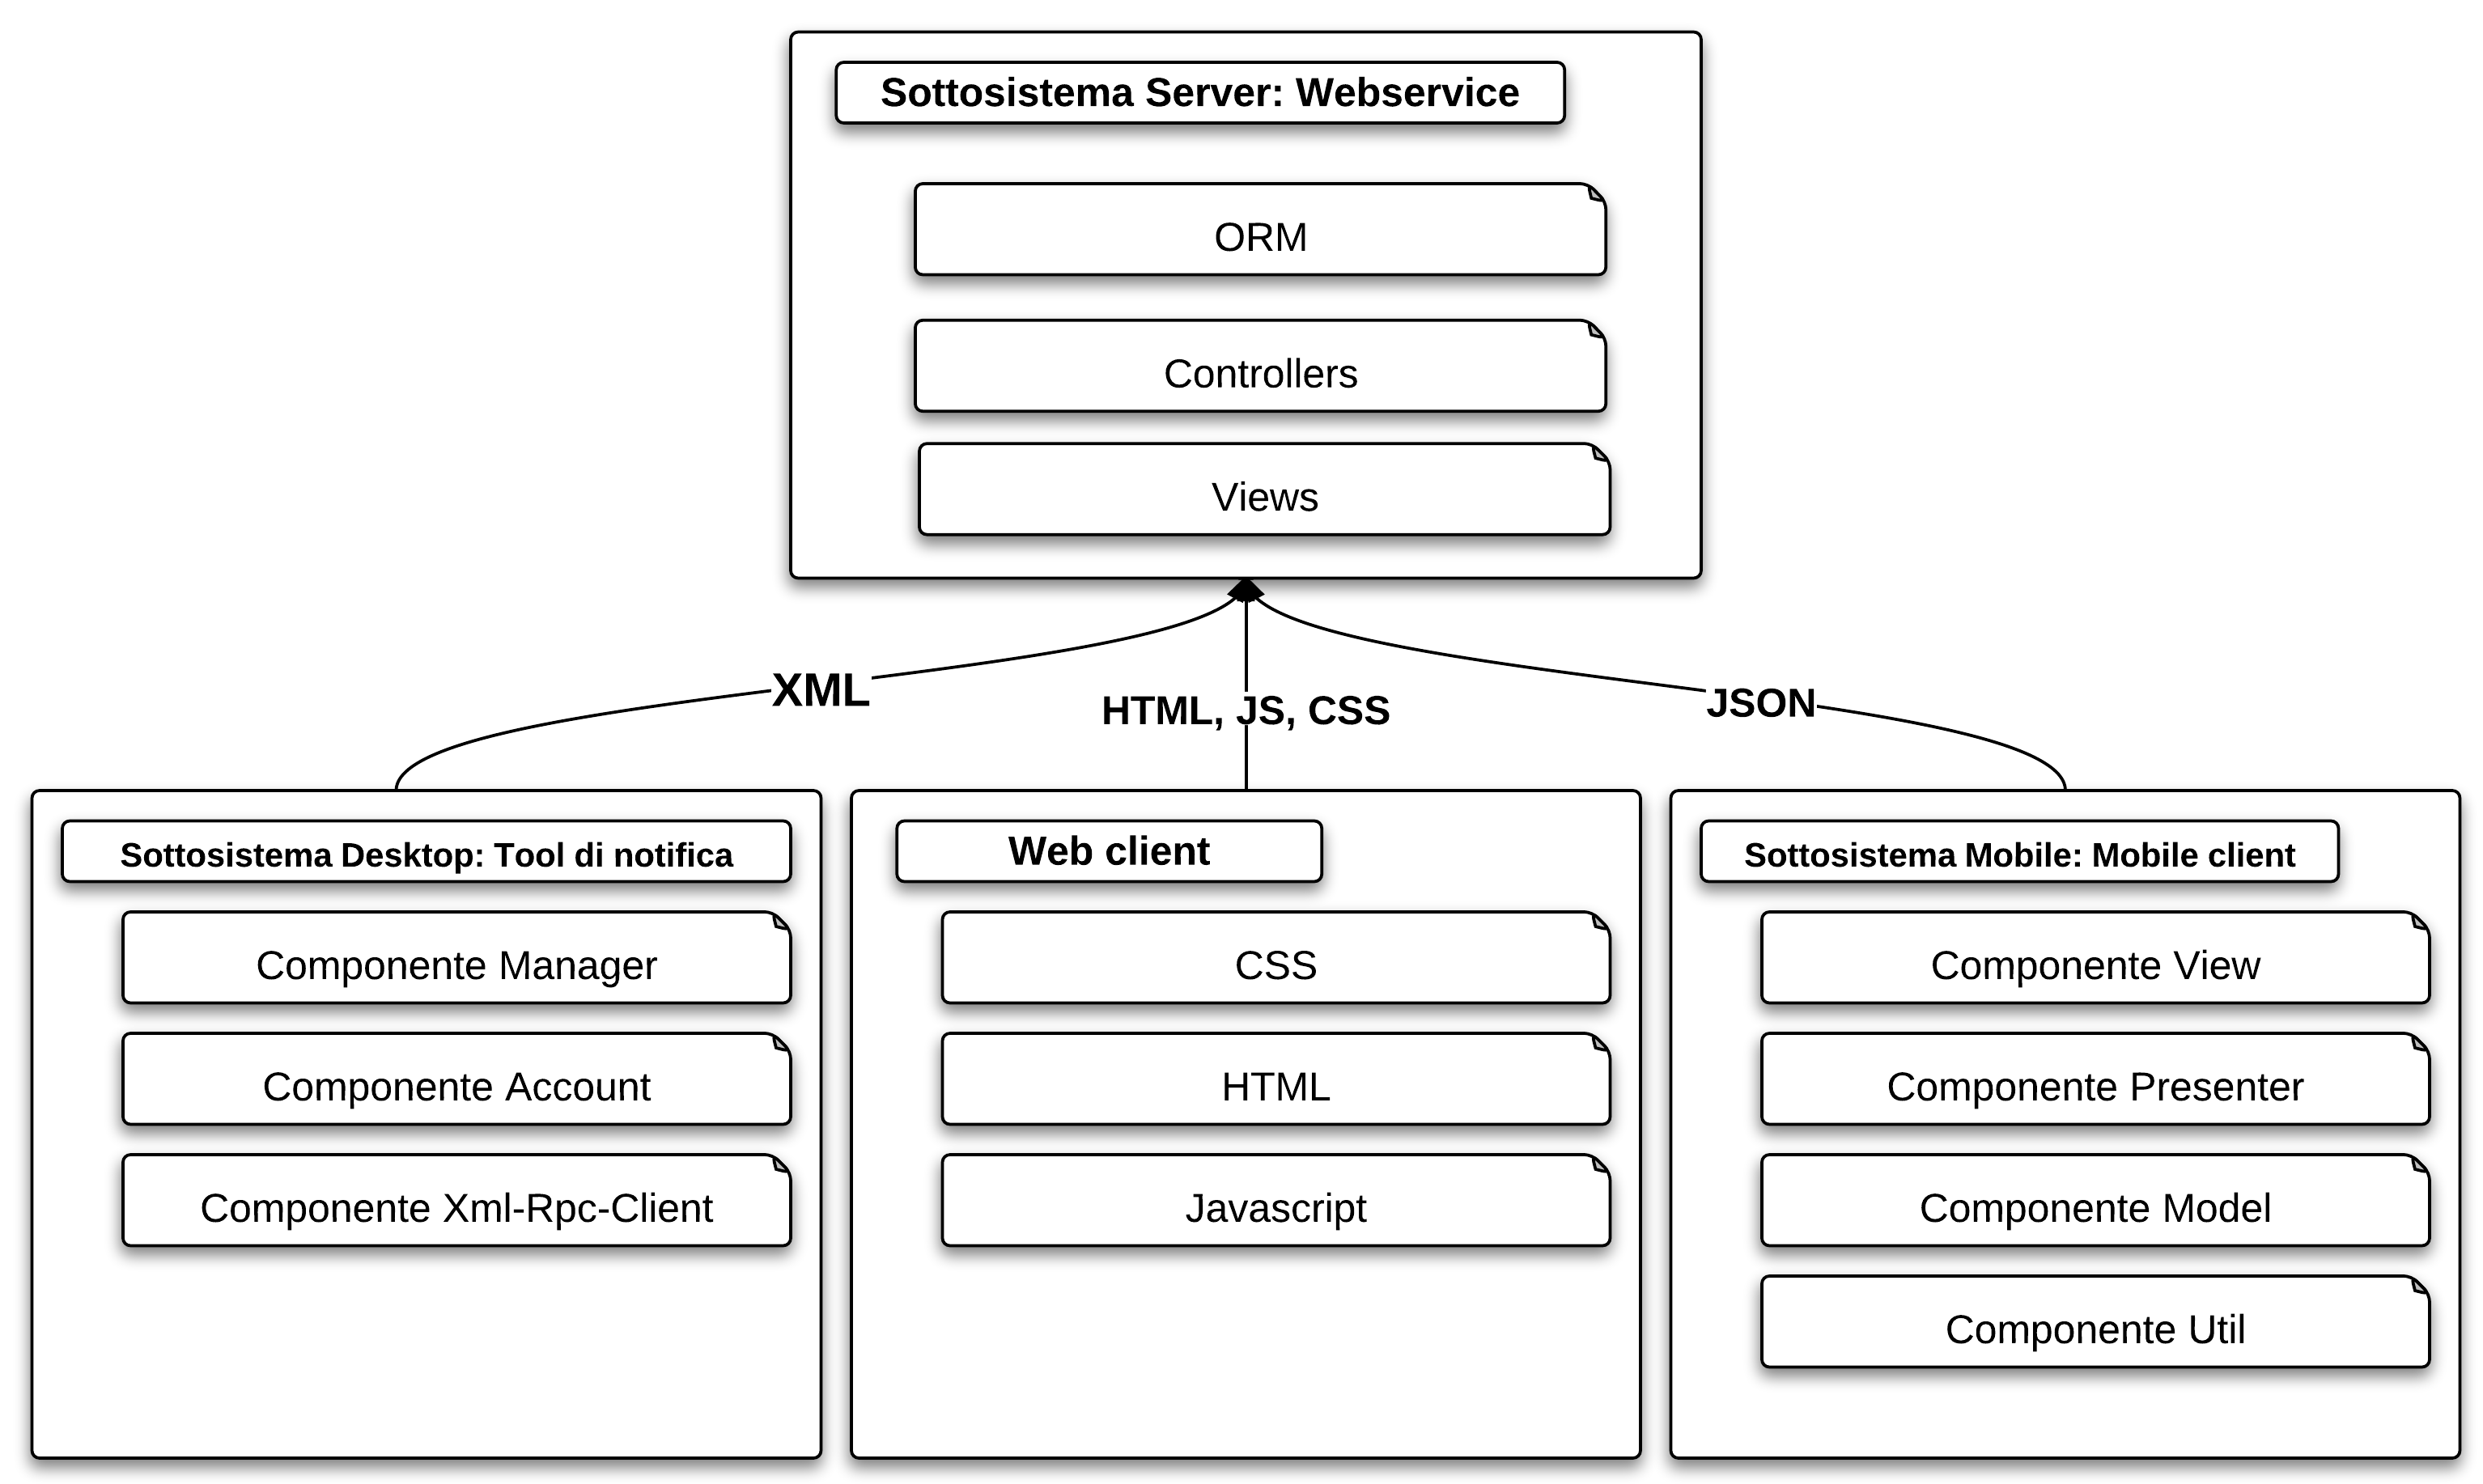
\includegraphics[scale=0.6]{images/cap2/sistema.png} % vedi Lateximpazienye pg67
\caption{Struttura generale del sistema}
\label{StrutturaGeneraleSistema}
\end{figure}



\subsection{Sottosistema Server: Webservice}
Il sottosistema server è responsabile della gestione di tutte le risorse di Woty. Si occupa di interagire con i client, della conservazione e elaborazione dei dati. L'interazione con i web client è permessa attraverso la visualizzazione di pagine HTML, coadiuvate da fogli di stile CSS e di linguaggio lato client Javascript. L'interazione con i client mobile e i tool di notifica desktop è realizzata attraverso comunicazione di messaggi XML e JSON.

% inserire una figura
\begin{figure}[H]
\centering
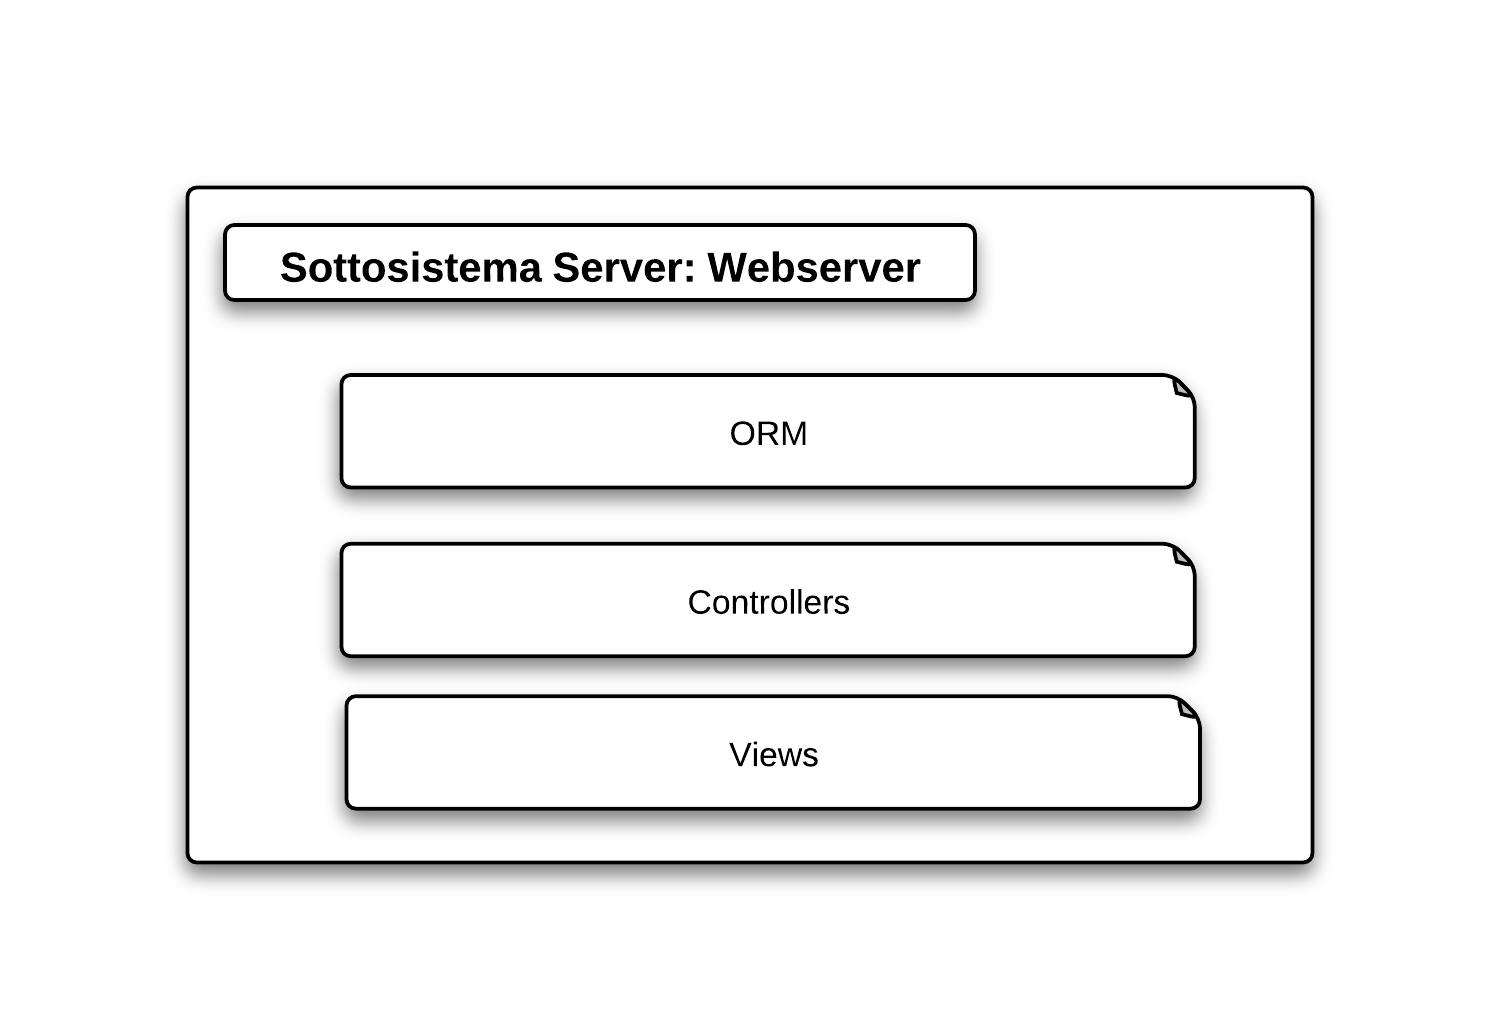
\includegraphics[scale=0.7]{images/cap2/Server/sottosistemaServer.png} % vedi Lateximpazienye pg67
\caption{Sottosistema Server}
\end{figure}

Nel presente documento è presente anche una descrizione più in dettaglio dell'architettura del sottosistema server, in modo da poter comprendere l'interfaccia che il webservice offre all'esterno, oltre che alle logiche interne.


\subsection{Sottosistema Desktop: Tool di notifica}

Il sottosistema Desktop si occupa di gestire la ricezione delle notifiche lato desktop per un utente del tipo Desktop-user, e consiste in una applicazione di tipo Tray Icon semplice ed intuitiva.\\
Una volta installata l'applicazione nell'apposito computer, il Desktop-user potrà effettuare il login al server Woty attraverso le proprie credenziali. In questo modo l'applicazione potrà controllare periodicamente la presenza di nuove quest da svolgere assegnate allo specifico utente, o in caso contrario, l'utente potrà richiederne di nuove.\\
Il sottosistema sarà implementato con l'utilizzo del linguaggio di programmazione object oriented C++, e il framework Qt correlato.\\
Tale sottosistema è stato suddiviso in tre componenti logici come illustrato nella figura \ref{Sottosistema Desktop}.


% inserire una figura
\begin{figure}[H]
\centering
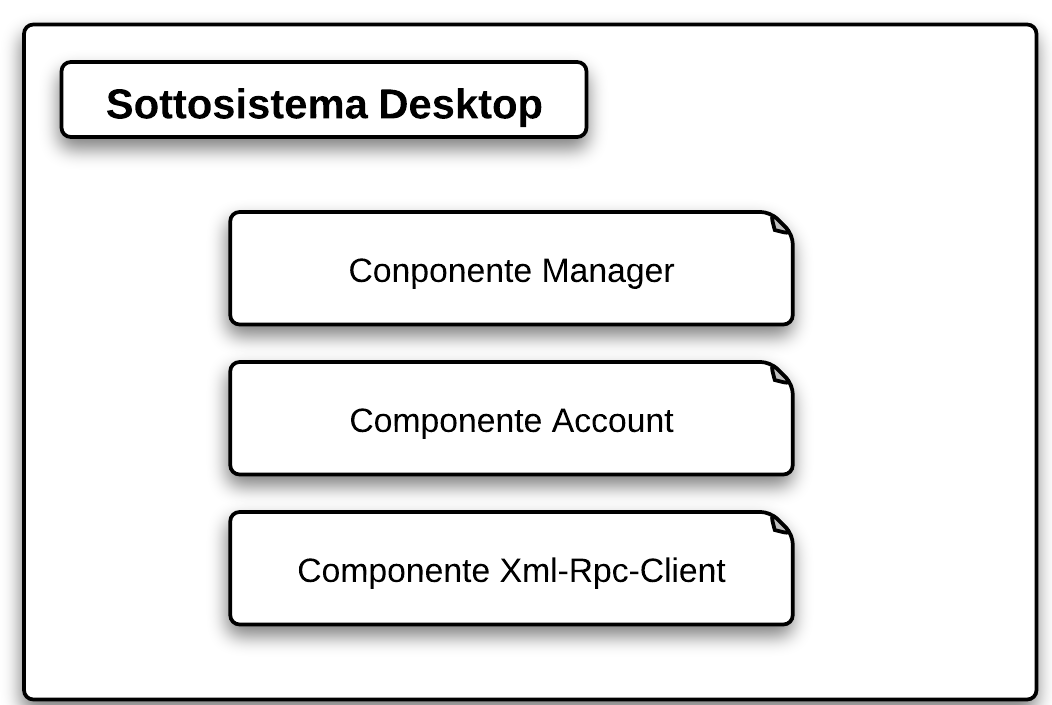
\includegraphics[scale=0.7]{images/cap2/Desktop/sottosistemaDesktop.png} % vedi Lateximpazienye pg67
\caption{Sottosistema Desktop}
\label{Sottosistema Desktop}
\end{figure}



\subsection{Sottosistema Mobile: Mobile client}
Il sottosistema mobile prevede lo sviluppo di un applicazione dedicata per il sistema operativo Android che offra all'utente un' esperienza di navigazione alla pari, o più simile possibile, a quella offerta da una postazione fissa.\\
Questo sottosistema prevede l'interazione con il server per il recupero di tutte le informazioni necessarie e offre un servizio di notifiche push per la segnalazione della presenza di nuove Quest disponibili all'utente autenticato dal dispositivo mobile.\\
Per lo sviluppo architetturale abbiamo scelto di seguire il design pattern MVP, per una massima separazione ed estendibilità del codice.\\
Sono quindi stati previsti i seguenti componenti principali:
\begin{itemize}
\item Componente Model, che rappresenta i dati gestiti dall'applicazione.
\item Componente View, che consiste nelle classi che gestiscono l'interfaccia grafica proposta all'utente.
\item Componente Presenter che è incaricato di gestire le interazioni tra View e Model, in particolare riceve le notifiche generate dell'interazione dell'utente con l'interfaccia grafica e porta a termine le dovute funzioni tramite l'interazione con il Model.
\end{itemize}
Prevediamo poi l'utilizzo di package di supporto come util ed exceptions che forniscono funzionalità come quelle necessarie al parser e alla gestione delle eccezioni. Abbiamo ritenuto di separare questi componenti dal resto della struttura perché non appartengono al design pattern MVP.

% inserire una figura
\begin{figure}[H]
\centering
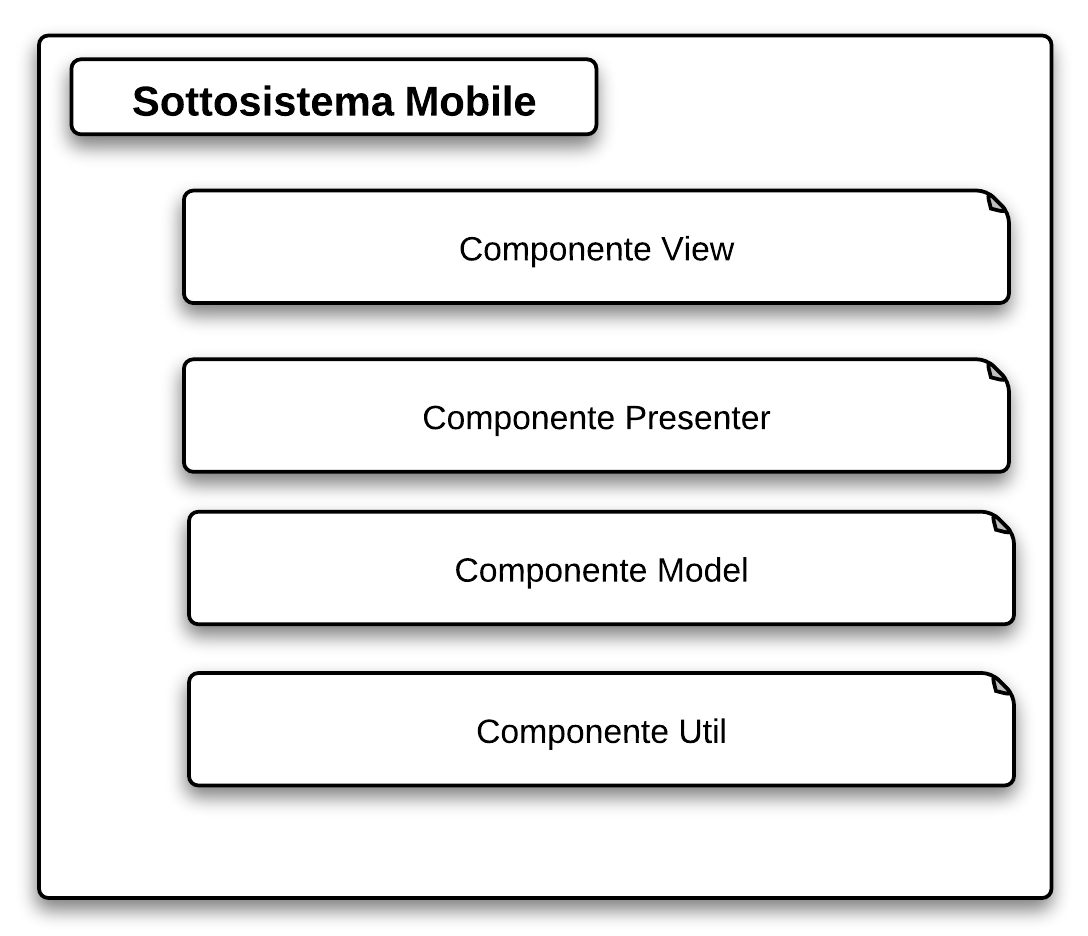
\includegraphics[scale=0.7]{images/cap2/Mobile/sottosistemaMobile.png} % vedi Lateximpazienye pg67
\caption{Sottosistema Mobile}
\end{figure}


\subsection{Web client}
Il web client è un'interfaccia modulare per l'accesso e la modifica dei contenuti utente. Abbiamo identificato due tipologie di pagine web:

\begin{itemize}
\item Pagine di accesso alle risorse, derivate dalle necessità CRUD
\item Pagine statiche, derivate da altri requisiti (es. informazioni del software)
\end{itemize}

Le prime saranno uniformate rispetto ad ogni tipo di risorsa. Le seconde invece avranno layout e contenuti diversi. Riteniamo molto importante la fluidità e l'esperienza d'uso utente. Perciò ci avvaliamo di librerie esterne sicure per fogli di stile e javascript per il buon funzionamento cross-browser e il gusto visivo. Per le stesse ragioni in particolare Ajax ed elementi dinamici saranno utilizzati per simulare la responsività di una vera applicazione locale.

\section{Architettura sottosistema Server}

\subsection{Modalità di descrizione}
Nella presente sezione non verrà descritta ogni classe nel dettaglio, ma verrà utilizzato un approccio più ad alto livello, orientato alle funzionalità che il webservice offre verso l'esterno.
Le richieste esterne verranno effettuate attraverso l'interfaccia REST precedentemente specificata. Le richieste, quindi, saranno tutte verso risorse disponibili nel webservice. \\
Per questo motivo i diagrammi che seguono saranno orientati alla \emph{risorsa}, le varie classi rappresenteranno una classe logica per le risorse e per le risposte che il webservice può dare ad un generico client.

\subsection{Diagramma delle classi}

\subsubsection{HttpResponse}

\begin{figure}[H]
\centering
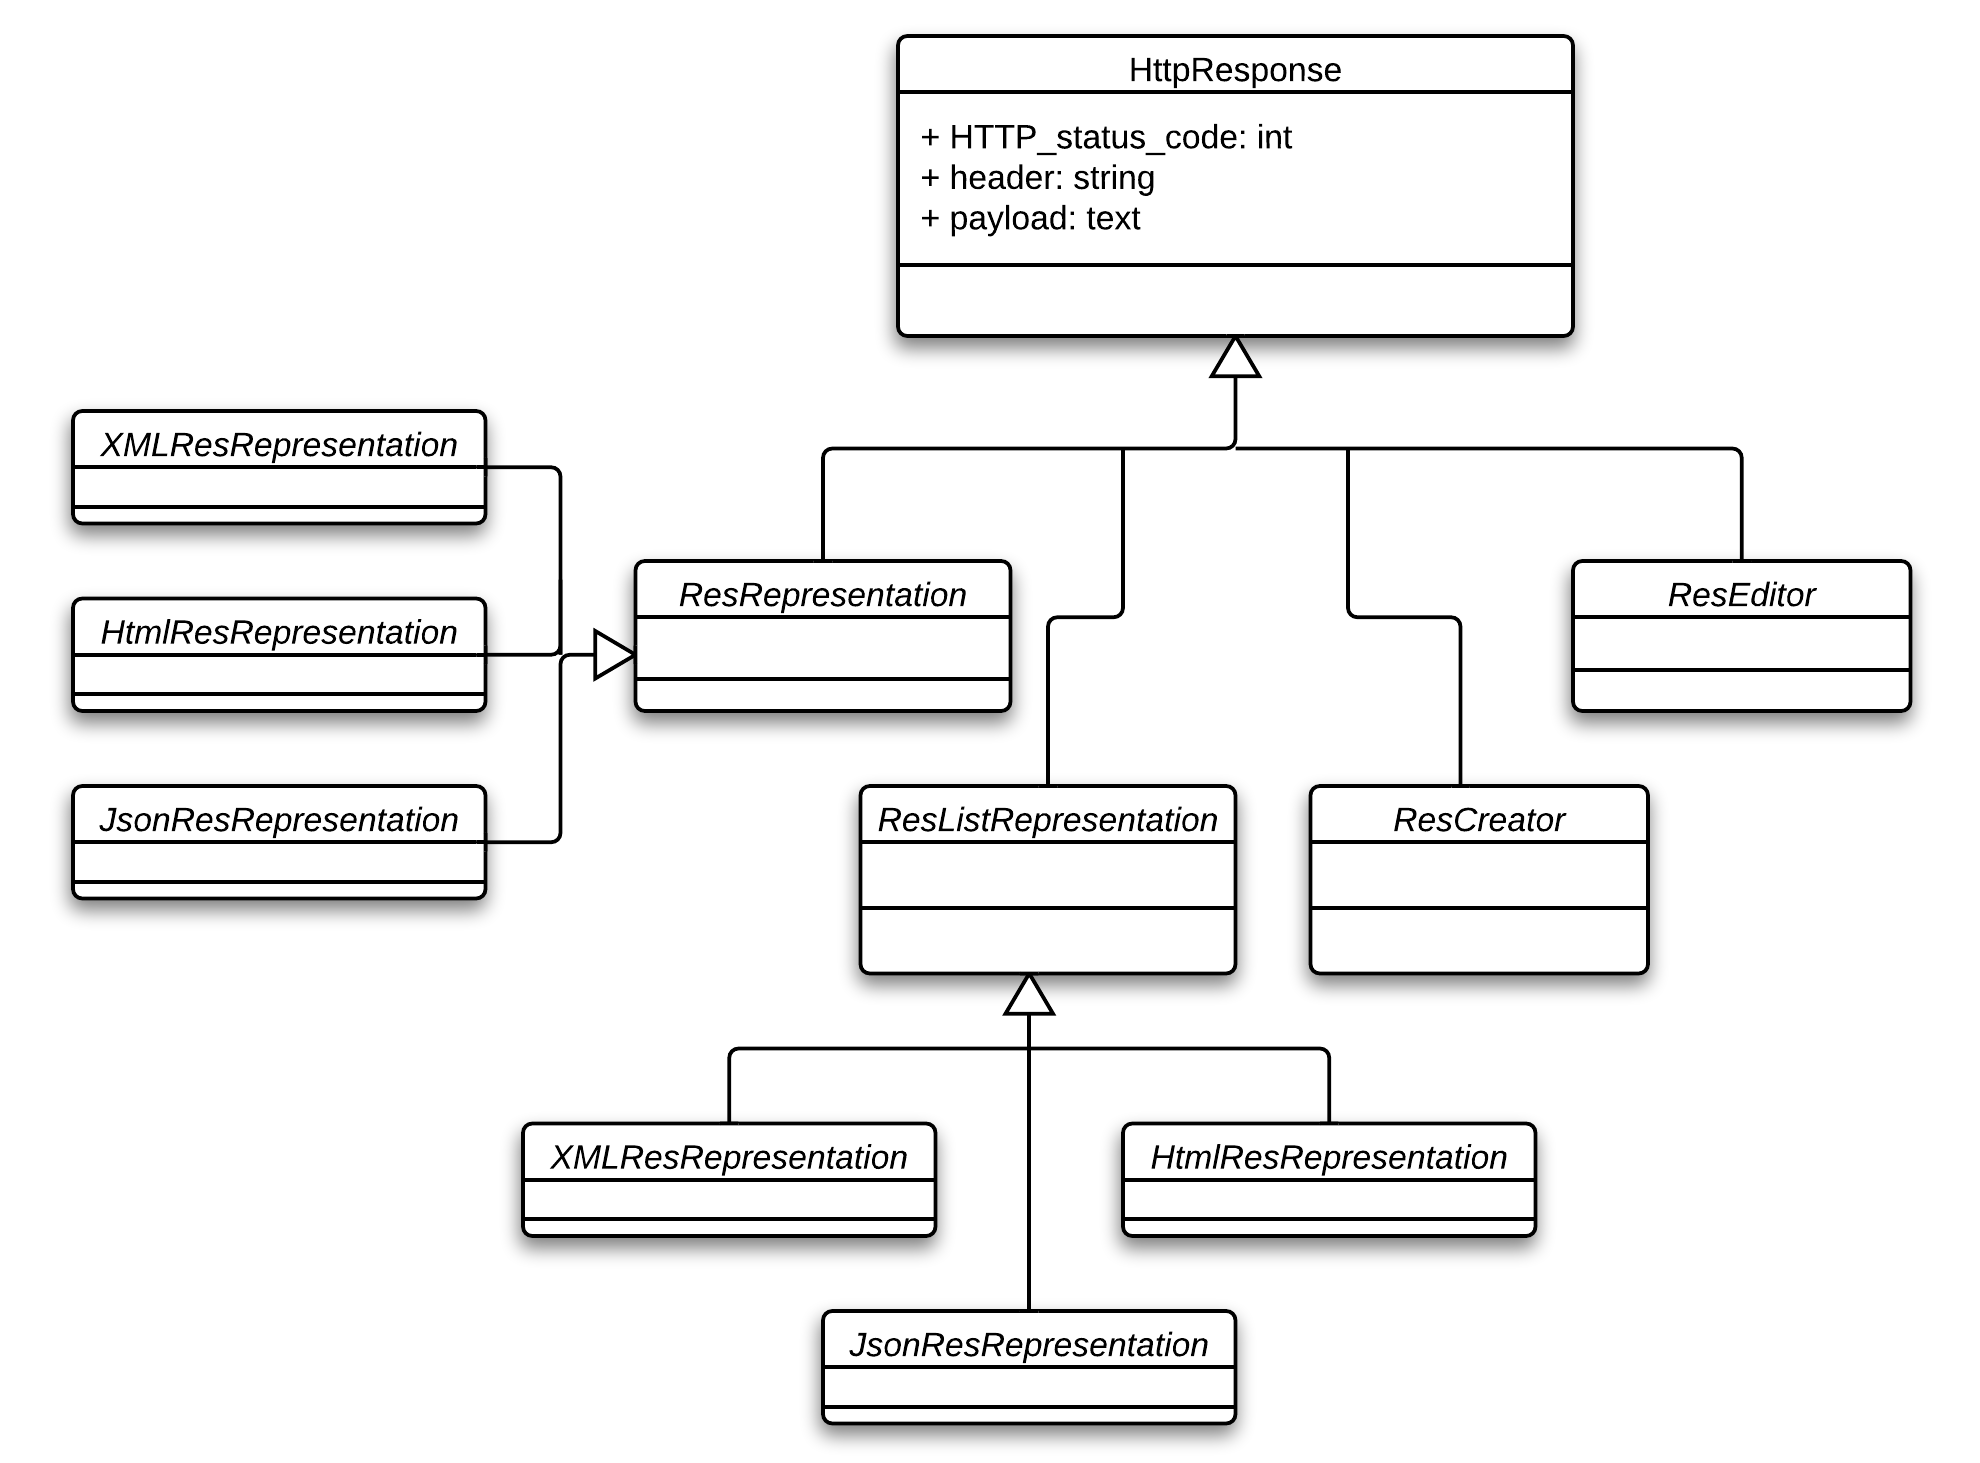
\includegraphics[scale=0.55]{images/cap2/Server/HttpResponse.png}
\caption{Server - HttpResponse}
\end{figure}

Lo scopo del diagramma è il presentare le risposte che il webservice può dare ad un generico client. Di seguito la descrizione delle classi:

\begin{itemize}
\item Classe HttpResponse: rappresenta la risposta HTTP che il webservice restituisce in seguito ad una richiesta REST. E' idealmente caratterizzata da 3 attributi:
\begin{itemize}
\item HTTP\_status\_code: è un intero che rappresenta l'esito della richiesta (e.g. 201 = Created, 401 = Unauthorized)
\item header: contiene meta-informazioni sul contenuto del payload
\item payload: è l'effettivo messaggio trasmesso tramite HTTP 
\end{itemize}
\item Classe ResEditor: è una HttpResponse contenente una vista HTML con la quale è possibile modificare i campi di una risorsa. Genericamente, una form.
\item Classe ResCreator: è una HttpResponse contenete una vista HTML con la quale è possibile creare una risorsa. Anche in questo caso, genericamente è una form.
\item Classe ResListRepresentation:  è una HttpResponse contente lista di istanze di una generica risorsa. Da essa ereditano le classe XMLResListRepresentation, HtmlResListRepresentation, JsonResListRepresentation le quali incapsulano la lista in, rispettivamente, XML, HTML, JSON.
\item Classe ResRepresentation: è una HttpResponse contenete una vista HTML che visualizza una risorsa.Da essa ereditano le classe XMLResRepresentation, HtmlResRepresentation, JsonResRepresentation le quali incapsulano la risorsa in, rispettivamente, XML, HTML, JSON.
\end{itemize}

\subsubsection{Resource}
\label{resource}

\begin{figure}[H]
\centering
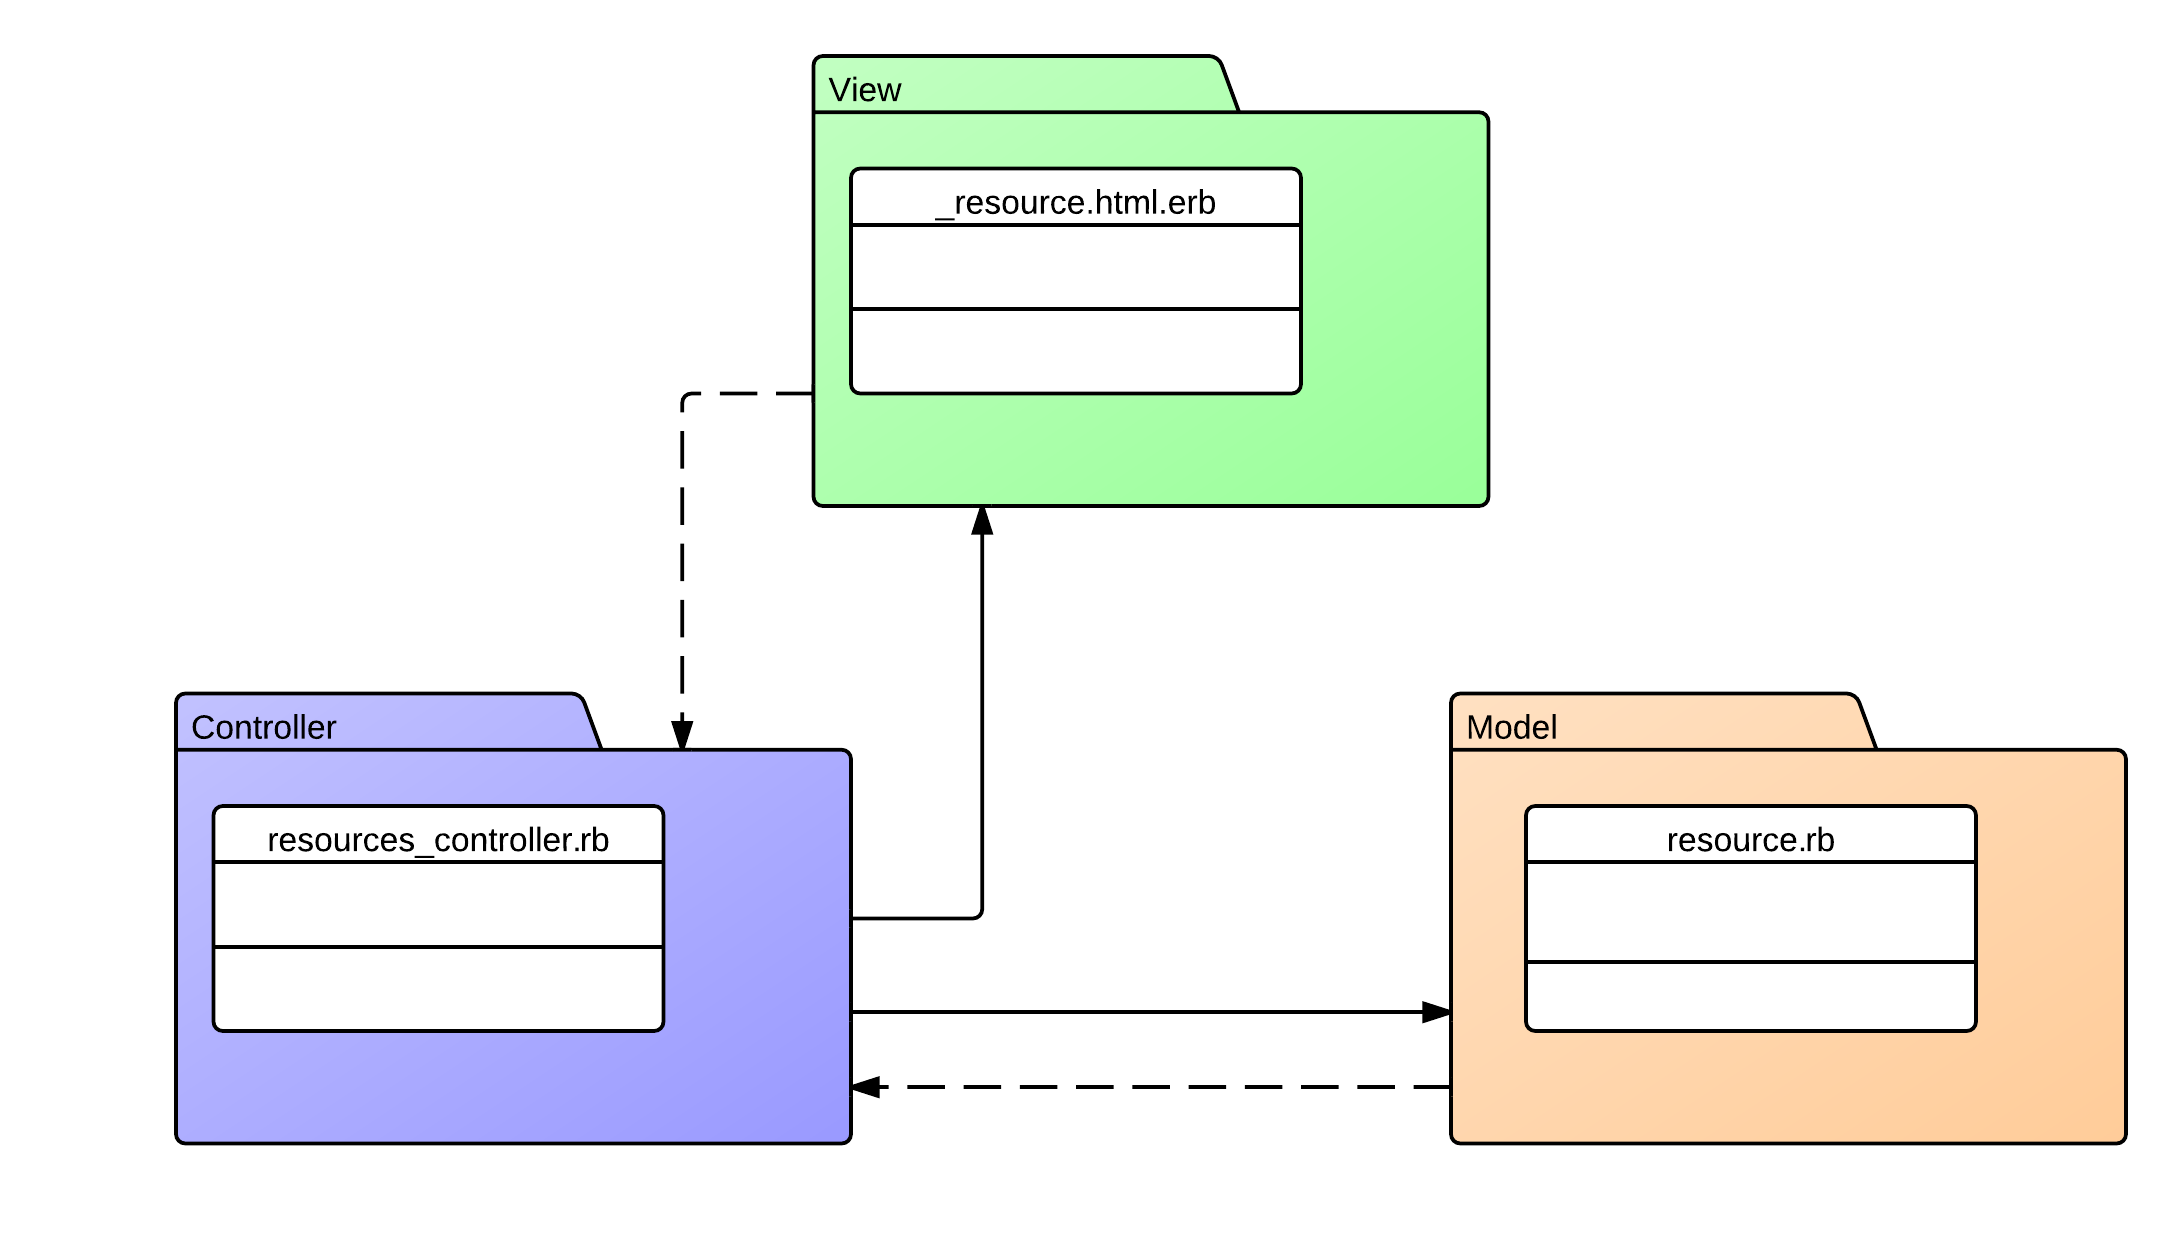
\includegraphics[scale=0.70]{images/cap2/Server/MvcResource.png}
\caption{Server - Resource generica}
\end{figure}

Nel diagramma è rappresentato come è mappata una resource generica secondo il modello model-view-controller del framework RoR.

\begin{figure}[H]
\centering
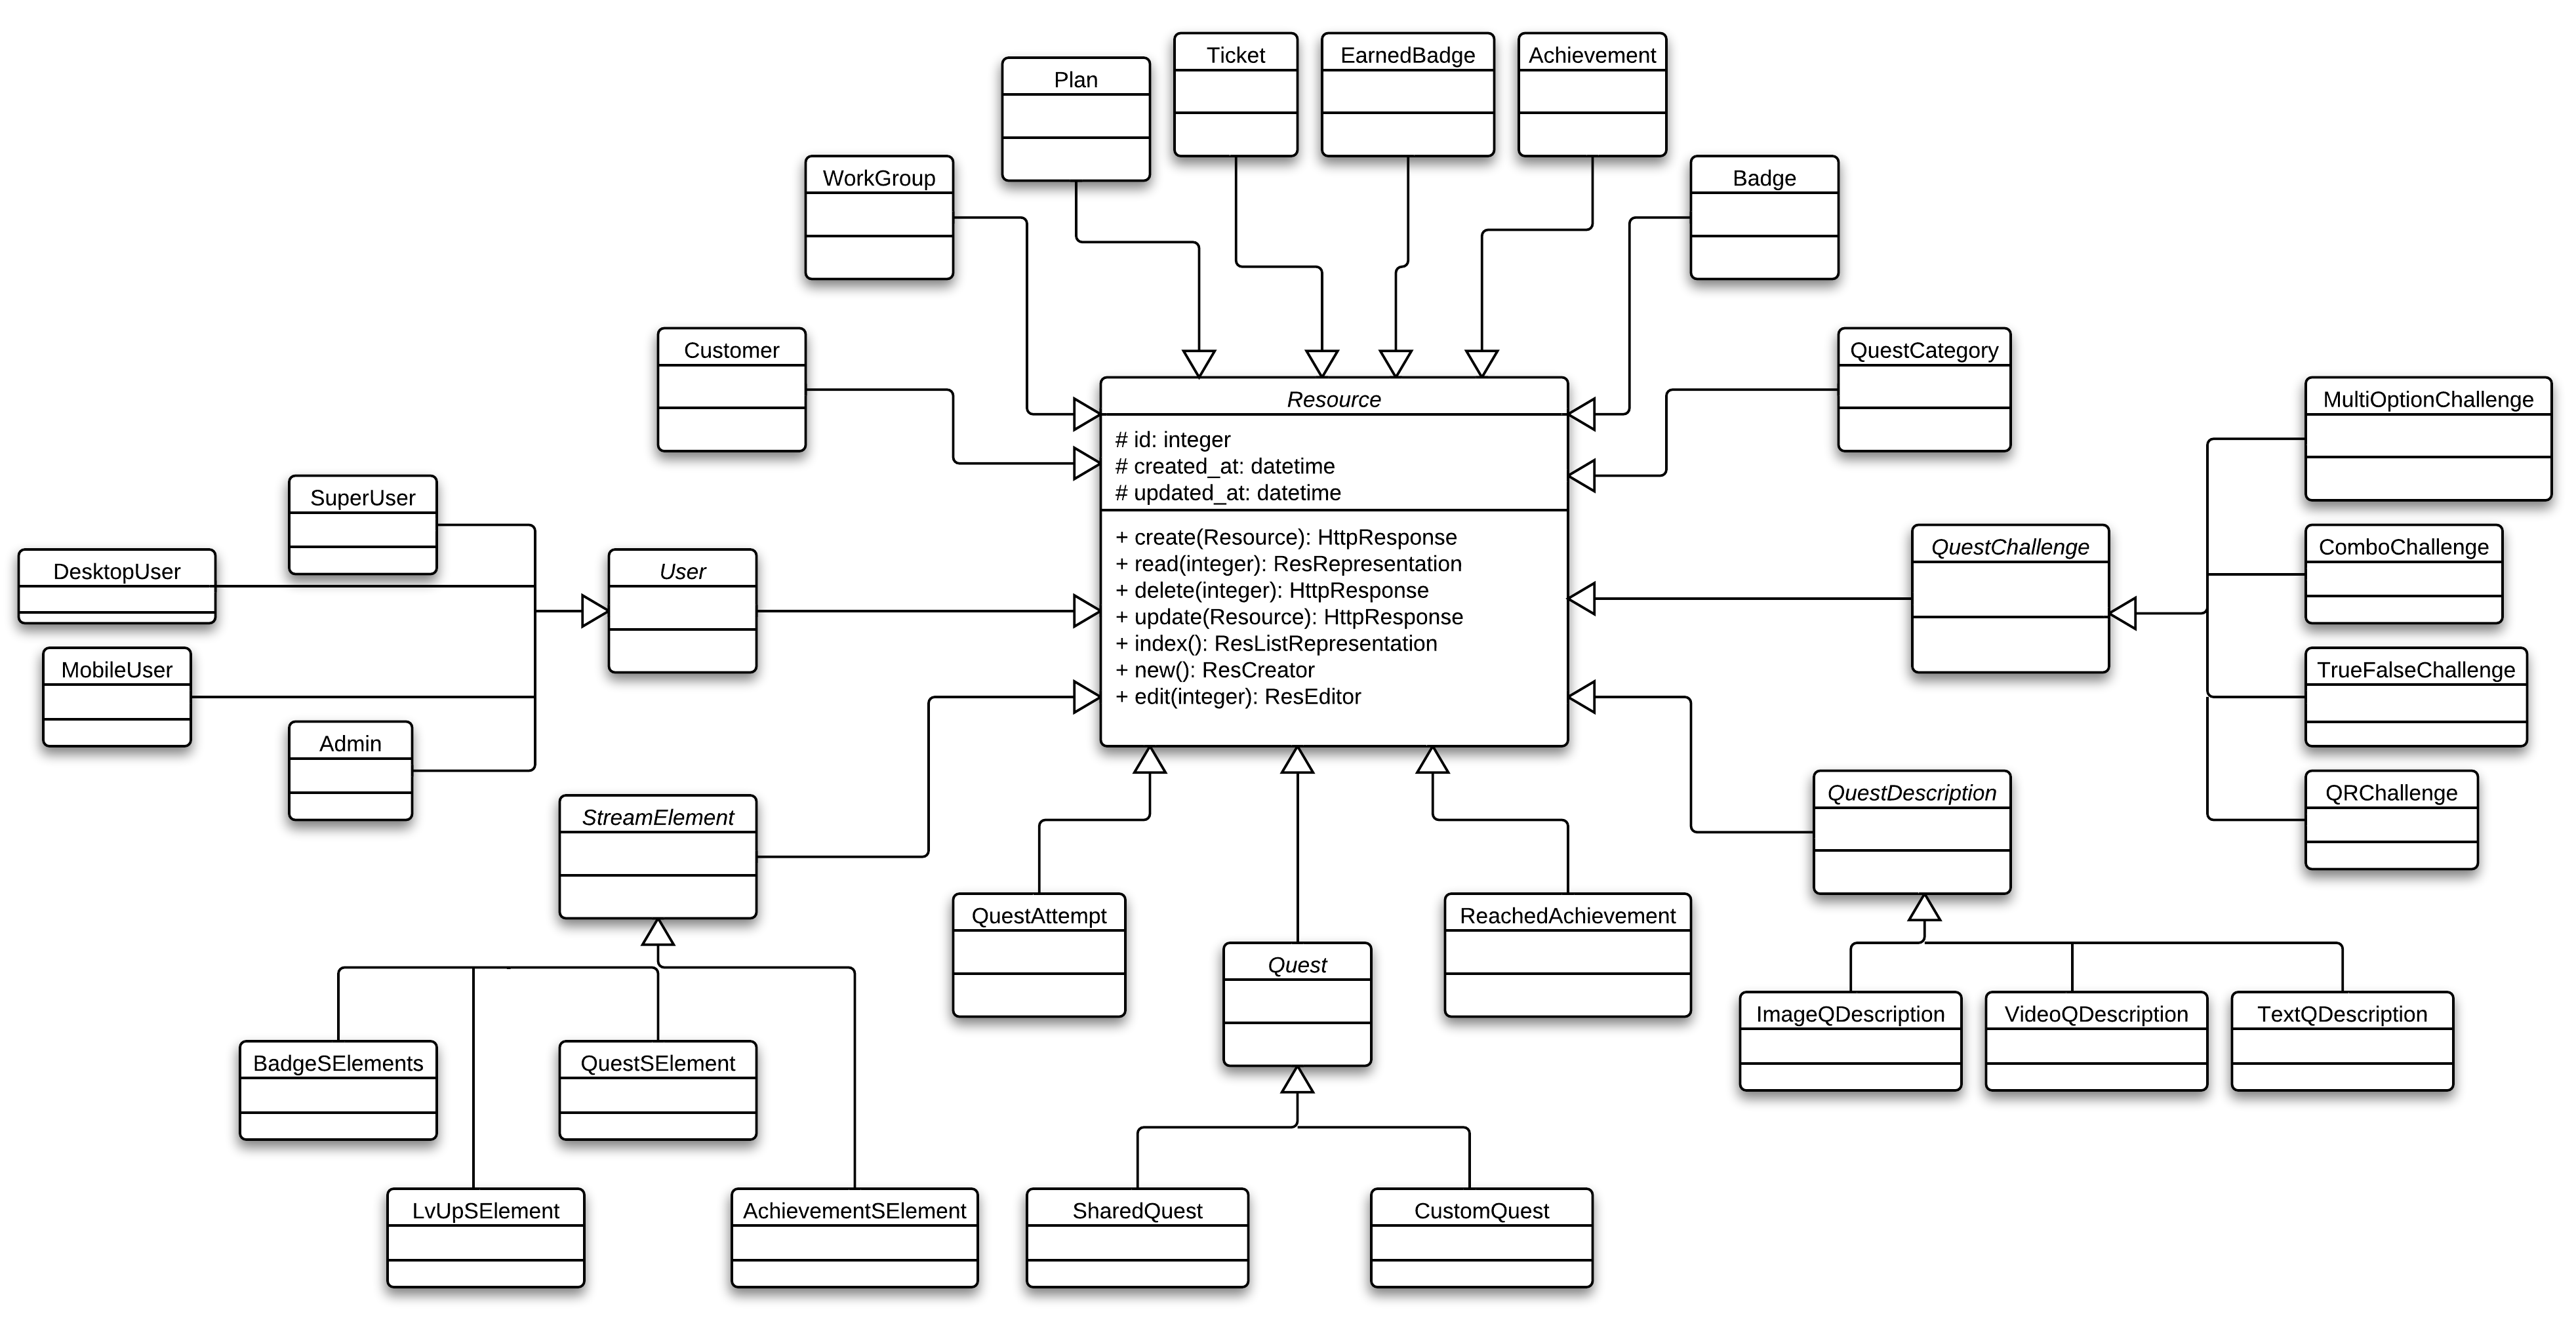
\includegraphics[scale=0.50]{images/cap2/Server/Resource.png}
\caption{Server - Resource}
\end{figure}

Questo diagramma vuole mostrare come ogni classe logica disponibile nel webservice sia in realtà una risorsa. Le relazioni e le dipendenze più dettagliate tra le classi saranno visibili in seguito nel diagramma degli oggetti in figura \ref{S-do}.\\


\subsubsection{Diagramma ad oggetti}
Il seguente diagramma ad oggetti vuole mettere in evidenza come una risorsa sia effettivamente una tabella nel DB, e le relazioni tra le varie risorse.

\begin{figure}[h]
\centering
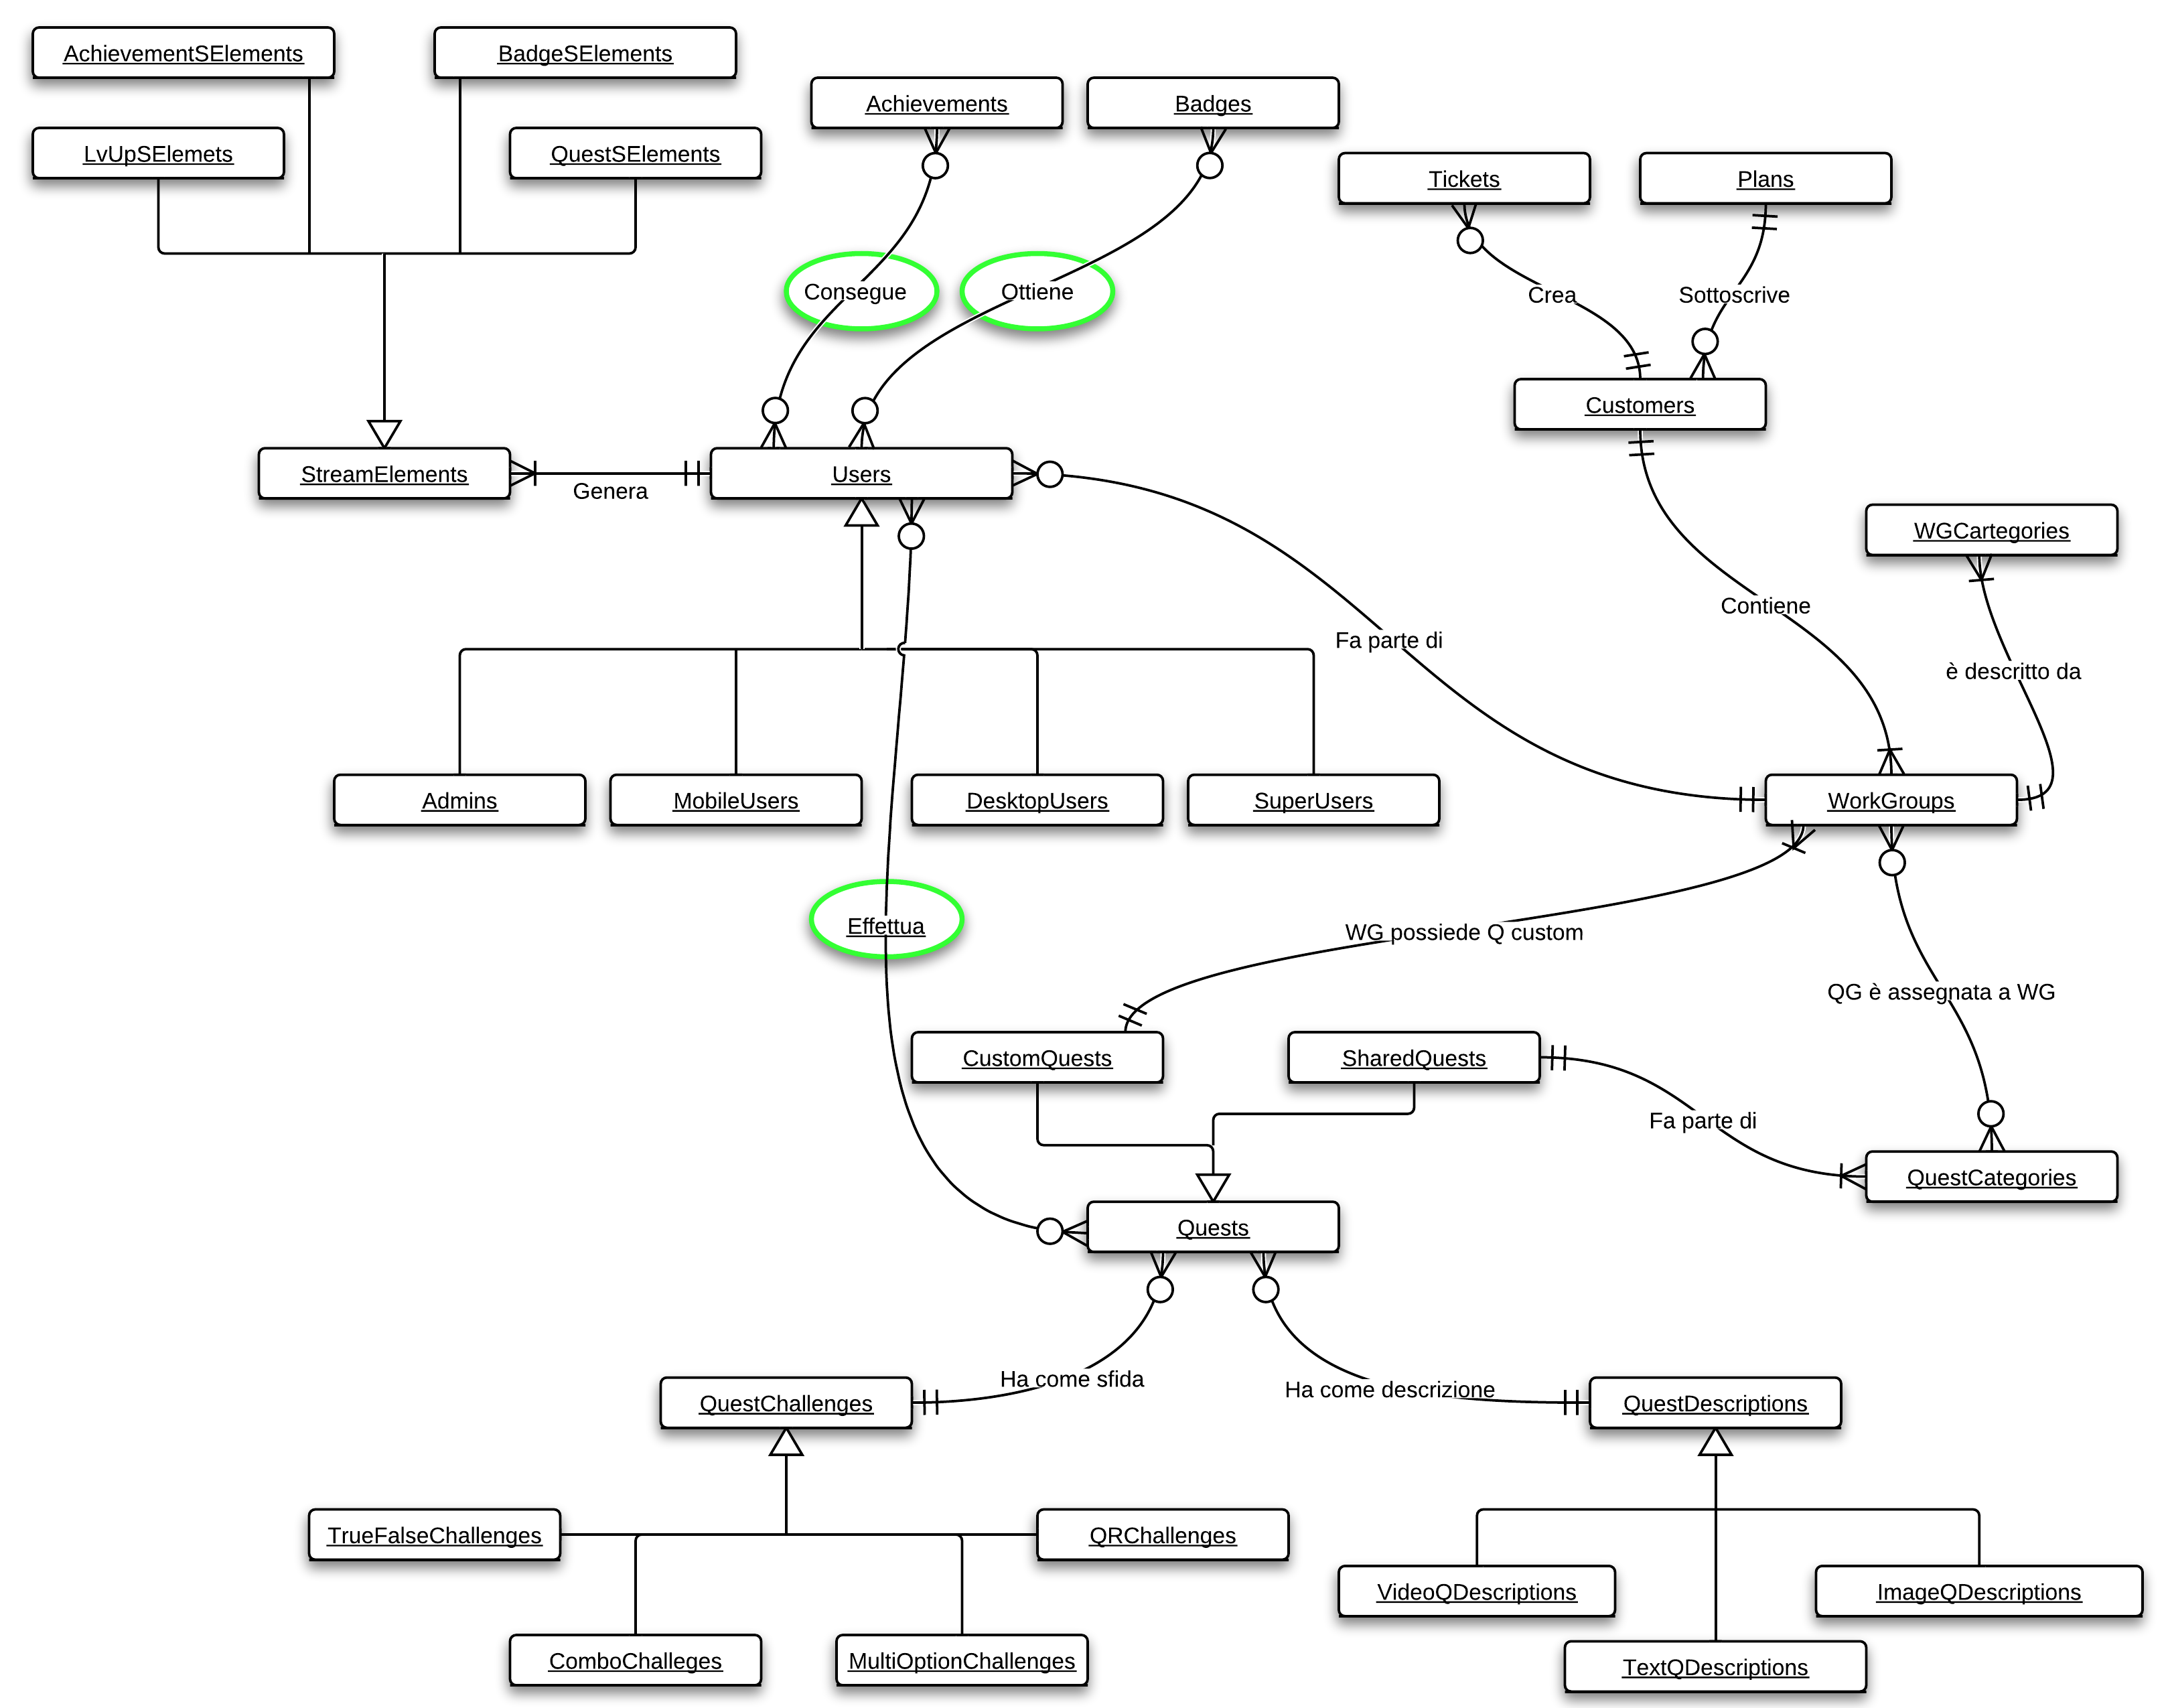
\includegraphics[scale=0.55]{images/cap2/Server/Oggetti.png}
\caption{Server - Diagramma ad oggetti}
\label{S-do}  % S-do = Server - diagramma oggetti
\end{figure}

Da notare il fatto che dalle relazioni N:M nascano delle risorse:

\begin{itemize}
	\item Dalla relazione Users <-> Quests nasce la risorsa QuestAttempt.
	\item Dalla relazione Users <-> Achievements nasce la risorsa ReachedAchievent.
	\item Dalla relazione Users <-> Badge nasce la risorsa EarnedBadge.
\end{itemize}

Altri punti che meritano una spiegazione:

\begin{itemize}
	\item Dalla relazione N:M WorkGroups <-> QuestCategories è stato deciso di non far emergere una risorsa, seppur una tabella debba necessariamente essere creata.
	\item L'entità WGCategories è una tabella nata per evitare ridondanze nella denominazione dei WorkGroup, non è stato quindi ritenuto necessario mapparla come risorsa.
\end{itemize}

\subsection{Descrizione risorse}
Verrà di seguito riportata una descrizione delle risorse di Woty, in modo da poter meglio comprendere cosa rappresentano e quali relazioni presentano tra di esse

\subsubsection{User} Utente base registrato al sistema. Classe base della gerarchia di utenti.
\subsubsection{SuperUser} Utente con privilegi di SuperUser
\subsubsection{DesktopUser} Utente Desktop
\subsubsection{MobileUser} Utente Mobile
\subsubsection{Admin} Amministratore di Woty
\subsubsection{Customer} Risorsa che modella i clienti del fornitore del servizio. Ogni customer ha vari workgroup che a loro volta contengono una serie di user. Ogni customer inoltre sottoscrive un plan, che definisce il livello di servizio per il customer.\\
Nel sistema è un'entità molto importante in quanto tutti gli utenti fruiscono dei contenuti all'interno del loro customer.\\
\subsubsection{WorkGroup} Classe che rappresenta un reparto di un'azienda cliente, che sono composti dagli utenti facenti parte dello stesso.\\
Gli utenti in reparti lavorano anche in team, e sono disponibili classifiche di reparto. Sono inoltre utilizzati per l'assegnazione delle quest, in quanto il reparto è una delle caratteristiche per le quali sono influenzate le categorie di rischio.
\subsubsection{Plan}Risorsa che modella le formule d'acquisto del prodotto. Il paradigma Software as a Service uniforma nel miglior modo possibile il maggior numero di clienti.\\
Per il nostro caso possono essere sottoscritti vari piani di acquisto.\\
All'interno del plan sono definite alcune abilità che possono o meno essere utilizzate a seconda del prezzo pagato.
\subsubsection{Quest} La classe modella le quest e la loro composizione. Di fatto le quest sono composte di una descrizione e una sfida: entrambe possono essere di vario tipo e sono rappresentate tramite gerarchie.
Le quest inoltre hanno una categoria che può essere inclusa in un workgroup: gli utenti facenti parte sono in grado di svolgere le quest con le categorie associate.
\subsubsection{QuestDescription}Classe base della gerarchia inerente le tipologie di descrizione di una quest. La gerarchia è utilizzata per la composizione di una quest.
\subsubsection{TextDescription} Rappresenta una QuestDescription che contiene solo testo.
\subsubsection{ImageDescription} Rappresenta una QuestDescription che contiene un'immagine.
\subsubsection{VideoDescription} Rappresenta una QuestDescription che contiene un video.
\subsubsection{QuestChallenge} Classe base per le sfide delle quest. Rappresenta il componente sfida delle quest che può essere di varie tipologie, definite tramite le sottoclassi.
\subsubsection{ComboChallenge} Classe che rappresenta un quesito a risposta multipla con una ed una sola risposta corretta.
\subsubsection{TrueFalseChallenge} La classe modella una tipologia particolare di QuestChallenge contenente più affermazioni, ognuna delle quale può essere vera o falsa.
\subsubsection{MultiOptionChallenge} La classe modella una tipologia particolare di QuestChallenge contenente più affermazioni, ognuna delle quale può essere valida o meno. Si differenzia da TrueFalseChallenge a livello logico, in quanto più che possibili affermazioni che possono essere vere e false, modella possibili opzioni che possono essere valide o meno.
\subsubsection{Achievement} Gli achievement sono modellati tramite una serie di condizioni legate dall'operatore logico AND. Per semplicità di implementazione non si è ritenuta necessaria l'implementazione di altri operatori logici. La validità di un achievement è calcolata per uno user e valida tutte le condizioni associate.
\subsubsection{Like} Like è la risorsa che modella i like effettuati dagli utenti. Attualmente
è possibile effettuare i like solo su elementi membri della gerarchia StreamElement.
\subsubsection{StreamElemet}StreamElement è la classe base per gli elementi di attività visibili nel pannello utente. Le attività possono essere di vario genere, permettono l'interazione tramite like e commenti, e costituiscono il principale elemento social del sistema.
\subsubsection{QuestHistory} Una QuestHistory relaziona uno User con una Quest. Viene creata
quando uno User svolge una Quest oppure quando il sistema assegna ad uno User una Quest.
\subsubsection{Ticket}Rappresenta un Ticket creato da un SuperUser e rivolto al/agli Admin del sistema.
\subsubsection{CompletedAchievement}Rappresenta un achievement ottenuto da un utente.
\subsubsection{CompletedAchievementElement}Specializzazione della classe StreamElement che rappresenta l'ottenimento di un achievement da parte di un utente.
\subsubsection{Condition}La classe modella una condizione necessaria al completamento di un achievement. Le condizioni sono composte da un operatore, uno dei valori definiti in Achievable, e un valore fissato dal creatore. Abbiamo deciso di limitare la libertà di creazione delle condizioni, in quanto altre soluzioni sarebbero state troppo complesse da implementare. Il sistema le rende comunque generabili dinamicamente.
\subsubsection{CustomQuest}Modella una Quest personalizzata, disponibile solo ad un determinato Workgroup
\subsubsection{QuestCategory}Identifica una categoria di rischio al quale una SharedQuest è associata
\subsubsection{SharedQuest}Rappresenta una Quest condivisa tra più Workgroup





% --------------------------------------------------------------------

%####################################################
%   cap Lorenz
%####################################################


\chapter{Pianificazione del lavoro}
\label{pianificazioneDelLavoro}

\section{Introduzione}
Il gruppo di lavoro si trova ad aver progettato e in amplia parte sviluppato il software in questione nell'ambito del progetto del corso di studi Ingegneria del software. \\Per poter procedere ad una fase successiva il team si prefigge l'obiettivo di effettuare una analisi di mercato e un relativo studio di fattibilità per ottenere il via libera per la realizzazione di un prodotto funzionante e la sua commercializzazione.\\In questo documento intendiamo quindi presentare l'elaborato della \virgolette{seconda fase} (vedi capitolo seguente) per riuscire poi a proseguire nella realizzazione del progetto, vediamo in dettaglio la suddivisione del lavoro e lo stato di avanzamento:

\section{Fasi di avanzamento}

\vspace*{0.5cm}

\begin{figure}[H]
\centering
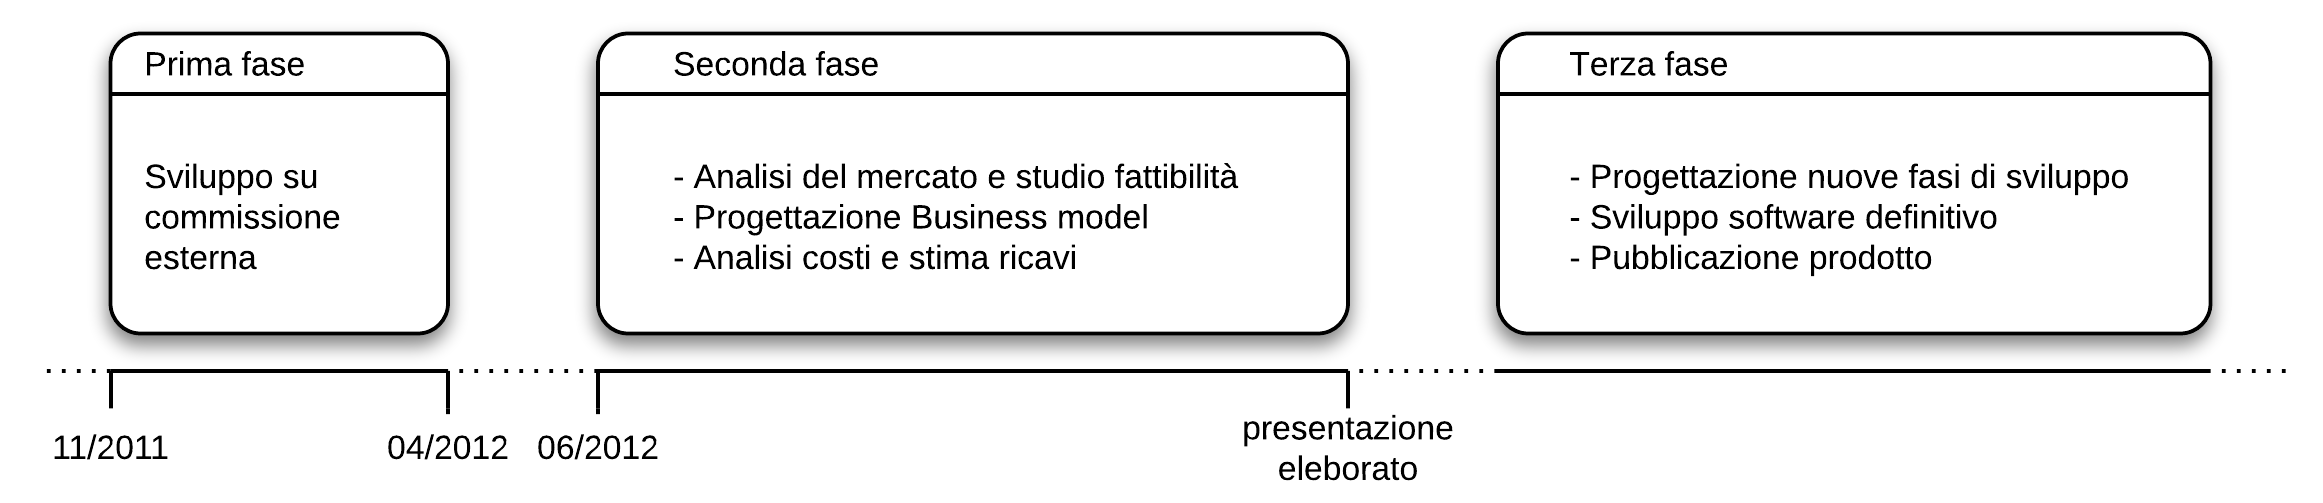
\includegraphics[scale=0.7]{images/cap3/avanzamento.png}
\caption{Avanzamento lavoro}
\end{figure} 

\vspace*{0.5cm}

In figura \virgolette{Avanzamento lavoro} si può vedere l'avanzamento temporale del progetto e la suddivisione in fasi del lavoro del nostro gruppo. È da sottolineare ancora una volta che il presente documento intende presentare i risultati della fase due per proporre l'avanzamento del progetto alla sua fase conclusiva. Vediamo formalmente la divisione in fasi: \\

\begin{itemize}
\item Prima fase (corso Ingegneria del software):
\begin{itemize}
\item Sviluppo su commissione esterna 
\end{itemize}
\end{itemize}

\begin{itemize}
\item Seconda fase (presentata in questo documento):
\begin{itemize}
\item Analisi del mercato e studio fattibilità
\item Progettazione Business model
\item Analisi costi e stima ricavi
\end{itemize}
\end{itemize}

\begin{itemize}
\item Terza fase (all'approvazione della fase due):
\begin{itemize}
\item Progettazione nuove fasi di sviluppo
\item Sviluppo software definitivo
\item Pubblicazione prodotto
\end{itemize}
\end{itemize}

\newpage

\section{Fase due: strumenti e risorse}
Per affrontare con massima efficienza la fase due del progetto il nostro team di lavoro deve avvalersi di alcune risorse, sia intese come strumenti per facilitare il lavoro, sia come conoscenze che i componenti del gruppo hanno già in parte apprese dal corso di Sviluppo e Gestione dei Progetti e devono mettere in pratica. In questo capitolo vediamo come si intende affrontare questa fase, quali strumenti intendiamo utilizzare per garantire un alta qualità del lavoro e quali figure ci sono indispensabili per raggiungere un livello di dettaglio adeguato.

\subsection{Strumenti}
\begin{itemize}
\item Git: software per il versionamento del documenti, essenziale al nostro team per poter lavorare liberamente su documenti senza rischiare di perdere avanzamenti importanti svolti da altri componenti del gruppo.
\item Teamspeak: software per la comunicazione vocale tramite la rete internet che ci permette di compiere meno movimenti sul territorio e poter svolgere comunque il nostro lavoro. Tuttavia non sarà uno strumento sufficiente per eliminare gli incontri settimanali organizzati dal gruppo per aggiornare lo svolgimento e discutere gli eventuali problemi riscontrati.
\item Google Drive: utility offerta da google per la condivisione di documenti sui quali lavorare in modo concorrente e in tempo reale.
\item Editor LaTex: software che permette la stesura di documenti in modo formale e pulito. Verrà utilizzato per la scrittura e l'impaginazione di tutti i documenti ufficiali in questo progetto.
\end{itemize}

\subsection{Figure}
In figura \virgolette{Organization Breakdown Structure} è mostrata l'organizzazione adottata dal team per ottenere una migliore gestione carico di lavoro. È essenzialmente un'organizzazione a matrice debole, che vede il Capo progetto come Project Manager e Come Manager di Funzione i vari esperti e capi. Vediamo ora lo schema e la descrizione di ogni ruolo:

\vspace*{0.5cm}

\begin{figure}[H]
\centering
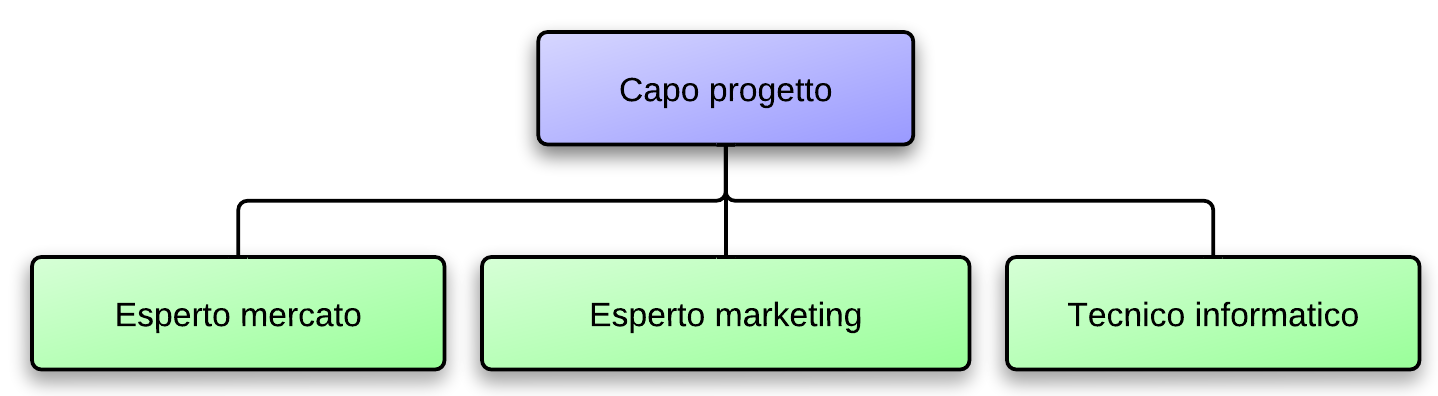
\includegraphics[scale=1]{images/cap3/obs.png}
\caption{Organization Breakdown Structure}
\end{figure}

\vspace*{0.5cm}

\begin{itemize}

\item Capo progetto: ha il compito di pianificare e monitorare le attività del team. Parteciperà inoltre attivamente alle principali fasi di analisi e progettazione tra cui l'analisi del prodotto, lo studio di fattibilità, la realizzazione del business model e alle stime di rischi e costi.

\item Esperto sicurezza: ha il compito di studiare il mercato in cui vorremmo introdurre il nostro prodotto. Oltre all'analisi di mercato, segue lo studio della concorrenza e partecipa allo studio di fattibilità e alla realizzazione del business model portando in ingresso a questa fase i dati raccolti dai precedenti studi. 

\item Esperto marketing: ha il compito di studiare la campagna pubblicitaria del nostro prodotto e parteciperà quindi allo studio di fattibilità e alla realizzazione del business model trattando principalmente la sezione dei channels.

\item Tecnico informatico: consulente che offre le sue conoscenze durante le attività dello studio di fattibilità, realizzazione business model e stime di rischi e costi. Può aiutare a quantificare gli investimenti necessari a realizzare l'infrastruttura IT del prodotto e calcolarne i costi gestione/manutenzione. Può inoltre preventivare i costi necessari ad apportare modifiche al software.

\end{itemize}

\subsection{Responsabilità}
Da sottolineare il fatto che queste figure possono essere ricoperte da più persone sia contemporaneamente che in momenti diversi, e di tutto il loro lavoro sarà tenuta traccia sotto forma di documentazione.
Le responsabilità che ogni figura ha sull'elaborato sono mostrate in figura \virgolette{Responsabilità} e indicano il peso delle decisioni di ogni figura sul lavoro che sta supervisionando o svolgendo:

\vspace*{0.5cm}

\begin{figure}[H]
\centering
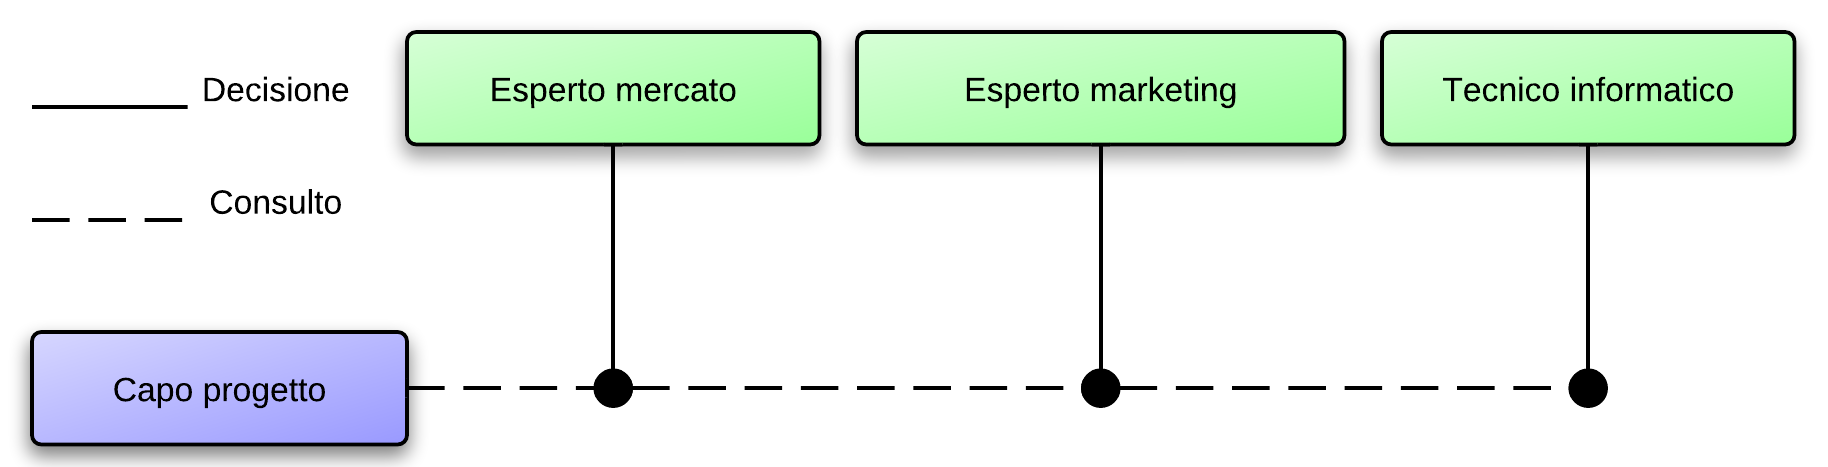
\includegraphics[scale=0.8]{images/cap3/resp.png}
\caption{Responsabilità}
\end{figure}

\vspace*{0.5cm}

Possiamo vedere nel diagramma \virgolette{Responsabilità} come il capo progetto abbia potere di consulenza e supervisione su tutte le parti del gruppo di lavoro, ma che l'aspetto decisionale spetti direttamente al responsabile di quella attività.

\newpage

\section{Pianificazione temporale}

Il nostro team per garantire un adeguata qualità del lavoro si impegna a seguire uno schema temporale che ricopre tutto lo svolgimento della fase due del progetto, quindi ogni figura deve svolgere delle attività prestabilite seguendo un calendario preciso. \\Ogni discrepanza con le tempistiche da parte di uno qualsiasi dei membri del gruppo può e deve essere affrontata sotto la diretta supervisione del capo progetto, che di volta in volta dovrà decidere come precedere per risolvere il problema. \\Vediamo ora in figura \virgolette{Gantt} la schedulazione prevista:

\vspace*{0.5cm}

\begin{figure}[H]
\centering
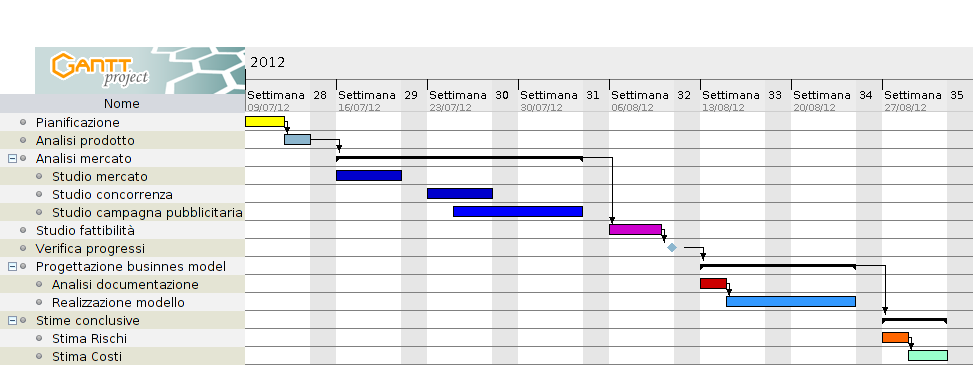
\includegraphics[scale=0.4]{images/cap3/Gantt.png}
\caption{Gannt}
\end{figure}

\vspace*{0.5cm}

Dato il grado non troppo elevato di questa fase dovuta ad una progettazione strutturata su molte figure diverse e specializzate, si è ritenuto opportuno lo sviluppo del progetto seguendo un ciclo di vita cosiddetto a cascata, che prevede quindi il susseguirsi delle varie fasi auto-conclusive, e che alla loro chiusura prevedono la documentazione necessaria e sufficiente per l'avanzamento alla fase successiva.

\subsection{Descrizione delle fasi}
\begin{itemize}

\item Analisi del prodotto: prima di affrontare lo studio di mercato, concorrenza e campagna pubblicitaria, i principali esperti del nostro team devono approfondire lo stato in essere del nostro prodotto.

\item Analisi di mercato: studio del mercato in cui si colloca il nostro prodotto.
\begin{itemize}

\item Studio di mercato: studio del mercato dell'ambito della sicurezza sul lavoro.

\item Studio della concorrenza: studio dei principali competitors e delle loro offerte.

\item Studio campagna pubblicitaria:a seguito dei dati raccolti studio un'efficace campagna pubblicitaria per il nostro prodotto.

\end{itemize}

\item Studio fattibilità: ha lo scopo di valutare tutti i dati raccolti nella fase di analisi di mercato per sancire se il nostro prodotto è commercializzabile e possa avere una possibilità di successo a fronte delle offerte dei competitors.

\item Verifica progressi: fase di verifica dell'avanzamento del lavoro, dove il capo progetto deve assicurarsi che i lavori siano giunti al punto prestabilito. Qui termina la fase di raccolta dati per dare inizio alla creazione del Business Model. 

\item Progettazione Business Model:

\begin{itemize}

\item Analisi documentazione: si analizzano i dati e le conclusioni ottenuti dalle fasi precedenti, condividendo le informazioni con tutti gli esperti del nostro team.

\item Realizzazione modello: fase di progettazione del business model.

\end{itemize}

\item Stima rischi: stima dei rischi riscontrabili dal nostro business model e delle possibili soluzioni ad essi.

\item Stima costi: stima dei costi necessari per supportare il business model scelto.

\end{itemize}


\subsection{Distribuzione delle risorse}
Alcuni compiti saranno svolti dal membro del gruppo che ricopre il ruolo corrispondente, ad esempio il compito \virgolette{Raccolta dati sicurezza} sarà svolto dal membro del gruppo che ricopre la figura di \virgolette{Esperto sicurezza}, altri saranno svolti da più membri contemporaneamente, come ad esempio \virgolette{Progettazione Business Model}, ma vediamo in dettaglio la distribuzione delle risorse del team rispetto le fasi operative: \\

\begin{figure}[H]
\centering
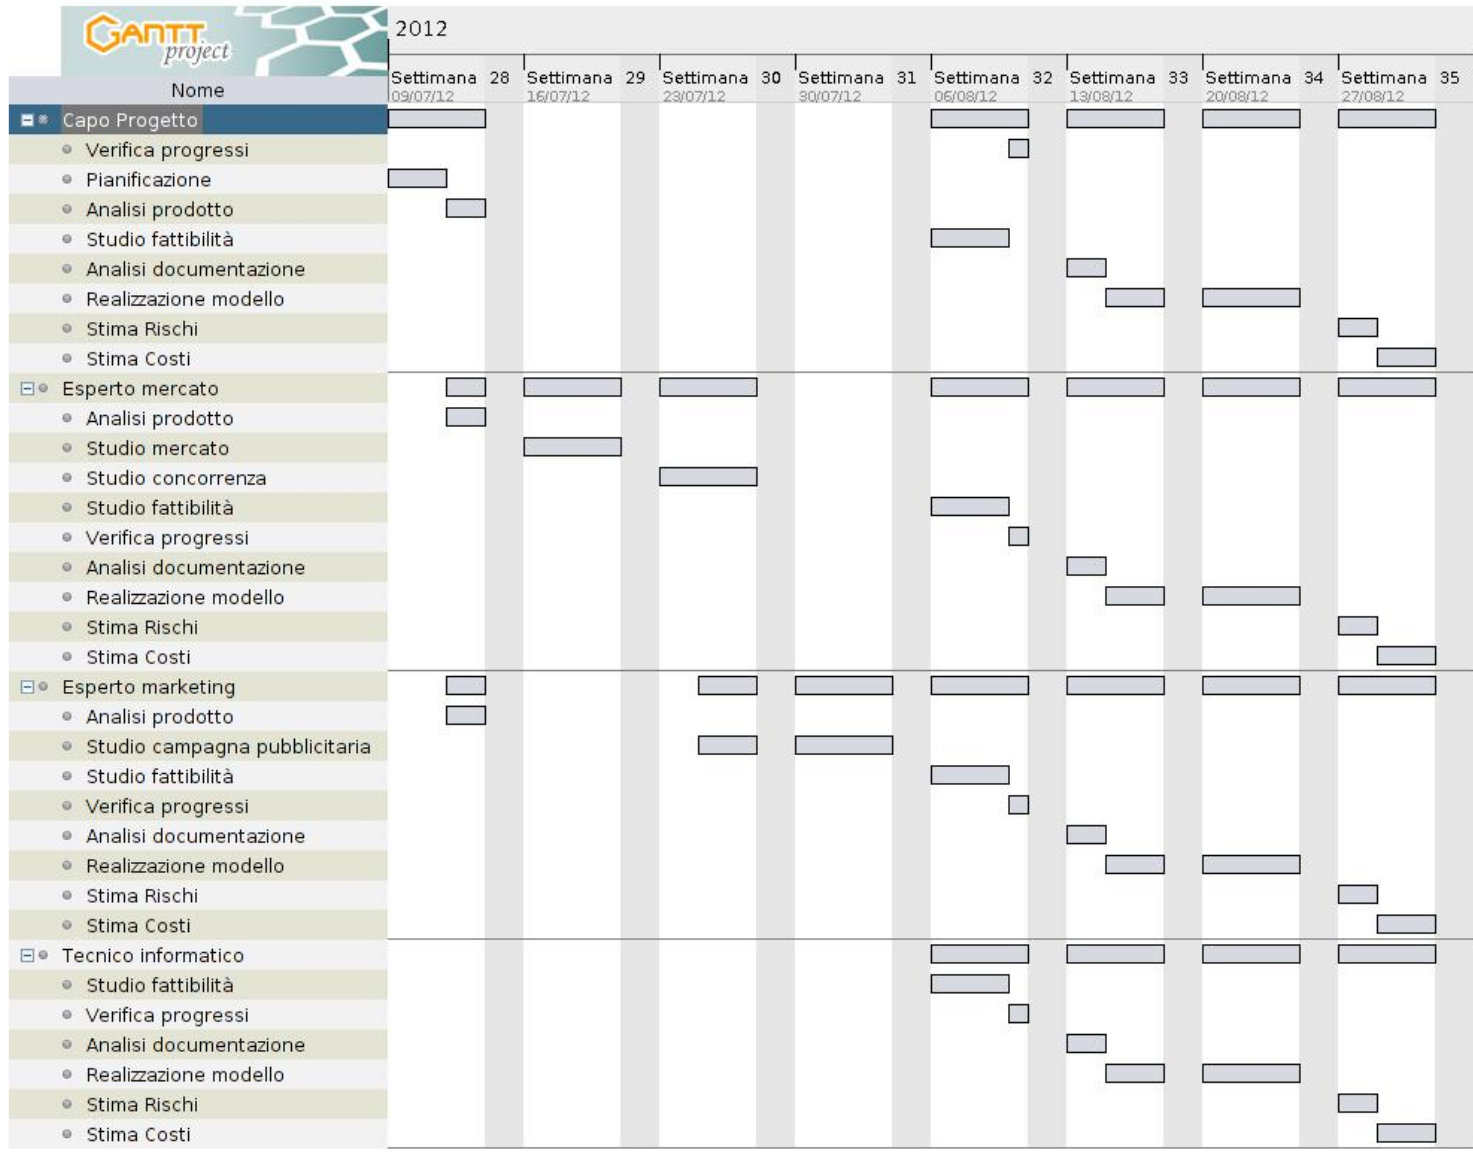
\includegraphics[scale=0.65]{images/cap3/risorse.png}
\caption{Distribuzione risorse}
\end{figure}

\vspace*{0.5cm}

Nella figura \virgolette{Distribuzione risorse} si può vedere come le varie figure partecipanti al lavoro siano impegnate temporalmente su tutto il periodo di attività.

\newpage
\subsection{Pianificazione oraria e dei costi}

In questa sezione sarà proposto il preventivo che risulta dalle ipotesi sulla quantità di ore che servirà ad ogni figura professionale per svolgere la propria parte di progetto.\\
Il preventivo sarà calcolato tramite i costi medi orari (CMO) riassunti nella seguente tabella:\\

\begin{longtable}{ | p{5cm} | p{3.4cm} |}
\caption{Compenso orario delle figure professionali}\\
\hline
\endfirsthead
\multicolumn{2}{r}{\textit{(Continua alla pagina successiva)}}
\endfoot
\multicolumn{2}{l}{\textit{(Continua dalla pagina precedente)}}
\endhead
\hline
\endlastfoot
\textbf{Figura professionale} \ & \textbf{CMO}\\
\hline
\rule[-2mm]{0mm}{0.7cm}
Capo progetto & \EUR \ 40 \\
\hline
\rule[-2mm]{0mm}{0.7cm}
Esperto mercato & \EUR \ 25 \\
\hline
\rule[-2mm]{0mm}{0.7cm}
Esperto marketing & \EUR \ 25 \\
\hline
\rule[-2mm]{0mm}{0.7cm}
Tecnico informatico & \EUR \ 30 \\
\hline
\end{longtable}


\begin{longtable}{ | p{5cm} | p{3.5cm} | p{3.5cm} |}
\caption{Preventivo costi totali per ogni figura professionale}\\
\hline
\endfirsthead
\multicolumn{3}{r}{\textit{(Continua alla pagina successiva)}}
\endfoot
\multicolumn{3}{l}{\textit{(Continua dalla pagina precedente)}}
\endhead
\hline
\endlastfoot
\textbf{Figura professionale} \ & \textbf{Ore preventivate} \ & \textbf{Costi preventivati} \\
\hline
\rule[-2mm]{0mm}{0.7cm}
Capo progetto & 100 (25 giorni) & \EUR \ 4.000\\
\hline
\rule[-2mm]{0mm}{0.7cm}
Esperto mercato & 128 (32 giorni)& \EUR \ 3.200 \\
\hline
\rule[-2mm]{0mm}{0.7cm}
Esperto marketing & 90 (30 giorni) & \EUR \ 2.250 \\
\hline
\rule[-2mm]{0mm}{0.7cm}
Tecnico informatico & 100 (20 giorni) & \EUR \ 3.000 \\
\hline
\rule[-2mm]{0mm}{0.7cm}
\textbf{Totale} & \textbf{408} (8 settimane) & \textbf{\EUR \ 12.450} \\
\hline
\end{longtable}

Viene inoltre proposta la tabella con i costi preventivati per ogni fase di progetto indicata nella pianificazione:

\begin{longtable}{ | p{6cm} | p{4cm} |}
\caption{Preventivo costi per fase di progetto}\\
\hline
\endfirsthead
\multicolumn{2}{r}{\textit{(Continua alla pagina successiva)}}
\endfoot
\multicolumn{2}{l}{\textit{(Continua dalla pagina precedente)}}
\endhead
\hline
\endlastfoot
\textbf{Fase di progetto} \ & \textbf{Costi preventivati}\\
\hline
\rule[-2mm]{0mm}{0.7cm}
Pianificazione e Analisi prodotto & \EUR \ 1.150 \\
\hline
\rule[-2mm]{0mm}{0.7cm}
Analisi di mercato & \EUR \ 1.600 \\
\hline
\rule[-2mm]{0mm}{0.7cm}
Studio di fattibilità & \EUR \ 1.940 \\
\hline
\rule[-2mm]{0mm}{0.7cm}
Verifica progressi & \EUR \ 485 \\
\hline
\rule[-2mm]{0mm}{0.7cm}
Progettazione business model & \EUR \ 4.850 \\
\hline
\rule[-2mm]{0mm}{0.7cm}
Stime conclusive & \EUR \ 2.425 \\
\hline
\rule[-2mm]{0mm}{0.7cm}
\textbf{Totale} & \textbf{\EUR \ 12.450} \\
\hline
\end{longtable}

Questi dati saranno poi confrontabili con il quantitativo orario svolto effettivamente e le spese sostenute nel consuntivo.




% --------------------------------------------------------------------

%####################################################
%   cap Lory
%####################################################

\chapter{Analisi di mercato}

\section{Introduzione}

L'analisi sugli infortuni che segue si riferisce a dati relativi solo all'ambito italiano in quanto prevediamo una diffusione iniziale del software solo a livello nazionale.\\
Per un possibile ampliamento di mercato fare riferimento al capitolo Business Model.



%\subsection{Infortuni sul lavoro: statistiche}

\section{Bilanci infortunistici 2011}
Di seguito verranno riportati alcuni valori sugli infortuni sul lavoro registrati nell'ultimo decennio e in particolare verranno analizzati più dettagliatamente i valori registrati nel 2011.

\subsection{Visione genarale}


Ammontano a circa 920 i morti sul lavoro registrati nel 2011, pari a più di due persone ogni giorno.\\
Questo dato è in lieve calo rispetto ai 973 morti registrati nel 2010, ma nonostante ciò la cifra rimane ancora poco rassicurante.\\
Secondo il rapporto annuale dell'Inail anche gli infortuni sul lavoro registrati hanno visto un lieve calo, passando dai 776mila del 2010 agli 725mila del 2011, registrando una flessione del 6,6\%, pari a 51mila casi in meno.\\

\begin{figure}[H]
\centering
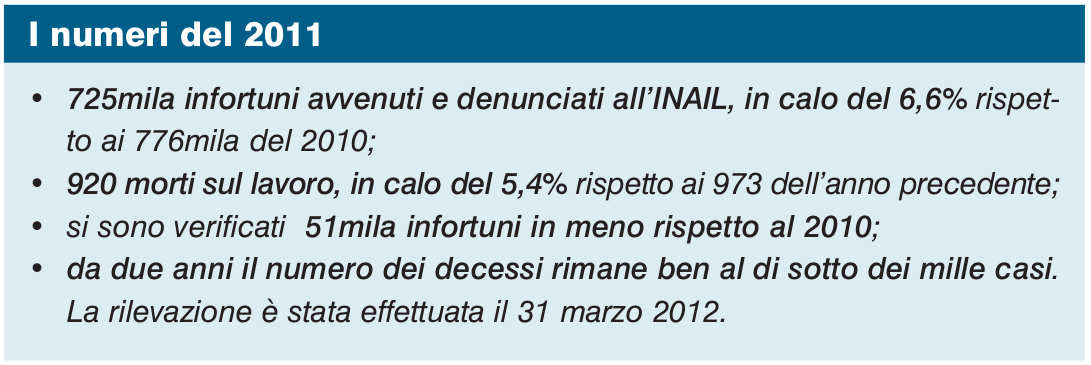
\includegraphics[scale=0.3]{images/cap4/analisiDiMercato/infortuniGenerale}
\caption{I numeri del 2011, fonti INAIL}
\end{figure}


In queste cifre non rientrano però gli infortuni relativi ai quasi 3 milioni (secondo i dati Istat) di lavoratori in nero presenti nel notro paese, tra i quali l’Istituto stima che nel 2010 (ultima proiezione disponibile) siano accaduti circa 164mila casi di infortunio.\\

\begin{figure}[H]
\centering
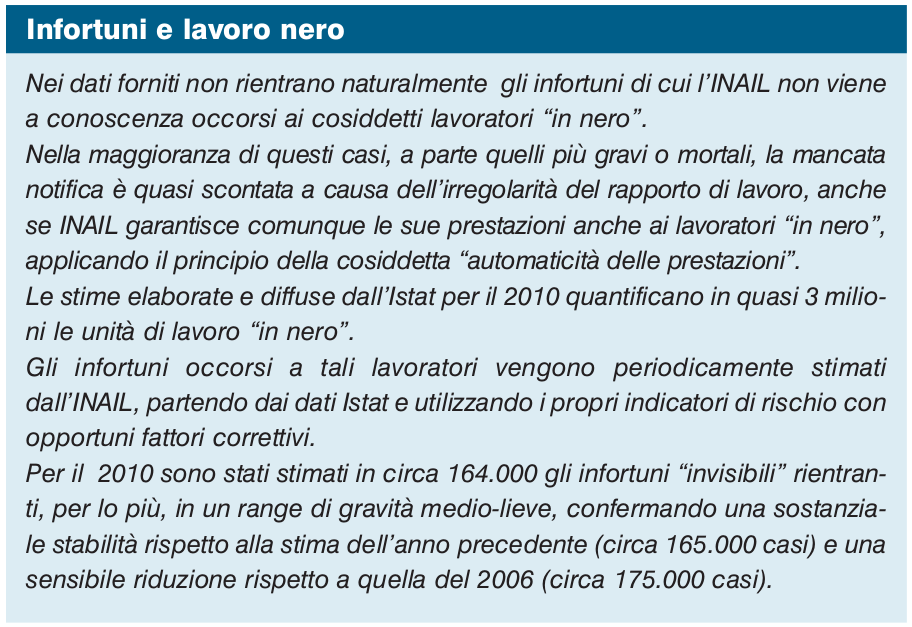
\includegraphics[scale=0.4]{images/cap4/analisiDiMercato/infortuniLavoroNero}
\caption{Infortuni e lavoro nero, fonti INAIL}
\end{figure}

Tra le 21.201 aziende controllate dall'Inail nel 2011, ben l’85,59\% è risultato ''irregolare'' per l’efficienza dei sistemi di scelta, della procedura cosiddetta di business intelligence che individua gli insiemi da controllare. Sono stati inoltre regolarizzati 48.716 lavoratori (nel 2010 erano stati 56.751), di cui 41.207 irregolari e 7.509 in nero (4.426 nel terziario, 2.675 nell’industria).\\\\



\
\
\
**business intelligence: un insieme di processi aziendali per raccogliere ed analizzare informazioni strategiche.\\\\

\ \
\subsection{Statistiche nel dettaglio}

\textbf{Infortuni per modalità di evento}\\
Per procedere in un’analisi dettagliata dei valori sugli infortuni sul lavoro, vanno prima di tutto distinte le modalità in cui avviene l’infortunio:

\begin{itemize}
\item \textbf{in occasione di lavoro} sono i casi che avvengono nell’esercizio effettivo dell’attività;
\item \textbf{in itinere} sono invece quelli che accadono al di fuori del luogo di lavoro, durante il per-
corso casa-lavoro-casa.
\end{itemize}


E' possibile notare una diminuzione tra il 2010 e il 2011 su entrambe le tipologie di infortuni:\\
negli infortuni in itinere si è registrata una flessione del 7,1\%, passando da 88.129 casi del 2010 a 81.861 nel 2011;\\
mentre negli infortuni avvenuti in occasione di lavoro, che rappresentano circa il 90\% del com-
plesso delle denunce, la flessione è stata invece pari a 6,5\%.\\
Da notare come ben il 90\% degli infotuni si concentri unicamente nei settori lavorativi riguardanti \textit{l'industria e i servizi}: questo dato può far riflettere molto sull'utilità di sviluppare una buona prevenzione sugli infortuni sul lavoro mirata soprattutto a quensti settori fortemente a rischio.\\
Il restante 10\% degli incidenti invece è ripartito per il 6\% nel settore \textit{agricolo} e per il 4\% tra i \textit{dipendenti del conto Stato}.


\begin{figure}[H]
\centering
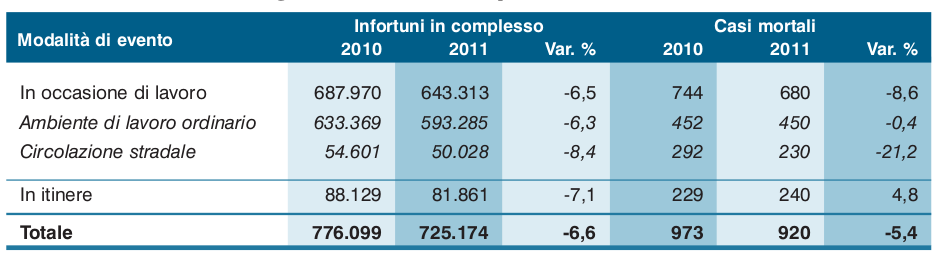
\includegraphics[scale=0.5]{images/cap4/analisiDiMercato/infortuniPerModalita}
\caption{Infortuni denunciati 2010-2011, per modalità di evento}
\end{figure}


\textbf{Infortuni per attività}\\
Dall’analisi settoriale si può notare come nel 2011 la diminuzione degli infortuni sul lavoro, rispet-
to all’anno precedente, abbia interessato in primo luogo il settore dell’Industria (-8,2\%), dell’Agricoltura (-6,5\%) e le attività dei Servizi (-5,5\%), che sono i tre settori con il maggior numero di infortuni.
Durante lo stesso periodo va segnalata però, secondo i dati Istat, una diminuzione degli occupati nell’Industria dello 0,6\% e nell’Agricoltura dell’1,9\% e, viceversa, una leggera ripresa nei Servizi (+1\%).
Tra le attività nel dettaglio, si distinguono per una elevata riduzione degli infortuni le
Costruzioni (-14,7\%) a fronte di un calo occupazionale del 5,3\%, seguite con un più con-
tenuto ma significativo calo da importanti settori quali la Meccanica (-6,7\%) e la
Metallurgia (-6,6\%).
Nei Servizi la diminuzione degli infortuni è ha riguardato in maggior modo i settori
più rilevanti dal punto di vista dimensionale: Trasporti (-11,3\%), Servizi alle imprese e atti-
vità immobiliari (-9,7\%), Commercio (-9,6\%). Anche per il settore del personale addetto
ai servizi domestici si segnala un calo contenuto del 3,4\%.
Per quanto riguarda i casi mortali, analizzando le attività nel dettaglio, si è registrato nel
2011 una diminuzione sensibile dei Servizi (-9,4\%) e dell’Industria (-3,7\%), mentre per
l’Agricoltura si segnala un +2,7\%. Tra i settori più rilevanti, una riduzione molto elevata
si è verificata nei Trasporti (-30,7\%), nei Servizi alle imprese e attività immobiliari (-26,2\%)
e le Costruzioni (-10,6\%). Viceversa, sono aumentate le vittime nell'ambito dell’ Industria pesante della Metalmeccanica.\\\\


\begin{figure}[H]
\centering
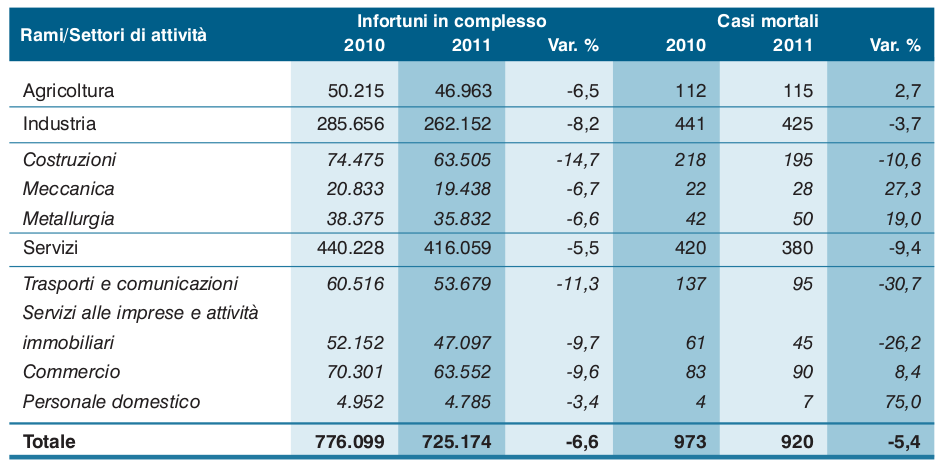
\includegraphics[scale=0.5]{images/cap4/analisiDiMercato/infortuniPerGestione2}
\caption{Infortuni denunciati 2010-2011, per settori e attività}
\end{figure}








\textbf{Infortuni per sesso}\\
Nel 2011 il calo infortunistico ha interessato sia i lavoratori (-7,0\%) che le
lavoratrici (-5,6\%).\\
Per quanto riguarda invece il calo complessivo degli infortuni mortali  (-5,4\%), questa flessione è influenzata esclusivamente dei lavoratori di sesso maschile, poichè al contrario, gli infortuni mortali sul lavoro del sesso femminile, hanno riscontrato un sensibile aumento dei decessi (+15,4\%, passando dai 78 casi del 2010 ai 90 del 2011). Tale aumento è dovuto prevalentemente ai casi in itinere che rappresentano più della metà dei decessi femminili.
Per questi valori, va considerato che, secondo i dati Istat, le donne rappresentano circa il 40\% degli
occupati, e che la quota di infortuni femminili rispetto al totale è del 32\% e quasi il 10\% per
i casi mortali. Da questo \textit{si deduce che il lavoro femminile è sicuramente meno rischioso}; le donne
sono, infatti, occupate prevalentemente nei servizi e in settori a bassa pericolosità e, se
impegnate in comparti più rischiosi come quello delle Costruzioni, dei Trasporti e
dell’Industria pesante, svolgono comunque mansioni di tipo impiegatizio o dirigenziale.


\begin{figure}[H]
\centering
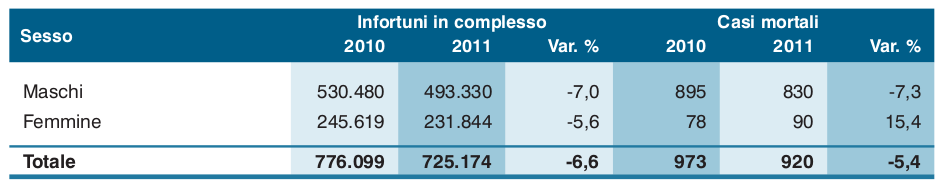
\includegraphics[scale=0.5]{images/cap4/analisiDiMercato/infortuniPerSesso1}
\caption{Infortuni denunciati 2010-2011, per sesso}
\end{figure}

\begin{figure}[H]
\centering
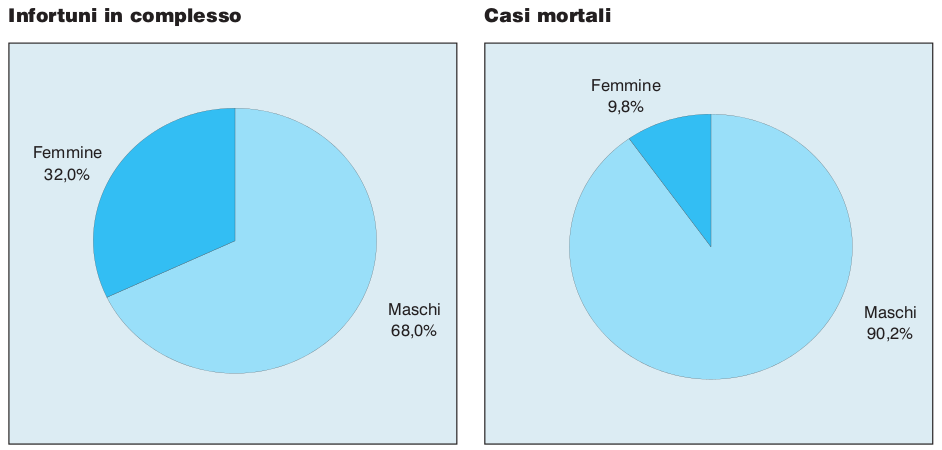
\includegraphics[scale=0.5]{images/cap4/analisiDiMercato/infortuniPerSesso2}
\caption{Infortuni per sesso, anno 2011}
\end{figure}

\textbf{Infortuni per età}\\
Analizzando i dati per fascia di età, è facile notare che la fascia tra i 35-49 risulta la più colpita con ben il 44\% di tutti gli infortuni, mentre la seconda fascia di età più colpita risulta essere quella fino ai 34 anni, con il 32\% degli infortuni complessivi.

\begin{figure}[H]
\centering
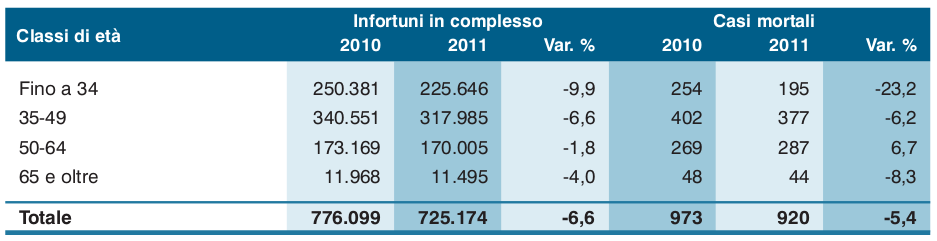
\includegraphics[scale=0.5]{images/cap4/analisiDiMercato/infortuniPerEta1}
\caption{Infortuni denunciati 2010-2011, per età}
\end{figure}

\begin{figure}[H]
\centering
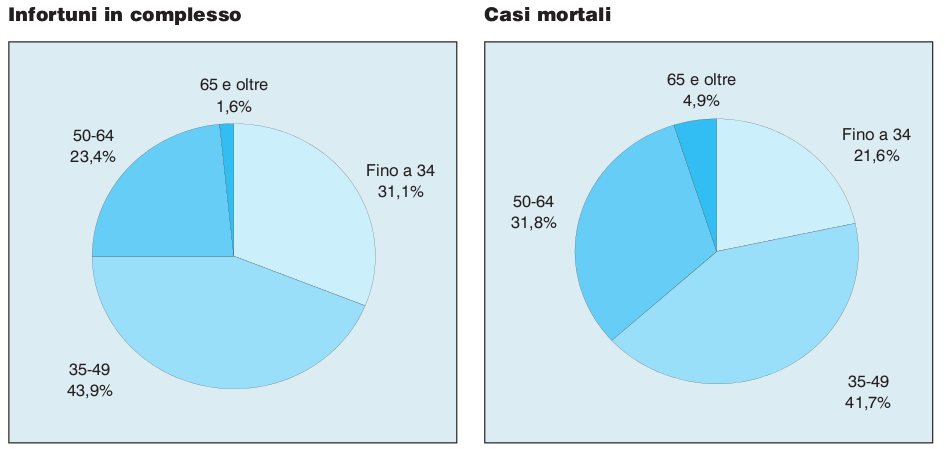
\includegraphics[scale=0.53]{images/cap4/analisiDiMercato/infortuniPerEta2}
\caption{Infortuni per età, anno 2011}
\end{figure}







\ \ \
\section{Bilanci infortunistici ultimo decennio 2002-2011}
\ \
\subsection{Visione genarale}

Ampliando l'osservazione dei dati sugli infortuni sul lavoro all'ultimo decennio, si può notare come il calo registrato nel 2011, rientri in un andamento decrescente delle denunce di infortunio:
\begin{itemize}
\item tra il 2002 e il 2011 le denunce sono scese da 992.665 a 725.174;
\item la contrazione complessiva è stata del 26,9\% (circa 268.000 infortuni in meno).
\end{itemize}



\ \
\subsection{Statistiche nel dettaglio}

\textbf{Infortuni per attività}\\
Scomponendo il fenomeno secondo i tre grandi rami di attività previsti dalla classifica-
zione Istat, si registra, dal 2002 al 2011, una diminuzione degli infortuni sul lavoro sensibile e costante in Agricoltura (pari a -36,1\%) e nell’Industria (-44,0\%). Anche nei
Servizi, dopo anni di sostanziale stabilità, la riduzione è divenuta apprezzabile (-7,8\%).



\begin{figure}[H]
\centering
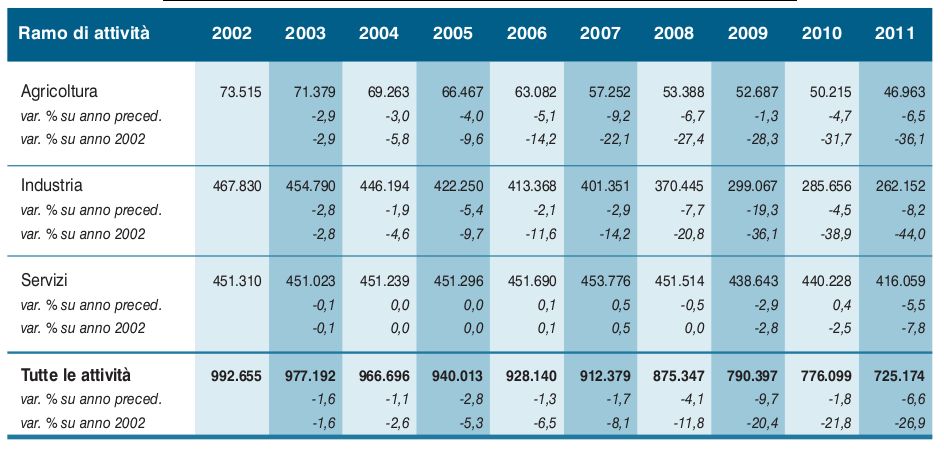
\includegraphics[scale=0.5]{images/cap4/analisiDiMercato/infortuniDecennioPerGestione1}
%\caption{Infortuni per attività, decennio 2002-2011}
\end{figure}

\begin{figure}[H]
\centering
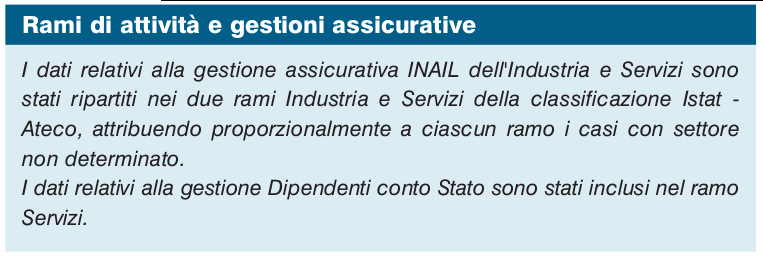
\includegraphics[scale=0.55]{images/cap4/analisiDiMercato/infortuniDecennioPerGestione2}
\caption{Infortuni per attività, decennio 2002-2011}
\end{figure}



\textbf{Infortuni per modalità}\\
La flessione ha riguardato esclusivamente gli infortuni in occasione di lavoro ( cioè durante il reale
ambito lavorativo):\\
tra il 2002 (920.299 denunce) e il 2011 (643.313 denunce) gli infortuni in occasione di
lavoro hanno fatto registrare un consistente calo di oltre il 30\%.\\

Nello stesso periodo, invece, gli infortuni in itinere sono passati dai 72.356 casi denunciati del 2002 agli 81.861 del 2011 con una crescita del 13,1\%, anche se già a partire dal
2009 (92.926 casi) si assiste ad un calo dei casi, dopo anni di costante aumento.
La quota di infortuni in itinere sul totale degli infortuni è aumentata nel decennio, dal
7,3\% del 2002 all’11,3\% del 2011.


\begin{figure}[H]
\centering
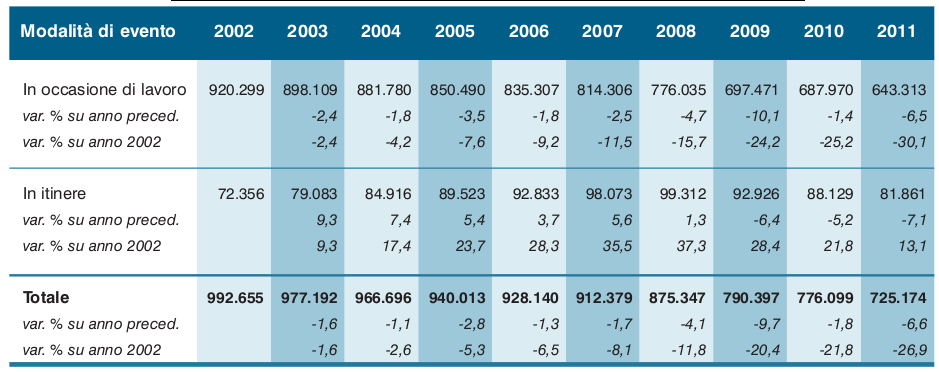
\includegraphics[scale=0.55]{images/cap4/analisiDiMercato/infortuniDecennioPerModalita}
\caption{Infortuni per modalità, decennio 2002-2011}
\end{figure}




Nel periodo 2002-2011, a livello di singolo ramo di attività è possibile notare le seguenti variazioni significative:
\begin{itemize}
\item l’Industria detiene ancora il risultato migliore, con una contrazione complessiva dell’indice di incidenza del 42,6\% (calo degli occupati registrato dall’Istat del 2,4\%);
\item l’Agricoltura segue con -25,6\% (calo degli occupati del 14,1\%);
\item inferiore il calo del ramo Servizi (-15,8\%), che è il solo comunque a beneficiare di
un positivo andamento nelle dinamiche occupazionali (crescita del 9,5\%).\\
\end{itemize}


\textbf{Infortuni mortali}\\
Anche per quanto riguarda gli infortuni mortali, nel periodo 2002-2011 si conferma una costante decrescita e le serie storiche rivelano gli enormi progressi compiuti dai primi anni sessanta, quando si toccò nel 1963, in pieno boom economico il tragico record storico di 4.664 morti in un solo anno.
Più in dettaglio, il calo dei morti sul lavoro, registrato nel decennio di interesse, risulta molto
sostenuto in tutti e tre i grandi rami di attività:
\begin{itemize}
\item Agricoltura -31,1\%,
\item Industria -41,3\%,
\item Servizi -35,3\%).\\
\end{itemize}

Le difformità tra i rami sono da attribuire, alla diversa dinamica occupazionale che ha registrato nel periodo osservato, un calo del 14,1\% in Agricoltura, un calo più modesto nell’Industria (-2,4\%) e una crescita del 9,5\% nei Servizi.



\begin{figure}[H]
\centering
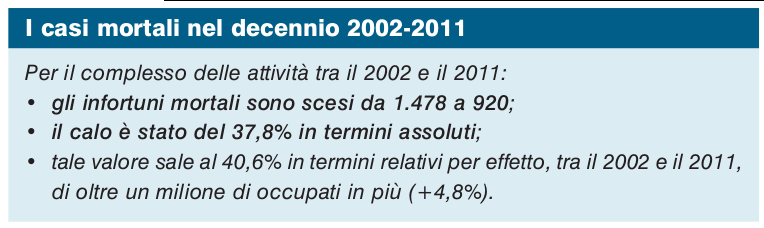
\includegraphics[scale=0.5]{images/cap4/analisiDiMercato/infortuniDecennioPerMortalita1}
\caption{Infortuni per mortalità, decennio 2002-2011}
\end{figure}

\begin{figure}[H]
\centering
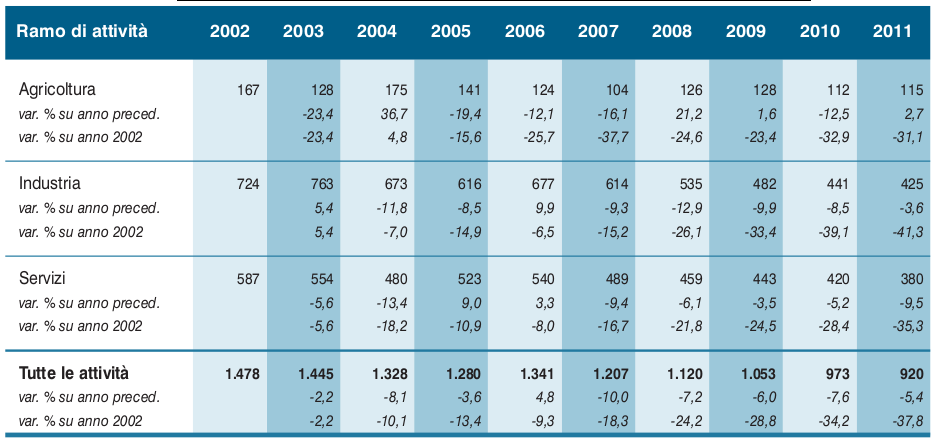
\includegraphics[scale=0.55]{images/cap4/analisiDiMercato/infortuniDecennioPerMortalita2}
\caption{Infortuni per mortalità riassunto, decennio 2002-2011}
\end{figure}





\textbf{Infortuni mortali per modalità}\\
Per gli eventi mortali è importante disinguere tra i decessi avvenuti nello
svolgimento della propria mansione lavorativa (in occasione di lavoro) e quelli in itinere
(gli infortuni avvenuti in genere nel percorso di spostamento casa-lavoro-casa).
La distinzione è importante poichè si può ragionevolmente ritenere che i decessi in
itinere non siano strettamente collegati alla specifica attività svolta dall’infortunato e quin-
di richiedano anche una diversa valutazione nella lettura del rischio che determina il
fenomeno infortunistico.



\begin{figure}[H]
\centering
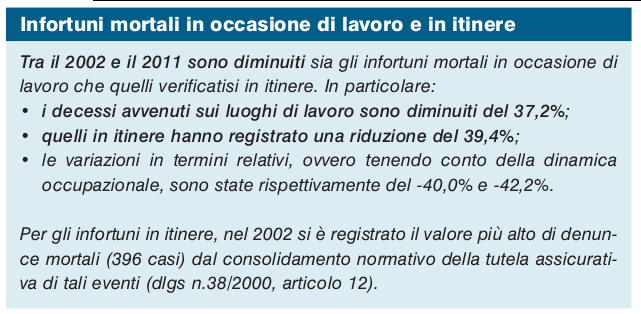
\includegraphics[scale=0.55]{images/cap4/analisiDiMercato/infortuniDecennioMortaliPerModalita1}
\caption{Infortuni mortali per modalità riassunto, decennio 2002-2011}
\end{figure}

\begin{figure}[H]
\centering
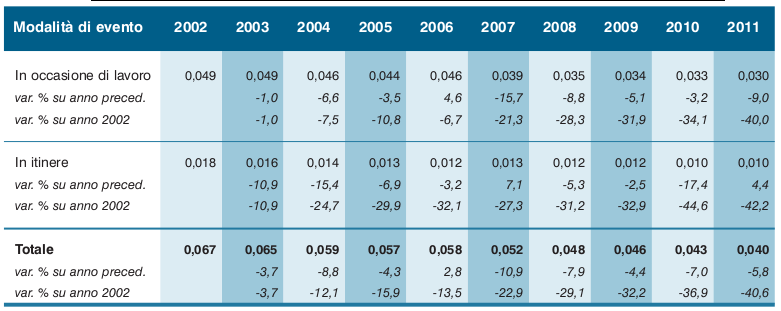
\includegraphics[scale=0.65]{images/cap4/analisiDiMercato/infortuniDecennioMortaliPerModalita2}
\caption{Infortuni mortali per modalità, decennio 2002-2011}
\end{figure}



\textbf{Infortuni per nazionalità}\\
Dagli ultimo dati Istat, è emerso che gli stranieri residenti in Italia al 1° gennaio 2011 sono
4.570.317, 335 mila in più rispetto all’anno precedente (+7,9\%).\\
Questi cittadini rappresentano un valore molto influente sui dati sugli infortuni sul lavoro, considerando che nel 2011 i lavoratori stranieri assicurati all’INAIL sono stati circa 3 milioni, valore che ha visto un incremento dell’1,3\% in più rispetto all'anno precedente e del 17,8\% in più del 2007.\\


\begin{figure}[H]
\centering
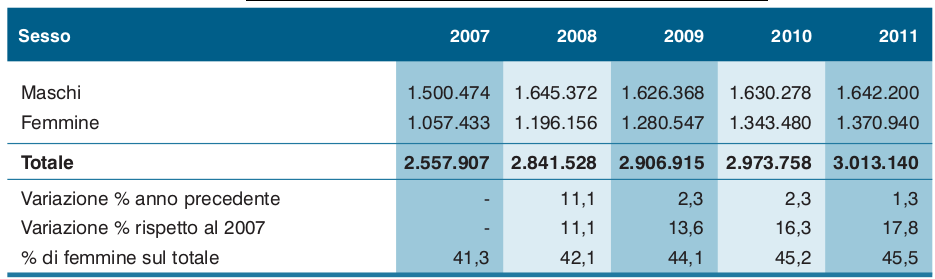
\includegraphics[scale=0.55]{images/cap4/analisiDiMercato/lavoratoriStranieri1}
\caption{Lavoratori stranieri assicurati all’INAIL per sesso}
\end{figure}

\begin{figure}[H]
\centering
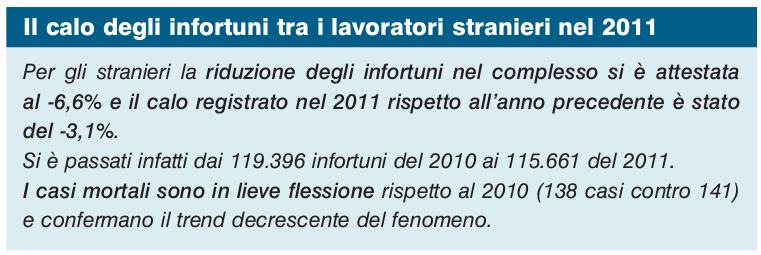
\includegraphics[scale=0.55]{images/cap4/analisiDiMercato/lavoratoriStranieri2}
\caption{Infortuni nei lavoratori stranieri}
\end{figure}



Gli infortuni degli stranieri rappresentano il 15,9\% degli infortuni complessivi, quelli dei
soli extracomunitari, invece, l’11,7\%; se si considerano i casi mortali le percentuali sono
rispettivamente del 15\% e dell’ 8,8\%.\\
In generale risulta che il 94,3\% degli infortuni degli stranieri si verifica nell’Industria e
servizi, il 5\% in Agricoltura e lo 0,7\% tra i Dipendenti conto Stato.\\
Da questi dati possiamo ricavare che non deve essere sottovalutata la fascia di lavoratori stranieri presente nel nostro paese in quanto rappresenta una percentuale non esigua e lo stesso va affermato per il numero di infortuni occorsi.\\



\textbf{Infortuni e indennizzi}\\
Gli infortuni indennizzati ogni anno dall'Inail sono circa 500.000 ogni anno, con una flessione che va da 650.000 nell'anno 2007, ai 478.000 nel 2011.\\
E' pertanto ipotizzabile che le somme di denaro spese dall'Inail per gli indennizzi sugli infortuni sul lavoro siano ingenti.\\
Di seguito viene riportato un rapporto sul numero degli infrotuni indennizzati nell'ultimo quinquennio:

\begin{figure}[H]
\centering
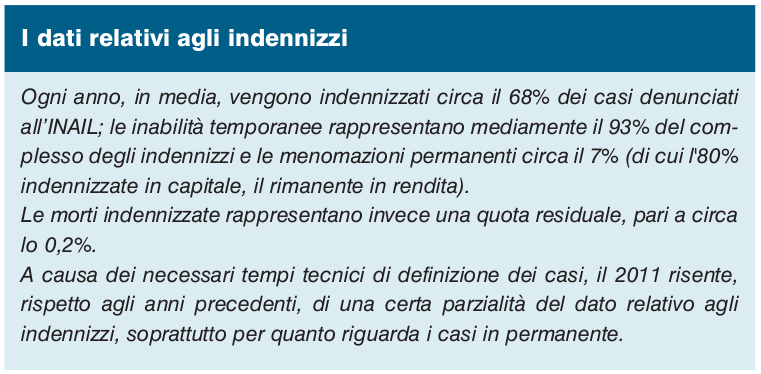
\includegraphics[scale=0.55]{images/cap4/analisiDiMercato/infortuniIndennizzi1}
\caption{Infortuni e indennizzi}
\end{figure}

\begin{figure}[H]
\centering
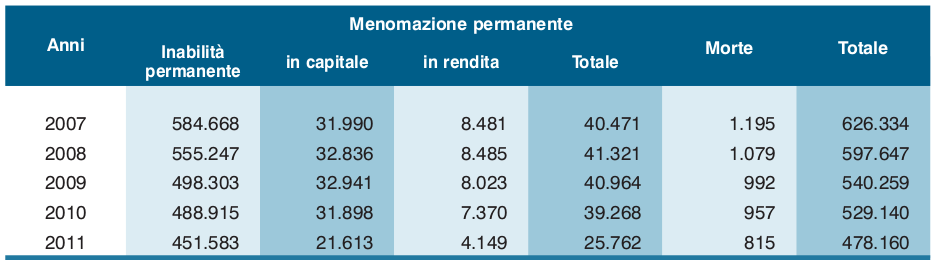
\includegraphics[scale=0.55]{images/cap4/analisiDiMercato/infortuniIndennizzi2}
\caption{Infortuni indennizzati nel quinquennio 2007-2011 per tutte le gestioni}
\end{figure}




\ \ \
\section{Osservazioni sui bilanci}
Dai bilanci Inail sugli infortuni sul lavoro riportati nelle sezioni precedenti, è possibile effettuare un'attenta lettura nel dettaglio, così da ricavare delle importanti osservazioni utili per capire come meglio sviluppare e incentrare il progetto Woty.\\
In primo luogo infatti è possibile comprendere quali siano i settori lavorativi più a rischio infortuni sul lavoro, nei quali il software Woty potrebbe avere una maggiore e più facile diffusione; e in secondo luogo è possibile comprendere quali siano le fasce di popolazione più a rischio infortuni, distinte per età, sesso e nazionalità.\\
E' molto importante infatti adempiere ad uno sviluppo \virgolette{mirato}, in particolar modo nella prima fase di sviluppo e di distribuzione del software, così da poter minimizarre i fattori di rischio iniziali.\\


\subsection{Woty: quali settori e attività lavorativi?}
Dai dati Inail relativi agli infortuni sul lavoro nell'ultimo decennio, si evince che la graduatoria dei settori lavorativi per il maggior numero di infortuni, vede al primo posto il settore dei \textbf{Servizi} che dal 2002 registra ogni anno più di 400.000 casi ( 450.000 casi nel 2002 - 416.000 casi nel 2011).\\
Al secondo posto troviamo il settore dell' \textbf{Industria} che registra una media di 350.000 casi nell'ultimo decennio. Gli infortuni in questo settore sono però in costante dimunizione e sono passati dai 460.000 casi nel 2002 ai 260.000 casi nel 2011.\\
Al terzo posto si classifica il settore dell' \textbf{Agricoltura} con una media di 50.000 casi all'anno. Anche in questo settore il numero è in lieve ma continua diminuzione registrando una variazione di circa 20.000 casi nell'ultimo decennio: 73.000 casi nel 2002 e 46.000 casi nel 2011.\\

Da ciò è possibile ricavare come i settori più indirizzati per lo sviluppo e diffusione di Woty sono i settori dei Servizi e dell'Industria, in quanto in questi due settori avviene il 90\% dei casi di infortuni.\\
Più nel dettaglio, osservando i dati Inail sugli infortuni per singola attività registrati nel 2011, nel settore dei servizi ad avere i valori più alti di infortuni sono le attività del \textbf{commercio} e dei \textbf{trasporti e comunicazioni}, mentre nel settore dell'industria le attività con i maggiori valori di infortuni sono quelle delle \textbf{costruzioni} e della \textbf{metallurgia}.\\
Ne consegue che saranno queste le attività lavorative verso le quali Woty dovrà indirizzarsi per poter avere una maggiore e più facile diffusione del software limitando i rischi di fallimento.\\


Tra le attività individuate come più adatte per l'utilizzo del software Woty, possiamo evidenziare come al loro interno siano presenti sia lavoratori con postazione fissa, sia lavoratori in mobilità; pertanto la piattaforma Woty potrà essere sfruttata nella sua interezza risultando così idonea agli ambiti di applicazione:\\
- per i lavoratori che dispongono di postazione fissa potrà essere utilizzato l'applicativo Woty desktop raggiungibile tramite dispositivi pc o notebook utilizzando un normale browser di navigazione internet\\
- per i lavoratori in mobilità presenti in ampia misura per esempio nei settori dei trasporti e del commercio, potrà essere utilizzato l'applicativo Woty mobile, che attraverso l'app permette l'utilizzo della piattaforma Woty direttamente da dispositivi mobili.



\subsection{Woty: quali età nei lavoratori?}
Osservando i dati relativi agli infortuni sul lavoro 2011, in relazione alle età dei lavoratori interessati, è possibile notare come ad essere più colpiti siano gli occupati con età comprese tra i 35 e 49 anni con ben 340.000 casi registrati nell'anno 2011.
Al secondo posto troviamo invece gli occupati con età inferionre ai 34 anni con ben 250.000 casi registrati nell'anno 2011.\\
Questi dati risultano essere favorevoli per la diffusione e un buon utilizzo del sistema Woty, in quanto essendo questa piattaforma molto innovativa e tecnologica, è più facilmente utilizzabile da parte di lavoratori appartenenti alla fascia d'età più giovane.\\
E' facilmente intuibile infatti che un occupato di età giovanile sia più indicato all'utilizzo delle tecnologie innovative, quali l'uso costante del pc oppure l'uso di cellulari smartphone con applicazioni innovative.



\subsection{Woty: lavoratori stranieri?}
Dai valori Inail sulla percentuale di lavoratori stranieri nel 2011, è emerso che ammontano a circa 3 milioni i lavoratori di nazionalità straniera presenti nel nostro, e sempre nel 2011 si sono registrati circa 115.000 casi di infortuni sul lavoro da parte di questi lavoratori, cioè il 15\% degli infortuni complessivi.\\
I valori risultano essere sufficientemente alti da far si che questa fascia di lavoratori debba essere presa in considerazione in ambito di sviluppo e diffusione della piattaforma Woty.\\
Deve essere presa in considerazione quindi l'utilizzo di Woty anche da parte di lavoratori stranieri e quindi il software dovrà supportare degli adeguati multilingua per permetterne un utilizzo più esteso, questo in previsione anche di una diffusione del software su scala internazionale.





\url{http://www.inail.it/Portale/appmanager/portale/desktop?_nfpb=true&_pageLabel=PAGE_SALASTAMPA&nextPage=Prodotti/Dossier_e_Speciali/SPECIALE_RAPPORTO_ANNUALE_2011/index.jsp}

















%--------------------------- CONCORRENZA
%####################################################
%   cap Umba
%####################################################


\chapter{Concorrenza}

\section{Legislazione Vigente}

Con il decreto legislativo d.lgs. 626/94 si è andato ad approfondire quello che è l'ambito della sicurezza aziendale, introducendo tutta una nuova serie di obblighi per datori di lavoro e dipendenti. Tra questi obblighi possiamo trovare la necessità di formare tutti i collaboratori dell'azienda sui principali fattori di rischio, sulla prevenzione e sul primo soccorso, fino ad arrivare a nozioni più specialistiche riguardanti il tipo di azienda cui si appartiene e secondo la mansione che si ricopre.\\
Questa cosiddetta \virgolette{legge 626} è stata ora sostituita con il D.lgs. 81/2008 o \textit{Testo unico} sulla sicurezza sul lavoro ampliando notevolmente il carico di obblighi riguardanti l'informazione sulla sicurezza e la preparazione in suddetto ambito.\\
Per adeguare la propria azienda a questi standard ed essere in regola è necessario far seguire ai propri dipendenti dei corsi specifici. Questi corsi, se certificati, possono essere seguiti online, tenuti da terze parti o organizzati in azienda da personale addetto.\\
Woty intende quindi prendere parte all'ambito didattico per la sicurezza sostituendosi a uno di questi corsi.


\section{Concorrenza}

La formazione nel campo della sicurezza è trattata da una moltitudine di enti, associazioni, società private sia in ambito nazionale, sia in quello europeo. Certi di questi corsi sono gratuiti e questo può complicare la
commercializzazione del nostro prodotto.\\

Alcuni dei criteri presi in considerazione per valutare i corsi sono:

\begin{itemize}
	\item \textbf{Ambito} (nazionale, europeo)
	\item \textbf{Costo} (gratuito, a pagamento, prezzo per dipendente, etc.)
	\item \textbf{Locazione} (in sede, sede esterna, online, dispositivo mobile, etc.)
	\item \textbf{Localizzazione} (inglese, italiano, etc.)
	\item \textbf{Durata/Distribuzione oraria}
	\item \textbf{Utilizzo di Gamification} (peculiarità del nostro software)
\end{itemize}

Analizziamo quindi quali possono essere le principali minacce alla commercializzazione del nostro prodotto:


\begin{itemize}
	\item European Agency for Safety and Health at Work (EU-OSHA) (\url{http://osha.europa.eu})
		\begin{itemize}
			\item \url{http://www.healthy-workplaces.eu/it/hw2012}
			\item \url{http://www.healthy-workplaces.eu/it/media/ipad-app}
			\item \url{http://www.oiraproject.eu/}
		\end{itemize}
	\item INAIL (\url{http://www.ispesl.it/ew/ec2012/})
	\item PMI Servizi (\url{http://www.pmiservizi.it/corsi})
		\begin{itemize}
			\item Quotidiano Sicurezza (\url{http://itunes.apple.com/it/app/quotidiano-sicurezza/id419112770?mt=8})
		\end{itemize}
	\item ANFOS (Associazione Nazionale Formatori della Sicurezza sul Lavoro) (\url{http://www.anfos.it})
\end{itemize}

Vediamole ora nel dettaglio.

\section*{European Agency for Safety and Health at Work (EU-OSHA)}

L'agenzia europea per la salute e la sicurezza sul lavoro è la principale autorità in ambito europeo ed è una prolifica fonte di iniziative e progetti.\\
Gran parte delle risorse di quest'organizzazione è dedicata alla raccolta dati e alla pianificazione di convegni, attività che non minacciano la commercializzazione del nostro prodotto. Tuttavia l'organizzazione sfrutta una serie di partner localizzati nei principali paesi europei per l'organizzazione di corsi (fare riferimento a INAIL per l'analisi di questo punto) e inoltre sviluppa una serie di progetti, tra cui delle applicazioni online o per dispositivi mobile che potrebbero avere delle ripercussioni sul nostro prodotto. Analizziamole:

\begin{itemize}
	\item \textbf{Lavorare insieme per la prevenzione dei rischi} (\url{http://www.healthy-workplaces.eu/it/hw2012}) è una campagna che tratta nozioni di sicurezza e si presta anche come autovalutazione per aziende e dipendenti sulle sue principali tematiche. Questo sito online gratuito e localizzato in italiano non costituisce alcuna minaccia poiché fornisce solamente nozioni, ma non è regolamentato e non fornisce nessuna certificazione. Non può quindi sostituire un corso certificato.
	
	\item \textbf{Lavoriamo insieme – Campagna Ambienti di lavoro sani e sicuri} (\url{http://www.healthy-workplaces.eu/it/media/ipad-app}) è una delle pochissime applicazioni per dispositivi mobile che tratta l'argomento della sicurezza. Applicazione realizzata a seguito della campagna precedente. Non costituisce una minaccia poiché non permette la certificazione del dipendente.

	\item \textbf{Online Interactive Risk Assessment project} (\url{http://www.oiraproject.eu/}) web application in ambito della
sicurezza. Volge principalmente l'attenzione all'autovalutazione del proprio ambiente di lavoro e non offre certificazioni, quindi non rappresenta una minaccia.

\end{itemize}

\section*{INAIL}

Istituto Nazionale Assicurazione contro gli Infortuni sul Lavoro è il portavoce con sede nazionale delle principali iniziative organizzate dall'EU-OSHA. Oltre a campagne e seminari come \virgolette{Lavoriamo insieme per la prevenzione dei rischi}, che non intaccano il nostro mercato, l'INAIL organizza anche corsi e/o altre iniziative sulla sicurezza che portano a certificazione i partecipanti. Pur sembrando quindi una minaccia, classificheremo l'INAIL come opportunità poiché offre la possibilità di segnalare iniziative sulla sicurezza degne di nota di cui quest'ente si farà poi portavoce, fungendo da nostro partner/ente pubblicitario anziché competitor.

\section*{PMI Servizi}

Società di servizi per le piccole e medie imprese che si occupa di corsi di formazione per il personale aziendale.\\
Offre una varia gamma di corsi proprietari gratuiti online e offre la possibilità di ottenere un attestato a norma di legge il quale però è a pagamento. Essendo un servizio italiano online, il corso è in lingua italiana e frequentabile gratuitamente a qualsiasi orario da chiunque in possesso di un computer o di un dispositivo mobile.\\
Per gli esami il PMI Servizi è affiliato ad ANFOS e si rifà al suo listino prezzi.\\
Questa società offre inoltre \virgolette{Quotidiano Sicurezza} una notevole app per dispositivi mobile che offre nozioni, notizie, video guide, etc. sulla sicurezza nel lavoro. Nonostante non sia una minaccia per la nostra applicazione, quest'app deve essere monitorata. In caso gli sviluppatori aggiungano nuove funzionalità (ad esempio la possibilità di ottenere certificazioni a norma di legge tramite esami online) potrebbe divenire una potenziale minaccia.

\section*{Associazione Nazionale Formatori della Sicurezza sul Lavoro (ANFOS)}

Principale società italiana dedicata alla sicurezza sul lavoro. Offre una vasta gamma di servizi che spaziano dai corsi in aula a quelli online. Offre inoltre la possibilità di certificare i lavoratori a norma di legge.\\
Con questi servizi e oltre 560 sedi sul territorio l'ANFOS rappresenta il nostro maggior competitor.\\

Analizziamo ora le sue offerte per singolo individuo:

\begin{longtable}{ | l | r |}
\caption{Offerte ANFOS}\\
\hline
\endfirsthead
\multicolumn{2}{r}{\textit{(Continua alla pagina successiva)}}
\endfoot
\multicolumn{2}{l}{\textit{(Continua dalla pagina precedente)}}
\endhead
\hline
\endlastfoot
\textbf{Corso} \ & \textbf{Prezzo}\\
\hline
\rule[-2mm]{0mm}{0.7cm}
Corso formazione datore di lavoro quale R.S.P.P. modulo 1 e 2 & 80,00\EUR + Iva \\
\hline
\rule[-2mm]{0mm}{0.7cm}
Corso formazione Antincendio & 110,00\EUR + Iva \\
\hline
\rule[-2mm]{0mm}{0.7cm}
Corso per addetti al servizio aziendale di primo soccorso e gestione delle emergenze & 130,00\EUR + Iva \\
\hline
\rule[-2mm]{0mm}{0.7cm}
Corso aggiornamento addetto al servizio di primo soccorso & 70,00\EUR + Iva \\
\hline
\rule[-2mm]{0mm}{0.7cm}
Corso RLS & 200,00\EUR + Iva \\
\hline
\rule[-2mm]{0mm}{0.7cm}
Corso di formazione generale ed informazione lavoratore & 35,00\EUR + Iva \\
\hline
\rule[-2mm]{0mm}{0.7cm}
Corso formazione Carrellisti (Mulettisti) & 85,00\EUR + Iva \\
\hline
\rule[-2mm]{0mm}{0.7cm}
Corso di formazione per ricoprire il ruolo di Preposto & 110,00\EUR + Iva \\
\hline
\rule[-2mm]{0mm}{0.7cm}
Corso primo ingresso in cantiere per i lavoratori edili & 140,00\EUR + Iva \\
\hline
\rule[-2mm]{0mm}{0.7cm}
Corso Aggiornamento RLS & 100,00\EUR + Iva \\
\hline
\rule[-2mm]{0mm}{0.7cm}
Corso di Aggiornamento R.S.P.P. & 9,00\EUR + Iva \\
\hline
\rule[-2mm]{0mm}{0.7cm}
Corso rischio stress lavoro correlato per lavoratori R.S.P.P. & 35,00\EUR + Iva \\
\hline
\rule[-2mm]{0mm}{0.7cm}
Corso rischio stress lavoro correlato per professionisti & 120,00\EUR + Iva \\
\hline
\rule[-2mm]{0mm}{0.7cm}
Corso di aggiornamento Addetto Antincendio (rischio basso) & 70,00\EUR + Iva \\
\hline
\rule[-2mm]{0mm}{0.7cm}
Corso di formazione per i responsabili dell'industria alimentare & 35,00\EUR + Iva \\
\hline
\rule[-2mm]{0mm}{0.7cm}
Corso formazione personale qualificato (che manipola alimenti e bevande) & 35,00\EUR + Iva \\
\hline
\rule[-2mm]{0mm}{0.7cm}
Corso formazione addetti industria alimentare (che non manipolano alimenti e bevande) & 35,00\EUR + Iva \\
\hline
\rule[-2mm]{0mm}{0.7cm}
Corso per Formatori & 200,00\EUR + Iva \\
\hline
\end{longtable}

I corsi sono compresi di esame/certificazione.\\

Pur tuttavia rappresentando il nostro maggior competitor, quest'organizzazione non dispone di un'applicazione mobile che intacchi il nostro mercato dei lavoratori in mobilità e richiede specificatamente il possesso di un computer, oppure la presenza in aula(durata del corso e distribuzione oraria variano da regione a regione e da ditta a ditta).

\section{Panoramica dei dati sui competitors}

Analizziamo ora i dati raccolti sui quattro possibili concorrenti:\\

L'offerta del proprio corso in italiano è un forte fattore discriminante per la scelta di un corso poiché quasi il 40\% dei lavoratori italiani non conosce la lingua inglese e solo il 10\% la conosce a sufficienza.

% inserire una figura
\begin{figure}[H]
\centering
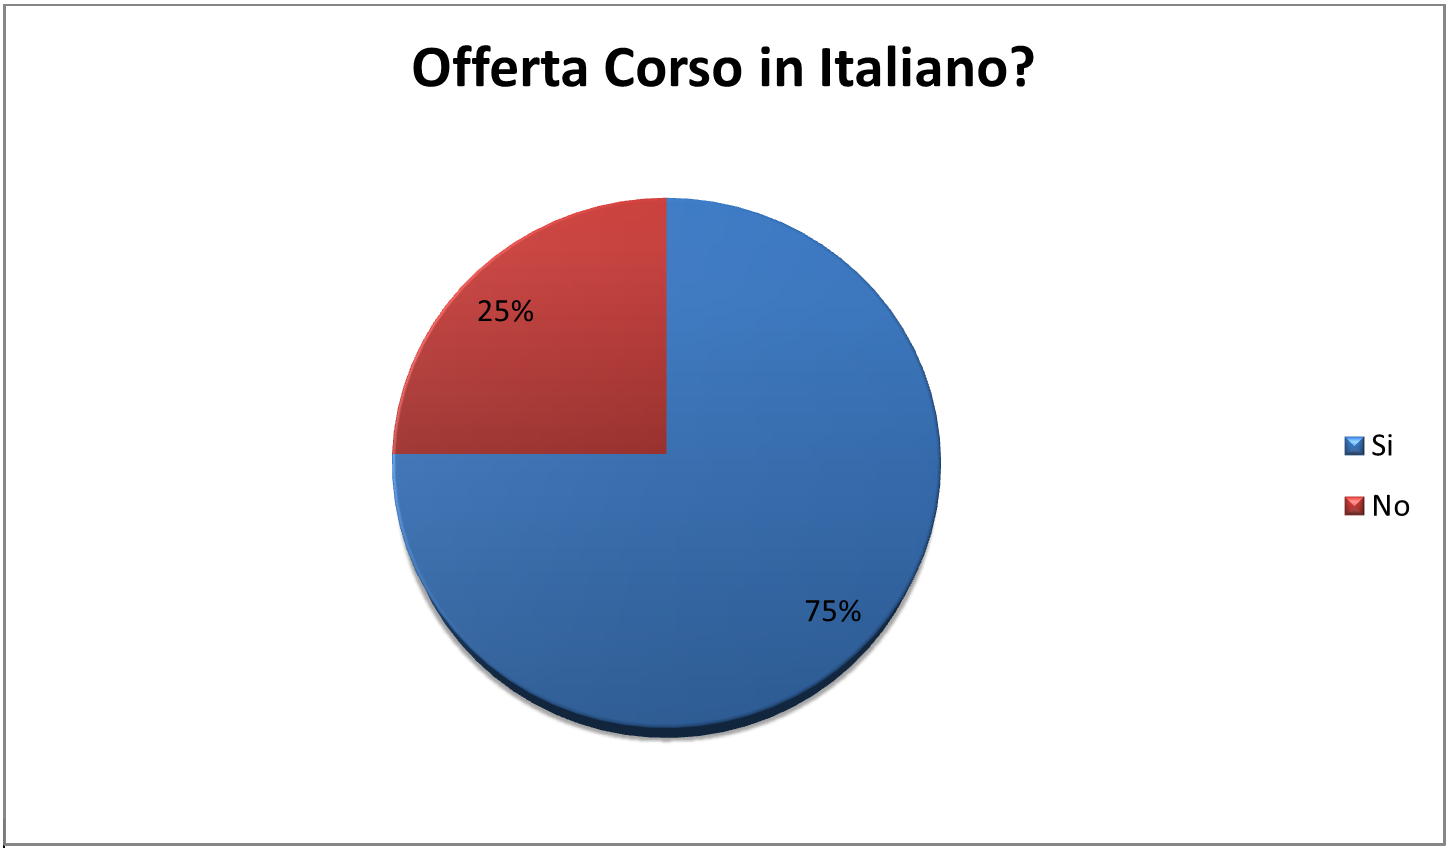
\includegraphics[scale=0.20]{images/cap4/concorrenza/corsoItaliano.png}
\caption{Offerta corso in italiano}
\end{figure}

Un altro importante fattore discriminante è il costo dei corsi.

% inserire una figura
\begin{figure}[H]
\centering
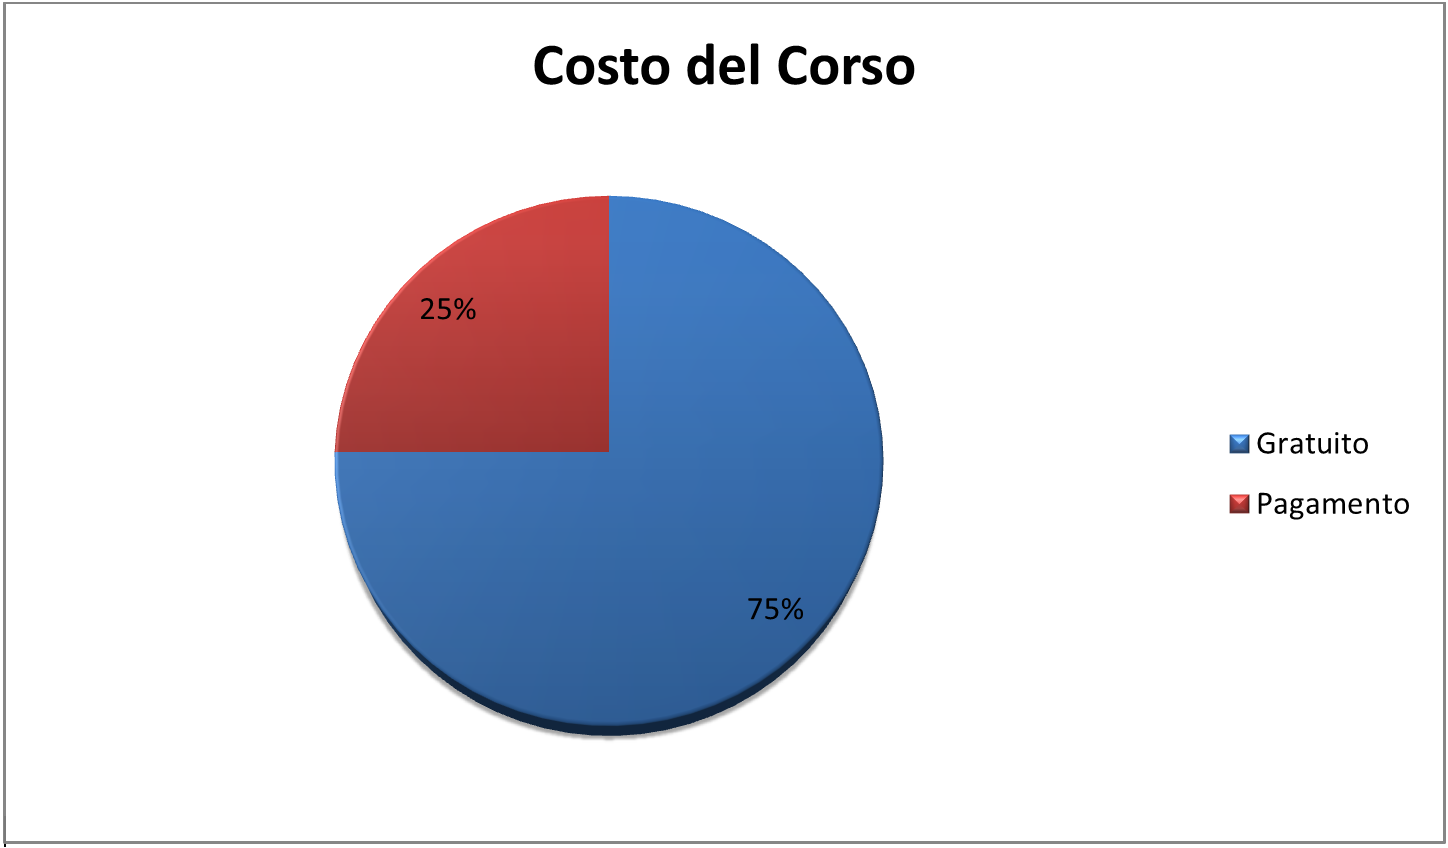
\includegraphics[scale=0.20]{images/cap4/concorrenza/costoCorso.png}
\caption{Costo del corso}
\end{figure}

Passiamo ora ad analizzare quanti offrono una certificazione riconosciuta.

% inserire una figura
\begin{figure}[H]
\centering
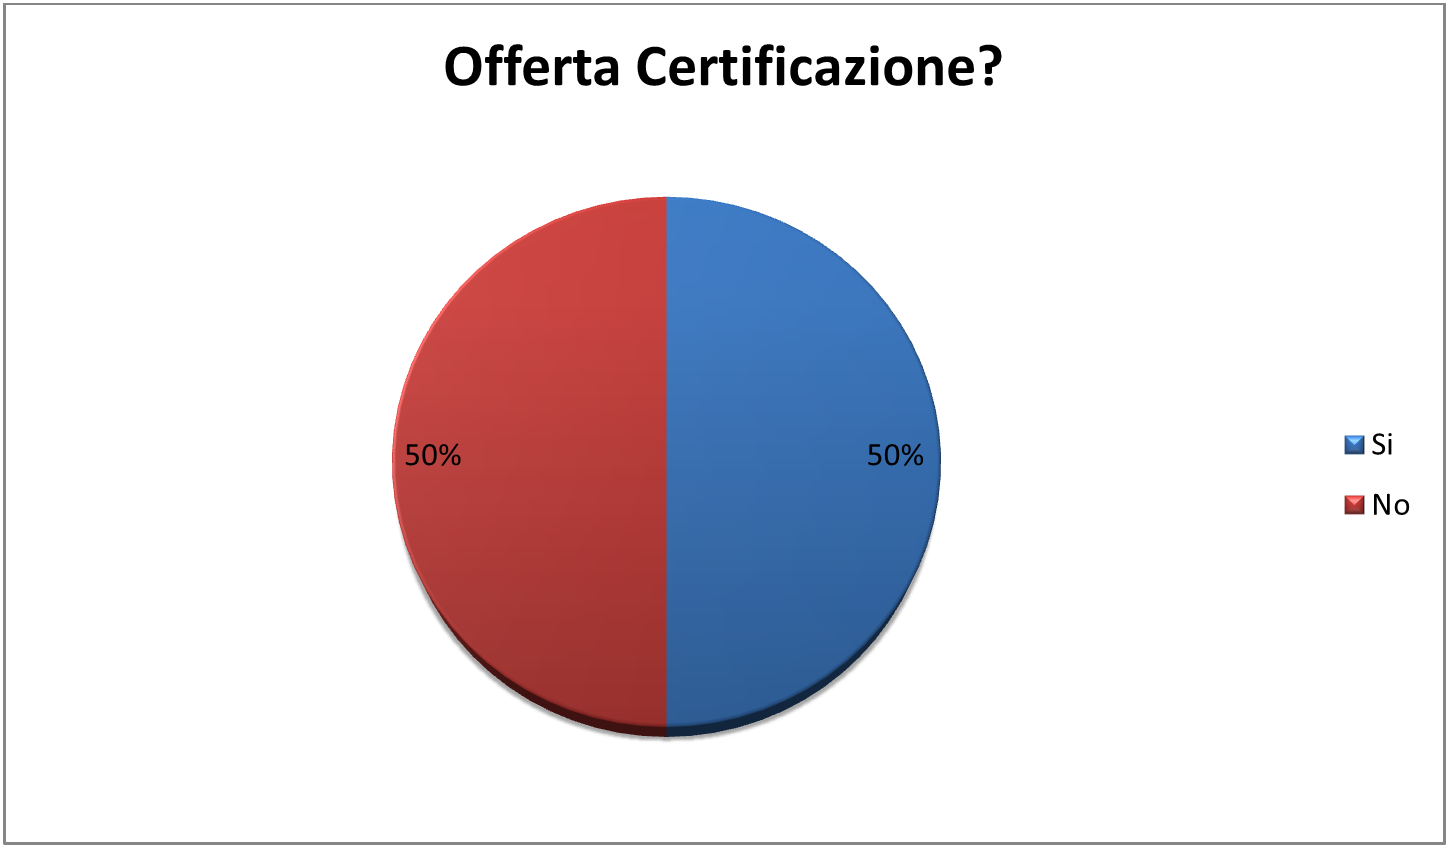
\includegraphics[scale=0.20]{images/cap4/concorrenza/offertaCertificazione.png}
\caption{Offerta certificazione}
\end{figure}

E infine analizziamo quanti di questi utilizzano principi di gamification nei propri corsi.

% inserire una figura
\begin{figure}[H]
\centering
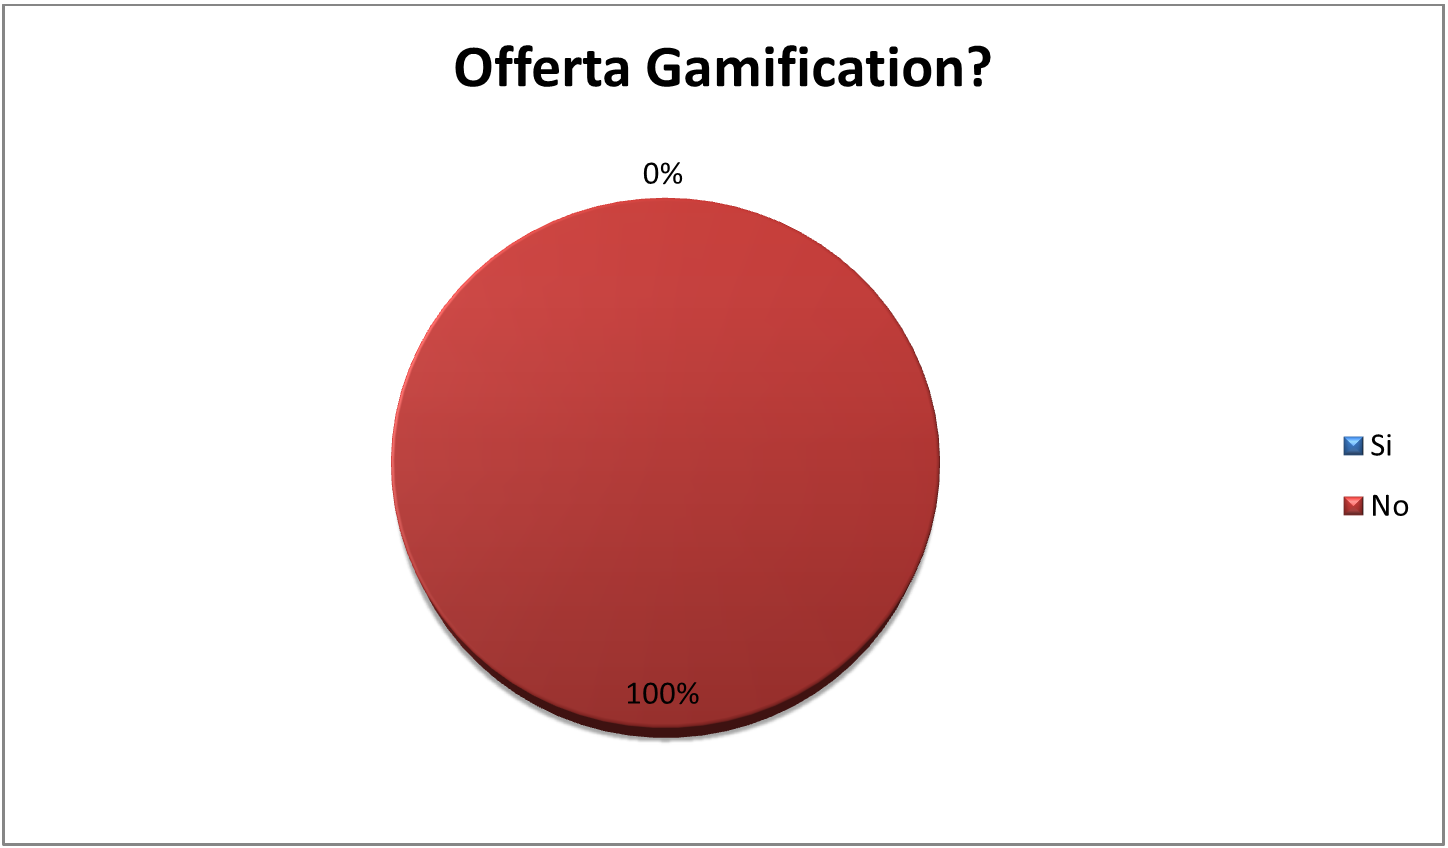
\includegraphics[scale=0.20]{images/cap4/concorrenza/principiGamification.png}
\caption{Uso di principi di Gamification}
\end{figure}

\section{Conclusioni}

Dai dati raccolti in precedenza, possiamo evincere le seguenti conclusioni:

\begin{enumerate}
	\item Nel mercato dei lavoratori in \textbf{mobilità} attualmente non abbiamo rivali. Woty permettere di coprire questa nicchia in maniera esclusiva. È tuttavia consigliato il monitoraggio delle due applicazioni \textbf{mobile} rilevate o lo sviluppo di nuove app per impedire di perdere questa egemonia.
	
	\item In ambito desktop o in quello dei corsi frontali il nostro unico competitor è \textbf{ANFOS} (poiché l'altro possibile concorrente si rifà a quest'ultimo per i test e il listino prezzi). Finché la nostra offerta sarà superiore in convenienza rispetto all'offerta di ANFOS risulterà unica poiché offre elementi di gamification, permette l'accesso al servizio anche ai lavoratori in mobilità e permette di evitare la perdita di giorni lavorativi per frequentare le lezioni frontali.
	
	\item Vista la grande diffusione di corsi gratuiti sulla sicurezza sul lavoro, è necessario che il nostro software rilasci attestati validi \textbf{certificati} a norma di decreto legislativo 81/2008 per essere commercializzato.
Per poter rilasciare questi attestati, tutti i materiali del nostro corso devono essere redatti da un esperto di sicurezza certificato (si veda il cap. \ref{AnalisiCosti} \textit{Analisi dei costi}).\\
Per ammortizzare questi o successivi costi richiesti in futuro, ci si affida alla possibilità di sfruttare fondi europei destinati a iniziative sulla sicurezza sul lavoro.

\end{enumerate}







%####################################################
%   cap "ziero"
%####################################################

\chapter{Business Model}

Il presente descrive il modello di business inteso per la commercializzazione del software Woty. Verranno delineate le caratteristiche di commercializzazione del software, le loro motivazioni e i punti di forza e debolezza.

\section{Ampliamento di Mercato}
Il nostro prodotto inizialmente sarà commercializzato solamente in Italia per approfondire ulteriormente la fattibilità/successo dello stesso e per consolidare la struttura IT su cui si basa e il ramo dell'azienda che segue il progetto.\\
In caso la nostra iniziativa abbia successo e volessimo ampliare il nostro mercato anche in altre regioni
dell'Europa, è da sottolineare che la nostra applicazione supporta già numerose lingue e senza ulteriori fasi
di sviluppo ci si potrebbe dedicare solamente all'ampliamento della struttura IT e della studio dei mercati
europei e delle legislazioni dei singoli paesi in cui si vorrebbe commercializzare il prodotto.

\section{Software as a service}
Come spiegato in precedenza sui dettagli tecnici, il cliente usufruisce dei servizi del software tramite il browser. A differenza dello standard per questo tipo di servizi, Woty necessita di un maggiore grado di rapporto con il cliente a causa della natura eterogenea delle necessità dei clienti. Ogni cliente può avere richieste diverse che almeno inizialmente sono trattate come commesse e sviluppate ad-hoc. In un momento successivo si può pensare alla standardizzazione del servizio e quindi all'apertura verso il mercato mondiale.

%\subsection{Implicazioni commerciali}

%\subsubsection{Acquisizione del cliente}
%Inizialmente vanno gestite commesse per la standardizzazione delle funzionalità. Successivamente il cliente si %arrangia, iscrivendosi e utilizzando autonomamente il servizio.


\section{Business Model}
Andiamo ora a descrivere il business model scelto per affrontare il mercato con il nostro software sia con una descrizione testuale sia con un Canvas che racchiude i concetti chiave.

\subsection{Customer segments}
I customer segment sono i segmenti di mercato al quale il nostro prodotto è rivolto. Il software è stato realizzato tenendo conto delle esigenze specifiche di quelle imprese che hanno bisogno di trovare un'alternativa efficace ai corsi frontali sulla sicurezza, quindi seguiamo un cosiddetto mercato di nicchia, con richieste particolari e raggiungibile tramite canali precisi. \\
Quindi Woty mira a farsi spazio nel mercato attirando clienti che vogliono ridurre le spese per gestire la sicurezza sul lavoro o comunque vogliono affrontare la questione con un approccio innovativo e coinvolgente per i propri dipendenti. \\
Stiamo comunque parlando di un modello B2B, cioè un Business-to-business, che quindi implica che l'acquirente diretto è una società, che poi offrirà il servizio ai suoi dipendenti.\\
\\ \textbf{Concetti chiave:}
\begin{itemize}
\item \textbf{Mercato di nicchia}
\item \textbf{Esigenze specifiche}
\item \textbf{Canali dedicati}
\end{itemize}

\subsection{Value Propositions}
Value Proposition indica il valore proposto al pubblico ed il valore per il quale un customer segment dovrebbe scegliere il nostro prodotto anziché quello di un eventuale concorrente. Questo valore è creato in Woty grazie all'unione di più fattoti chiave che nell'insieme creano un prodotto interessante per la fascia di mercato di destinazione. Vediamoli nello specifico:

\begin{itemize}
\item \textbf{Innovazione}: il software Woty offre un servizio innovativo, che si fa spazio in un settore di mercato ancora poco esplorato. Cerchiamo così di farci notare tra tutti quelli che offrono un servizio simile ma con metodi più tradizionali, perché un mercato non ancora molto sviluppato offre grandi potenzialità di crescita.
\item \textbf{Cost Reduction}: oltre ad innovazione il nostro prodotto offre un metodo per ridurre i costi di formazione del personale, un incentivo non da sottovalutare per utilizzare il nostro prodotto. Sostituendo i corsi frontali sulla sicurezza sul lavoro il nostro software allevia il cliente anche dei costi per sostenere questi corsi, garantendo un margine di risparmio sostanziale. Oltre a pesare sulle finanze del cliente permette un maggiore coinvolgimento da parte dell'utilizzatore finale del prodotto, che spesso può portare ad una formazione del personale migliore.
\item \textbf{Usabilità}: infine il nostro prodotto offre un interfaccia utente facile ed intuitiva per appunto spronare e facilitare l'utilizzo anche da parte di quei clienti meno propensi alle tecnologie informatiche. La parte "social" del nostro prodotto può far ritrovare un ambiente familiare grazie alla grande diffusione dei social network degli ultimi anni.
\end{itemize}

\subsection{Channels}

I canali sono i metodi che abbiamo a disposizione per far arrivare e recepire informazioni e messaggi dalla e verso la clientela, vediamo i channel principali e la loro suddivisione:

\subsubsection{Marketing e pubblicità}

\begin{itemize}
\item \textbf{Inserzioni}\\
Per effettuare un marketing mirato, si è scelto di apportare delle inserzioni pubblicitarie su riviste specialistiche. \\
Tra queste vi è QuotidianoSicurezza.it che consiste in una rivista periodica di aggiornamenti e news sul mondo della sicurezza sul lavoro. In questo modo si può facilmente raggiungere utenti interessati all'ambito della sicurezza sul lavoro e ai metodi innovativi per l'insegnamento della sicurezza sul lavoro in ambito aziendale.\\
QuotidianoSicurezza.it dispone anche di una apposita app per smartphone nella quale vengono visualizzate le news e le inserzioni presenti nel quotidiano.\\
Il preventivo proposto dal quotidiano per la pubblicazione di inserzioni pubblicitarie è di 500\EUR\ ad inserzione. Tale inserzione sarà visibile sia su quotidiano cartaceo che tramite applicazione smartphone.\\ Per il primo anno sono previste tre inserzioni per un costo complessivo di 1500\EUR.\\
\\
La camera di commercio offre la distribuzione gratuita di giornali specifici per ogni categoria commerciale o industriale iscritta al servizio, nei quali sono presenti inserzioni pubblicitarie. La pubblicazione di inserzioni in tali riviste richiede un costo di 350\EUR per inserzione.\\
Per il primo anno sono previste tre inserzioni in tale rivista con un costo complessivo di 1050\EUR.

\item \textbf{Social Network}\\
La promozione di Woty avverrà anche attraverso i principali social network Facebook, Twitter e Google+ con la creazione di una pagina Woty dedicata che ne permetterà una più facile conoscenza.\\
Tutte queste operazioni sono gratuite e non richiedono un esborso di denaro.\\
La pagina per ognuno dei social network dovrà essere mantenuta aggiornata periodicamente per avere maggiore visibilità e interesse nel visitatore.\\
Successivamente, considerato il grande successo del social network Facebook, sarà necessario creare delle inserzioni pubblicitarie in quest'ultimo; le inserzioni permettono di identificare il target di riferimento così da essere mirate per un determinato pubblico di utenza e un tetto massimo di spesa, il cui costo complessivo è previsto per 1200\EUR.

\item \textbf{Affiliazioni}\\
Trattando di sicurezza sul lavoro questo progetto ci offre la possibilità di sfruttare una serie di iniziative di
differenti enti per acquisire visibilità senza spesa alcuna.
Le due maggiori affiliazioni sono:

\begin{itemize}
	\item[\textbf{-}] \textbf{INAIL} (\url{http://www.ispesl.it/scripts/sel_app.asp?area=2&language=1&mod=3}) questo ente offre visibilità gratuita a tutte le iniziative riguardanti il tema di sicurezza degne di nota.

	\item[\textbf{-}] \textbf{EU-OSHA} (\url{http://osha.europa.eu/it}) questo ente offre visibilità gratuita a tutte le iniziative riguardanti il tema di sicurezza degne di nota, inoltre ci permette di fare conoscere la nostra applicazione in ambito europeo offrendoci in futuro la possibilità di introdurre il nostro prodotto in altre nazioni d'Europa.

\end{itemize}

\item \textbf{Rappresentanza}\\
Lavorando in un ambito particolare e delicato che tratta argomenti regolati dalla legge, il nostro progetto richiede una pubblicità mirata che non si riscontra nelle offerte delle agenzie pubblicitarie.\\ Per questo prevediamo la formazione e la mobilitazione di alcuni nostri agenti di commercio. Oltre ad una possibile rappresentanza diretta presso le maggiori aziende del territorio (sfruttando quindi anche il passaparola nell'ambiente aziendale), uno dei principali compiti previsti per queste figure è il contatto degli studi commercialisti del territorio.\\ Questi ultimi, infatti, consigliano la propria clientela in ambito di corsi/sicurezza, indirizzando spesso verso un ente o un servizio privato che offra attestati in materia.\\ Sono da chiarire di persona, ad opera del nostro rappresentante, se sono presenti costi aggiuntivi per far si che gli studi commercialisti pubblicizzino la nostra iniziativa.

\end{itemize}

\subsubsection{Farsi valutare}
\begin{itemize}
\item Il software essendo una web app dispone del sito apposito che ne permette l'utilizzo.\\
Attraverso questo sito vi sarà una apposita sezione per far conoscere Woty agli nuovi utenti indicandone utilizzo, le funzionalità, i piani abbonamento disponibili e molto altro.
\end{itemize}

\subsubsection{Vendità/delivery}
\begin{itemize}
\item Sia l'acquisto che le fornitura del servizio avvengono tramite l'applicazione web, che presenta un form di iscrizione e di scelta del tipo di abbonamento in stile \virgolette{fai da te}, dove il cliente ha tutti i dati per valutare la bontà del servizio e per effettuare la sottoscrizione.
\end{itemize}

\subsubsection{Supporto}
\begin{itemize}
\item Tematico e di post vendita: Il supporto che offriamo al cliente è di tipo self-service od automatico in quanto il cliente ha a disposizione le informazioni per risolvere gli eventuali problemi che riscontra ed in alcuni casi delle procedure guidate. Un esempio è al momento della creazione dell'account dove all'utente viene proposto uno \virgolette{wizard} che lo segue nei primi passi di configurazione. È	 comunque disponibile l'assistenza personale per problemi che non trovano riscontro nelle procedure di risoluzione classiche.
\end{itemize}

\subsection{Customer Relationships}
Descrive il tipo di relazione che la nostra società vuole avere con le fasce di mercato che utilizzano il software Woty. Principalmente cerchiamo di tenere un cosiddetto approccio self-service e di assistenza automatizzata, che quindi implica che l'utilizzatore in caso di bisogno possa trovare tutte le informazioni che gli servono per poter risolvere un eventuale problema. Queste informazioni si possono trovare sia nel manuale di utilizzo software sia negli opportuni "Help" e "About" forniti dall'applicazione Web.\\
Questa scelta è stata fatta per omogenizzare e diminuire il costo del supporto post vendita che data la prevista mole di utilizzatori potrebbe diventare problematica.\\
È comunque previsto il supporto diretto di personale in caso di necessità specifiche o in conseguenza all'acquisto di abbonamenti \textit{Gold}. \\ Tre motivazioni per aver un ottimo rapporto con i clienti.
\begin{itemize}
\item \textbf{Customer Acquisition}: fatta tramite web site e pubblicità.
\item \textbf{Customer Retention}: ottenuta anche con tecniche di gamification (badge e achievement).
\item \textbf{Upselling}: passaparola e reputazione in internet. Un cliente contento parla agli altri del nostro prodotto e consuma mediamente di più.
\end{itemize}
La parte "social" del nostro prodotto aiuta a creare una sorta di community tra gli utilizzatori, fattore che può facilmente portare ad un atteggiamento positivo verso il nostro software, grazie all'ambiente positivo.

\subsection{Revenue Streams}
In base al tipo di prodotto offerto dal software Woty e al suo utilizzo massiccio e sistematico che si avrà all'interno delle aziende acquirenti, si è ritenuto che la licenza abbonamento sia la soluzione più adeguata.\\
La licenza abbonamento prevederà una scadenza annuale rinnovabile, e non saranno richiesti ulteriori costi iniziali di attivazione, in quanto il software prevede una semplice installazione nei pc o smartphone degli utenti utilizzatori di ogni azienda ai quali sarà stato precedentemente assegnato loro un apposito account per effettuare il login alla piattaforma.\\
Per tanto non è necessaria assistenza tecnica specializzata per l'installazione del software.\\
La licenza abbonamento prevederà tre differenti tipologie: \textit{Bronze}, \textit{Silver} e \textit{Gold}.
Di seguito vengono descritte le caratteristiche di ognuna delle licenze sopra elencate:

\begin{itemize}
\item \textbf{\textit{Bronze}}:\\
consiste nella licenza minima.
Può usufruire di tutte le funzionalità base della piattaforma Woty, fatta eccezione dell'applicazione mobile che prevede l'utilizzo del software attraverso smarthphone, pertanto questo tipo di licenza non potrà prevedere account mobile tra gli utenti utilizzatori;


\item \textbf{\textit{Silver}}:\\
La licenza \textit{Silver} prevede tutte le funzionalità della licenza \textit{Bronze}, con l'aggiunta dell'utilizzo dell'applicazione mobile e quindi la possibilità di creare account mobile.
Inoltre è previsto l'uso delle video quest, ossia di quest corredate da un video illustrativo per l'utente;


\item \textbf{\textit{Gold}}:\\
La licenza \textit{Gold} prevede tutte le funzionalità della licenza \textit{Silver}, con l'aggiunta di quest personalizzate per specifici casi o tipi di mansioni in lavori altamente specializzati.\\
Inoltre è prevista un'apposita assistenza tecnica in aggiunta al meccanismo di ticketing già presente nella piattaforma.\\
In caso di problemi urgenti sarà quindi possibile contattare telefonicamente l'assistenza che provvederà a risolvere il problema quanto prima o a fornire istruzioni sul come intervenire.\\

\end{itemize}

Per ognuna delle licenze sopra elencate sarà possibile applicare un numero di licenze di utenti utilizzatori della piattaforma in base al numero di lavoratori presenti nell'azienda acquirente. Tale numero di licenze per utente, potrà essere modificato annualmente allo scadere della licenza annua.\\
Sono previste 5 fasce di numero di utenze che vengono elencate di seguito con i rispettivi costi in base al tipo di licenza scelta:

\begin{table}[ht]

\caption{Licenze previste Woty}
\centering
\begin{tabular}{|p{3cm}|p{1,6cm}|p{1,6cm}|p{1,6cm}|}
\hline
\rule[-2mm]{0mm}{0.7cm}
\textbf{Fascia utenti} &	"\textbf{\textit{Bronze}}" 	& 	"\textbf{\textit{Silver}}" 	& 	"\textbf{\textit{Gold}}"\\
\hline
\rule[-2mm]{0mm}{0.7cm}
"meno di 50"	    &			"500\EUR"	        & 			"750\EUR"			& 			"1.000\EUR"		\\
\hline
\rule[-2mm]{0mm}{0.7cm}
"da 50 a 200"	&			"1.250\EUR"			& 			"1.875\EUR"			& 			"2.500\EUR"		\\
\hline
\rule[-2mm]{0mm}{0.7cm}
"da 200 a 500"	&			"3.500\EUR"			& 			"5.250\EUR"			& 			"7.000\EUR"		\\
\hline
\rule[-2mm]{0mm}{0.7cm}
"da 500 a 1000"	&			"7.500\EUR"			& 			"11.250\EUR"			& 			"15.000\EUR"		\\
\hline
\rule[-2mm]{0mm}{0.7cm}
"più di 1000"	&			"10.000\EUR"			& 			"15.000\EUR"			& 			"20.000\EUR"		\\
\hline
\end{tabular}
\end{table}

\subsection{Key Resources}
Sono le risorse chiave necessarie a fornire e garantire la nostra Value Proposition. Senz'altro in Woty la risorsa che ci permette di offrire il valore che ci contraddistingue è la piattaforma in sé, dato che il suo funzionamento è il principale servizio che offriamo al cliente. Ma le risorse non sono solo fisiche, anche la capacità di offrire nuovi incentivi e soluzioni riguardanti la gamification e i funzionamenti dei "giochi" della piattaforma ideati dal nostro team possono fare la differenza tra un buon prodotto e un prodotto ottimo. Vediamo in dettaglio:
\begin{itemize}
\item \textbf{Risorse fisiche}: struttura fisica che fa funzionare tutto il servizio, deve essere gestita e manutenuta nel migliore dei modi per ridurre le spese ed eventuali incidenti.
\item \textbf{Risorse umane}: team di sviluppo con un know-how tale da organizzare un esperienza di utilizzo e approccio alla gamification che invoglia il cliente all'utilizzo.
\item \textbf{Intellettuali}: miriamo in un periodo di tempo relativamente breve di avere un database di quest e di dati riguardanti la gamification molto amplio, risorsa che può fare la differenza con i nostri competitor.
\end{itemize}

\subsection{Key Activities}
Sono le attività che garantiscono che la nostra Value Proposition possa essere generata, mantenuta e consegnata al cliente. La principale attività che la nostra società deve eseguire è la gestione delle piattaforma che sorregge tutto il software Woty, quindi bisogna controllare sia le risorse fisiche (server) che il software (possibili bug e versioni 2.x).\\
Attività importante è anche la consulenza ai clienti, sia quella personale sia quella automatica (software) che ha bisogno di continue migliorie.\\
Non dimentichiamo che comunque siamo un team di sviluppo software e che quindi un attività fondamentale è quella di aggiornare e migliorare continuamente il nostro codice, sia quello già esistente che quello futuro.

\subsection{Key Partners}
Sono i partner dei quali ci avvaliamo per ottenere vantaggi sia economici che legati all'out\-sourcing. Vediamoli in dettaglio:
\begin{itemize}
\item \textbf{Pubblicità}: la pubblicità sarà in parte affidata e gestita da partner esterni, cosa più economica e conveniente che formare del personale interno.
\item \textbf{Infrastruttura hardware}: la piattaforma hardware sarà fornita e custodita da società terze specializzate in questo tipo di business.	
\item \textbf{Altre alleanze}, sia di tipo strategico che per riduzione dei rischi non sono state programmate per adesso, principalmente per il poco sviluppo del mercato in questo ambito. Non escludiamo partnership con altre società per rafforzare il nostro business in futuro.
\end{itemize}

\subsection{Cost Structure}
È l'insieme delle spese che la nostra attività comporta, sia legate alle infrastrutture che al marketing che alla ricerca e sviluppo. Più è bassa in relazione alle entrate maggiore sarà il reddito della società, quindi si cerca di minimizzare le spese, spinti da un economia di costo più che da una da valore.
\begin{itemize}
\item \textbf{Costi fissi}: i costi fissi previsti per offrire il servizio al cliente sono principalmente quelli legati alla struttura fisica che mantiene attivo il servizio, quelli per il supporto post vendita e gli stipendi di tutti i membri del gruppo.
\item \textbf{Costi variabili}: sono quelli legati alla parte di pubblicità, alle inserzioni e quelli legati alle partnership che eseguono lavori su commissione.
\end{itemize}

Seguiamo un economia di scala in quanto più clienti riusciamo a soddisfare con la nostra infrastruttura e meno ci costerà mantenerla in proporzione ai ricavi. 

\newpage

\subsection{Canvas}

Di seguito viene rappresentato graficamente il riassunto del business model descritto tramite il Canvas dei modelli dei business.

\begin{figure}[H]
\centering
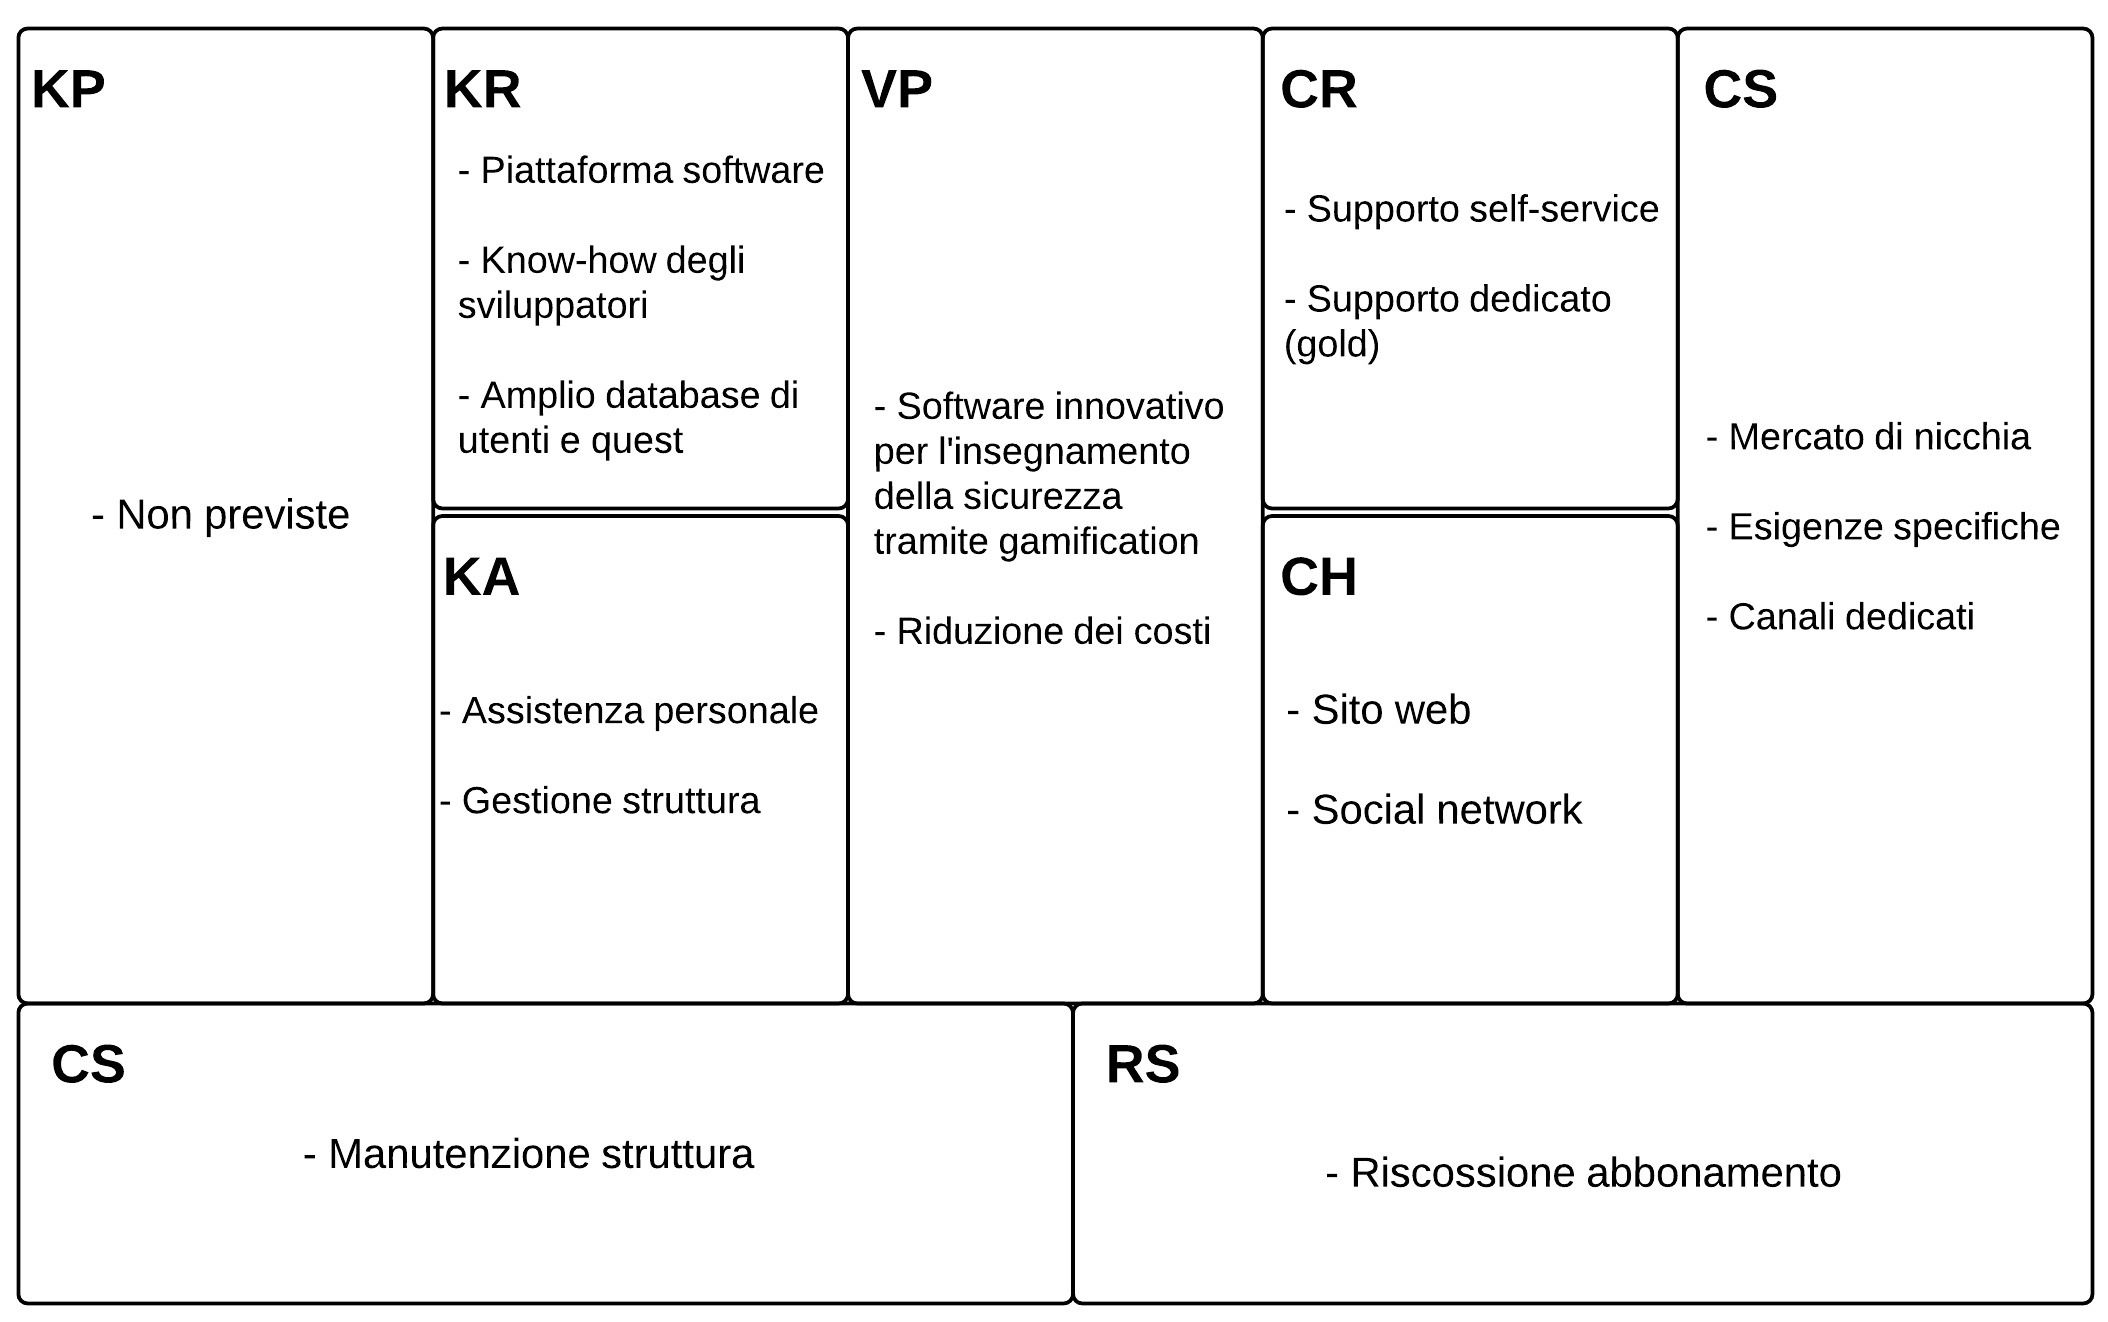
\includegraphics[scale=0.8]{images/cap5/BM.png}
\caption{Business Model Canvas}
\end{figure}


\section{Modifiche al software}
A seguito dell'analisi di mercato, dell'analisi sulla concorrenza e dello studio sul business model, si sono riscontrate delle modifiche da effettuare al software in modo da poter essere più competitivo nel mercato e trovare una più facile diffusione presso le aziende.\\
Verrà pertanto riportato in seguito un elenco descrittivo di tali modifiche con l'aggiunta anche delle evenutali estensibilità del sistema, in previsione di modifiche future o adattamenti in fase di manutenzione del software dovuti o a cambiamenti dei requisiti o al riscontro di malfunzionamenti.

\begin{itemize}
\item il sistema già progettato per il supporto al multi lingua, ora dispone solamente delle lingue italiano ed inglese. In seguido allo studio nell'analisi di mercato, si è osservato che i lavoratori stranieri presenti in Italia sono una percentuale non ininfluente. Andranno pertanto aggiunte le traduzioni adeguate per le prinicipali nazionalità dei lavoratori stranienieri;
\underline{tempistiche}: un mese per programmatore e un esperto di lingue;\\
\underline{costo stimato}: 2000\EUR.


\item essendo l'applicazione mobile uno dei punti di forza della piattaforma Woty rispetto ai concorrenti, si prevede la realizzazione dell'applicazione mobile anche per le piattaforme Windows Phone e iOS.
Si potrà così ampliare la gamma dei dispositivi supportati aumentando l'usabilità della piattaforma;\\
\underline{tempistiche}: un mese per due programmatori;\\
\underline{costo stimato}: 4000\EUR.


\item dagli studi sulla concorrenza è emerso come l'uso della gamification per l'insegnamento della sicurezza sul lavoro sia un'innovazione; si prevede quindi di ampliare tale fattore permettendo al sistema la creazione e visualizzazione di nuovi badge;\\
\underline{tempistiche}: una settimana e mezza per un programmatore\\
\underline{costo stimato}: 900\EUR.


\item altro fattore per l'aumento della gamification consiste nell’inserimento di un tempo limite per la risoluzione della quest, l'utente sarà così più motivato nel rispondere correttamente secondo le proprie conoscenze acquisite;\\
\underline{tempistiche}: una settimana per due programmatori\\
\underline{costo stimato}: 600\EUR.

\end{itemize}


Complessivamente gli interventi hanno un costo di circa 7.500 \EUR.





%--------------------------- CONCORRENZA
%####################################################
%   cap Stefano
%##################################################

\chapter{Analisi dei costi}
\label{AnalisiCosti}

In questo capitolo vengono discussi i costi e i guadagni previsti dall'adozione del modello di business descritto precedentemente. Saranno inoltre riportati e discussi i tempi e i costi dedicati allo sviluppo di questo progetto.

\section{Prospetto riassuntivo business model}

\subsection{Consuntivo per la prima realizzazione del Software Woty}

\red{LORY DIO£!\#?, PER ME STA ROBA NON CENTRA UN CA**O!}\\
Di seguito viene proposto il consuntivo economico ed il riassunto della suddivisione dei ruoli effettuata dal gruppo durante il primo  sviluppo del prodotto software denominato \texttt{Woty}.\\

I costi della fase di sviluppo del software sono stati calcolati in funzione dei costi orari riportati nella seguente tabella:

\begin{longtable}{|p{4cm} p{1cm}|p{3cm}|}
\caption{Costi/Ora per ruolo}\\
\hline
\endfirsthead
\multicolumn{3}{r}{\textit{(Continua alla pagina successiva)}}
\endfoot
\multicolumn{3}{l}{\textit{(Continua dalla pagina precedente)}}
\endhead

\endlastfoot
\textbf{Ruolo}& \textbf{}& \textbf{Costo/Ora in \EUR}\\
\hline
Responsabile	& (RE) & 30\\
\hline
Amministratore	& (AM) & 20\\
\hline
Analista	    & (AN) & 25\\
\hline
Progettista	    & (PT) & 22\\
\hline
Programmatore	& (PM) & 15\\
\hline
Verificatore	& (VR) & 15\\
\hline
\end{longtable}

Di seguito si riportano i costi sostenuti per ogni ruoli impiegato nello sviluppo del progetto in forma tabellare.

\begin{table}[H]
\caption{Consuntivo costi totale}
\label{costiTotaliConsuntivo}
\centering
\begin{tabular}{|p{3cm} | p{1cm}|p{1cm}| p{1cm}| p{1cm}| p{1cm}| p{1cm}| p{1cm}|}
\hline
\textbf{Ruolo}           & RE   &   AM  &   AN  &  PT  &  PM  &  VR  &  Totale      \\
\hline
\textbf{Consuntivo} 		& 900  &  1060 &  1750 & 3652 & 2295 & 3945 & \textbf{13602} \\
\hline
\end{tabular}
\end{table}

In figura \ref{costiTotPerRuoloCons} viene proposta la ripartizione dei costi totali per ruolo utilizzato nel progetto.

% inserire una figura
\begin{figure}[h]
\centering
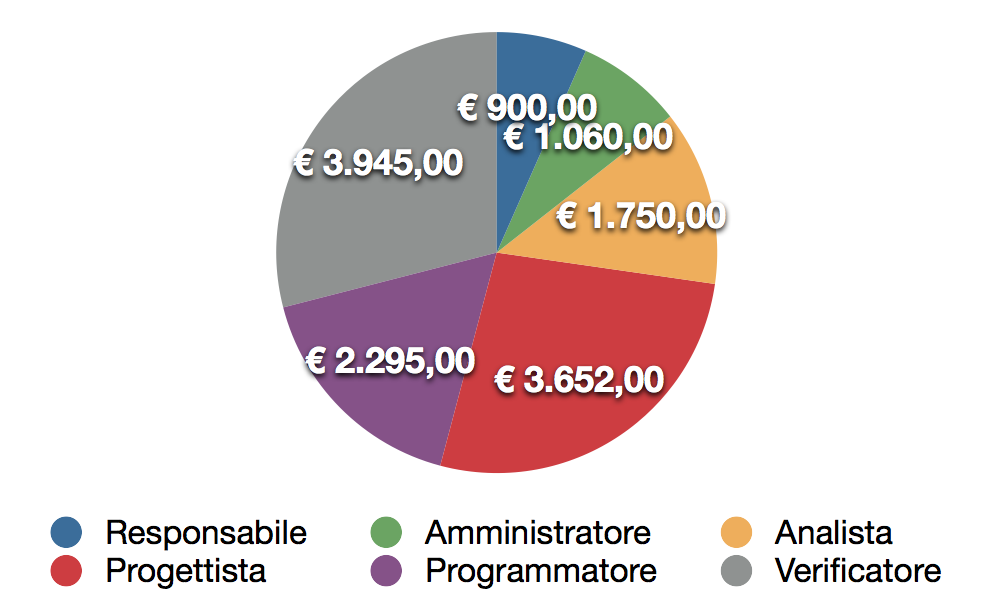
\includegraphics[scale=0.25]{images/cap6/costiPerRuoloConsuntivo.png} % vedi Lateximpazienye pg67
\caption{Costi totali per ruolo}
\label{costiTotPerRuoloCons}
\end{figure}


\newpage

\subsection{Analisi dei costi del business model}

Di seguito si riportano costi e guadagni previsti dal business model.

\subsubsection{Costi iniziali}
\begin{itemize}
	\item \textbf{Primo sviluppo del software:} 13602 \EUR.
	\item \textbf{Nuove funzionalità tecniche:} \red{(se ci sono)}
	\item \textbf{Consulenza legale:} \red{(se ci servirà)}
	\item \textbf{Campagna di marketing:} \red{(...)}
\end{itemize}


\subsubsection{Costi fissi}

\begin{itemize}
	\item \textbf{Manutenzione acquisto o la locazione del server:} \red{Preeeettoooo}
\end{itemize}

\subsubsection{Costi variabili}

\red{//TODO?}

\subsubsection{Utenti e guadagni previsti}

\red{//TODO}

\subsubsection{Analisi di Breakeven}

\red{NON SO SE LA FARÒ}

\section{Consuntivo finale del progetto}

Di seguito è riportato il riassunto del quantitativo orario che ogni risorsa ha dedicato al progetto, l'indicazione del costo medio orario (CMO) ed un prospetto indicante i costi totali sostenuti per il progetto.
Questi dati sono stati calcolati nella fase finale del progetto e rappresentano il costo finale del lavoro svolto dalle varie figure professionali impegnate nel progetto.\\
Il consuntivo deve essere confrontato con il preventivo realizzato nelle fasi preliminari per avere un migliore riscontro delle variazioni rispetto alla previsione iniziale.\\
Viene ora riproposto il CMO delle varie figure professionali impegnate nel progetto:	

\begin{longtable}{ | p{5cm} | p{3.4cm} |}
\caption{Compenso orario delle figure professionali}\\
\hline
\endfirsthead
\multicolumn{2}{r}{\textit{(Continua alla pagina successiva)}}
\endfoot
\multicolumn{2}{l}{\textit{(Continua dalla pagina precedente)}}
\endhead
\hline
\endlastfoot
\textbf{Figura professionale} \ & \textbf{CMO}\\
\hline
\rule[-2mm]{0mm}{0.7cm}
Capo progetto & \EUR \ 40 \\
\hline
\rule[-2mm]{0mm}{0.7cm}
Esperto mercato & \EUR \ 25 \\
\hline
\rule[-2mm]{0mm}{0.7cm}
Esperto marketing & \EUR \ 25 \\
\hline
\rule[-2mm]{0mm}{0.7cm}
Tecnico informatico & \EUR \ 30 \\
\hline
\end{longtable}

Dopo aver osservato il compenso orario per ogni figura impegnata nel progetto viene visualizzato il costo totale dato dal lavoro di ognuna di esse.\\ Tra parentesi possiamo notare le variazioni effettuate dal preventivo stimato nel cap.\ref{pianificazioneDelLavoro} \textit{Pianificazione del lavoro}.

\begin{longtable}{ | p{6cm} | p{3.5cm} | p{4cm} |}
\caption{Consuntivo costi per ogni figura professionale}\\
\hline
\endfirsthead
\multicolumn{3}{r}{\textit{(Continua alla pagina successiva)}}
\endfoot
\multicolumn{3}{l}{\textit{(Continua dalla pagina precedente)}}
\endhead
\hline
\endlastfoot
\textbf{Figura professionale} \ & \textbf{Ore consuntivate} \ & \textbf{Costi consuntivati} \\
\hline
\rule[-2mm]{0mm}{0.7cm}
Capo progetto & 95 (\textbf{-5}) & \EUR \ 3.800 (\textbf{-200})\\
\hline
\rule[-2mm]{0mm}{0.7cm}
Esperto mercato & 124 (\textbf{-4})& \EUR \ 3.100 (\textbf{-100})\\
\hline
\rule[-2mm]{0mm}{0.7cm}
Esperto marketing & 95 (\textbf{+5}) & \EUR \ 2.375 (\textbf{+125})\\
\hline
\rule[-2mm]{0mm}{0.7cm}
Tecnico informatico & 102 (\textbf{+2}) & \EUR \ 3.060 (\textbf{+60})\\
\hline
\rule[-2mm]{0mm}{0.7cm}
\textbf{Totale} & \textbf{406} (\textbf{-2}) & \textbf{\EUR \ 12.335} (\textbf{-115})\\
\hline
\end{longtable}

Si analizzano ora le variazioni alle ore e ai costi preventivati. In generale le ore impiegate hanno rispecchiato la pianificazione iniziale abbastanza fedelmente. Le variazioni sono state minime per ogni ruolo in particolare:

\begin{itemize}
	\item Il \textbf{capo progetto} e l'\textbf{esperto di mercato} hanno sostenuto un numero di ore leggermente inferiore a quelle previste in fase di pianificazione. Questo dovuto probabilmente ad una sovrastima iniziale per quanto riguarda il controllo del progetto e l'analisi della situazione della sicurezza nel lavoro nel mercato attuale.
	\item L'\textbf{esperto in marketing} e il \textbf{tecnico informatico} hanno svolto un numero di ore leggermente maggiore rispetto al preventivo. Le ore in eccesso sono state svolte per contrastare una leggera sottostima nella pianificazione.\\ Sottostima rilevata soprattutto per quanto riguarda l'analisi dei concorrenti nell'ambito della sicurezza e gamification svolta nel marketing, e la descrizione tecnica del prodotto per quanto riguarda il lavoro del nostro tecnico informatico.
\end{itemize}

Date queste variazioni sono state svolte 2 ore in meno rispetto a quelle totali preventivate, fatto che ha portato ad una appena percettibile diminuzione dei costi totali.\\

Si riassumono infine le variazioni nei costi dal punto di vista delle varie fasi svolte nello sviluppo del progetto nella tabella seguente.\\ Tra parentesi possiamo notare le variazioni effettuate dal preventivo stimato nel cap.\ref{pianificazioneDelLavoro} \textit{Pianificazione del lavoro}.


\begin{longtable}{ | p{6cm} | p{4.4cm} |}
\caption{Consuntivo costi per fase di progetto}\\
\hline
\endfirsthead
\multicolumn{2}{r}{\textit{(Continua alla pagina successiva)}}
\endfoot
\multicolumn{2}{l}{\textit{(Continua dalla pagina precedente)}}
\endhead
\hline
\endlastfoot
\textbf{Fase di progetto} \ & \textbf{Costi consuntivati}\\
\hline
\rule[-2mm]{0mm}{0.7cm}
Pianificazione e Analisi prodotto & \EUR \ 1.150 \\
\hline
\rule[-2mm]{0mm}{0.7cm}
Analisi di mercato & \EUR \ 1.675 (\textbf{+75})\\
\hline
\rule[-2mm]{0mm}{0.7cm}
Studio di fattibilità & \EUR \ 2.050 (\textbf{+110})\\
\hline
\rule[-2mm]{0mm}{0.7cm}
Verifica progressi & \EUR \ 485\\
\hline
\rule[-2mm]{0mm}{0.7cm}
Progettazione business model & \EUR \ 4.655 (\textbf{-195})\\
\hline
\rule[-2mm]{0mm}{0.7cm}
Stime conclusive & \EUR \ 2.320 (\textbf{-105})\\
\hline
\rule[-2mm]{0mm}{0.7cm}
\textbf{Totale} & \textbf{\EUR \ 12.335} (\textbf{-115})\\
\hline
\end{longtable}

Come si può notare le variazioni prima descritte hanno avuto ripercussioni minime nei costi del progetto nelle varie fasi. Vi è stato un leggero aumento dei costi nella fase in cui si è andato ad analizzare il mondo della sicurezza nel lavoro, che dato l'argomento è risultato molto vasto.\\
Le diminuzioni dei costi negli altri ambiti del progetto sono da imputare principalmente alla sovrastima iniziale nelle ore previste per il capo progetto, che essendo la figura professionale con CMO più elevato comporta conseguenze maggiori nei costi rispetto agli altri ruoli.



\end{document}
